% Options for packages loaded elsewhere
\PassOptionsToPackage{unicode}{hyperref}
\PassOptionsToPackage{hyphens}{url}
%
\documentclass[
]{book}
\usepackage{amsmath,amssymb}
\usepackage{iftex}
\ifPDFTeX
  \usepackage[T1]{fontenc}
  \usepackage[utf8]{inputenc}
  \usepackage{textcomp} % provide euro and other symbols
\else % if luatex or xetex
  \usepackage{unicode-math} % this also loads fontspec
  \defaultfontfeatures{Scale=MatchLowercase}
  \defaultfontfeatures[\rmfamily]{Ligatures=TeX,Scale=1}
\fi
\usepackage{lmodern}
\ifPDFTeX\else
  % xetex/luatex font selection
\fi
% Use upquote if available, for straight quotes in verbatim environments
\IfFileExists{upquote.sty}{\usepackage{upquote}}{}
\IfFileExists{microtype.sty}{% use microtype if available
  \usepackage[]{microtype}
  \UseMicrotypeSet[protrusion]{basicmath} % disable protrusion for tt fonts
}{}
\makeatletter
\@ifundefined{KOMAClassName}{% if non-KOMA class
  \IfFileExists{parskip.sty}{%
    \usepackage{parskip}
  }{% else
    \setlength{\parindent}{0pt}
    \setlength{\parskip}{6pt plus 2pt minus 1pt}}
}{% if KOMA class
  \KOMAoptions{parskip=half}}
\makeatother
\usepackage{xcolor}
\usepackage{color}
\usepackage{fancyvrb}
\newcommand{\VerbBar}{|}
\newcommand{\VERB}{\Verb[commandchars=\\\{\}]}
\DefineVerbatimEnvironment{Highlighting}{Verbatim}{commandchars=\\\{\}}
% Add ',fontsize=\small' for more characters per line
\usepackage{framed}
\definecolor{shadecolor}{RGB}{248,248,248}
\newenvironment{Shaded}{\begin{snugshade}}{\end{snugshade}}
\newcommand{\AlertTok}[1]{\textcolor[rgb]{0.94,0.16,0.16}{#1}}
\newcommand{\AnnotationTok}[1]{\textcolor[rgb]{0.56,0.35,0.01}{\textbf{\textit{#1}}}}
\newcommand{\AttributeTok}[1]{\textcolor[rgb]{0.13,0.29,0.53}{#1}}
\newcommand{\BaseNTok}[1]{\textcolor[rgb]{0.00,0.00,0.81}{#1}}
\newcommand{\BuiltInTok}[1]{#1}
\newcommand{\CharTok}[1]{\textcolor[rgb]{0.31,0.60,0.02}{#1}}
\newcommand{\CommentTok}[1]{\textcolor[rgb]{0.56,0.35,0.01}{\textit{#1}}}
\newcommand{\CommentVarTok}[1]{\textcolor[rgb]{0.56,0.35,0.01}{\textbf{\textit{#1}}}}
\newcommand{\ConstantTok}[1]{\textcolor[rgb]{0.56,0.35,0.01}{#1}}
\newcommand{\ControlFlowTok}[1]{\textcolor[rgb]{0.13,0.29,0.53}{\textbf{#1}}}
\newcommand{\DataTypeTok}[1]{\textcolor[rgb]{0.13,0.29,0.53}{#1}}
\newcommand{\DecValTok}[1]{\textcolor[rgb]{0.00,0.00,0.81}{#1}}
\newcommand{\DocumentationTok}[1]{\textcolor[rgb]{0.56,0.35,0.01}{\textbf{\textit{#1}}}}
\newcommand{\ErrorTok}[1]{\textcolor[rgb]{0.64,0.00,0.00}{\textbf{#1}}}
\newcommand{\ExtensionTok}[1]{#1}
\newcommand{\FloatTok}[1]{\textcolor[rgb]{0.00,0.00,0.81}{#1}}
\newcommand{\FunctionTok}[1]{\textcolor[rgb]{0.13,0.29,0.53}{\textbf{#1}}}
\newcommand{\ImportTok}[1]{#1}
\newcommand{\InformationTok}[1]{\textcolor[rgb]{0.56,0.35,0.01}{\textbf{\textit{#1}}}}
\newcommand{\KeywordTok}[1]{\textcolor[rgb]{0.13,0.29,0.53}{\textbf{#1}}}
\newcommand{\NormalTok}[1]{#1}
\newcommand{\OperatorTok}[1]{\textcolor[rgb]{0.81,0.36,0.00}{\textbf{#1}}}
\newcommand{\OtherTok}[1]{\textcolor[rgb]{0.56,0.35,0.01}{#1}}
\newcommand{\PreprocessorTok}[1]{\textcolor[rgb]{0.56,0.35,0.01}{\textit{#1}}}
\newcommand{\RegionMarkerTok}[1]{#1}
\newcommand{\SpecialCharTok}[1]{\textcolor[rgb]{0.81,0.36,0.00}{\textbf{#1}}}
\newcommand{\SpecialStringTok}[1]{\textcolor[rgb]{0.31,0.60,0.02}{#1}}
\newcommand{\StringTok}[1]{\textcolor[rgb]{0.31,0.60,0.02}{#1}}
\newcommand{\VariableTok}[1]{\textcolor[rgb]{0.00,0.00,0.00}{#1}}
\newcommand{\VerbatimStringTok}[1]{\textcolor[rgb]{0.31,0.60,0.02}{#1}}
\newcommand{\WarningTok}[1]{\textcolor[rgb]{0.56,0.35,0.01}{\textbf{\textit{#1}}}}
\usepackage{longtable,booktabs,array}
\usepackage{calc} % for calculating minipage widths
% Correct order of tables after \paragraph or \subparagraph
\usepackage{etoolbox}
\makeatletter
\patchcmd\longtable{\par}{\if@noskipsec\mbox{}\fi\par}{}{}
\makeatother
% Allow footnotes in longtable head/foot
\IfFileExists{footnotehyper.sty}{\usepackage{footnotehyper}}{\usepackage{footnote}}
\makesavenoteenv{longtable}
\usepackage{graphicx}
\makeatletter
\def\maxwidth{\ifdim\Gin@nat@width>\linewidth\linewidth\else\Gin@nat@width\fi}
\def\maxheight{\ifdim\Gin@nat@height>\textheight\textheight\else\Gin@nat@height\fi}
\makeatother
% Scale images if necessary, so that they will not overflow the page
% margins by default, and it is still possible to overwrite the defaults
% using explicit options in \includegraphics[width, height, ...]{}
\setkeys{Gin}{width=\maxwidth,height=\maxheight,keepaspectratio}
% Set default figure placement to htbp
\makeatletter
\def\fps@figure{htbp}
\makeatother
\setlength{\emergencystretch}{3em} % prevent overfull lines
\providecommand{\tightlist}{%
  \setlength{\itemsep}{0pt}\setlength{\parskip}{0pt}}
\setcounter{secnumdepth}{5}
\usepackage{booktabs}
\ifLuaTeX
  \usepackage{selnolig}  % disable illegal ligatures
\fi
\usepackage[style=apa,]{biblatex}
\addbibresource{book.bib}
\addbibresource{packages.bib}
\IfFileExists{bookmark.sty}{\usepackage{bookmark}}{\usepackage{hyperref}}
\IfFileExists{xurl.sty}{\usepackage{xurl}}{} % add URL line breaks if available
\urlstyle{same}
\hypersetup{
  pdftitle={Poverty and Inequality with Complex Survey Data},
  pdfauthor={Guilherme Jacob, Anthony Damico, and Djalma Pessoa},
  hidelinks,
  pdfcreator={LaTeX via pandoc}}

\title{Poverty and Inequality with Complex Survey Data}
\author{Guilherme Jacob, Anthony Damico, and Djalma Pessoa}
\date{2023-09-02}

\begin{document}
\maketitle

{
\setcounter{tocdepth}{1}
\tableofcontents
}
\hypertarget{introduction}{%
\chapter{Introduction}\label{introduction}}

The R \texttt{convey} library estimates measures of poverty, inequality, and wellbeing. There are two other R libraries covering this subject, \href{https://CRAN.R-project.org/package=vardpoor}{vardpoor} \autocite{R-vardpoor} and \href{https://CRAN.R-project.org/package=laeken}{laeken} \autocite{R-laeken}, however, only \texttt{convey} integrates seamlessly with the \href{https://CRAN.R-project.org/package=survey}{R survey package} \autocite{R-survey-article,R-survey-book,R-survey}.

\texttt{convey} is free and open-source software that runs inside the \href{https://www.r-project.org/}{R environment for statistical computing}. Anyone can review and propose changes to \href{https://github.com/ajdamico/convey}{the source code} for this software. Readers are welcome to \href{https://github.com/guilhermejacob/context/}{propose changes to this book} as well.

Individuals getting started in the field of poverty and inequality statistics might find the number of techniques described in this textbook overwhelming, especially on the topic of choosing which method might be most appropriate for each particular research question. For this reason, the authors of this textbook consider Dr.~Ija Trapeznikova's article \href{https://wol.iza.org/articles/measuring-income-inequality/long}{Measuring income inequality} an important summary of how to approach selecting between available techniques.

\hypertarget{install}{%
\section{Installation}\label{install}}

In order to work with the \texttt{convey} library, you will need to have R running on your machine. If you have never used R before, you will need to \href{https://www.r-project.org/}{install that software} before \texttt{convey} can be accessed. Once you have R loaded on your machine, you can install..

\begin{itemize}
\tightlist
\item
  the latest released version from \href{https://CRAN.R-project.org/package=convey}{CRAN} with
\end{itemize}

\begin{Shaded}
\begin{Highlighting}[]
\FunctionTok{install.packages}\NormalTok{(}\StringTok{"convey"}\NormalTok{)}
\end{Highlighting}
\end{Shaded}

\begin{itemize}
\tightlist
\item
  the latest development version from github with
\end{itemize}

\begin{Shaded}
\begin{Highlighting}[]
\NormalTok{remotes}\SpecialCharTok{::}\FunctionTok{install\_github}\NormalTok{(}\StringTok{"ajdamico/convey"}\NormalTok{)}
\end{Highlighting}
\end{Shaded}

In order to know how to cite this package, run \texttt{citation("convey")}.

\hypertarget{survey}{%
\section{Complex surveys and statistical inference}\label{survey}}

In this book, we demonstrate how to measure poverty and income concentration in a population based on microdata collected from a complex survey sample. Most surveys administered by government agencies or larger research organizations utilize a sampling design that violates the assumption of simple random sampling (SRS), including:

\begin{enumerate}
\def\labelenumi{\arabic{enumi}.}
\tightlist
\item
  Different units selection probabilities;
\item
  Clustering of units;
\item
  Stratification of clusters;
\item
  Reweighting to compensate for missing values and other adjustments.
\end{enumerate}

Therefore, basic unweighted R commands such as \texttt{mean()} or \texttt{glm()} will not properly account for the weighting nor the measures of uncertainty (such as the confidence intervals) present in the dataset. For some examples of publicly-available complex survey data sets, see \href{}{http://asdfree.com}.

Unlike other software, the R \texttt{convey} package does not require that the user specify these parameters throughout the analysis. So long as the \href{http://r-survey.r-forge.r-project.org/survey/html/svydesign.html}{svydesign object} or \href{http://r-survey.r-forge.r-project.org/survey/html/svrepdesign.html}{svrepdesign object} has been constructed properly at the outset of the analysis, the \texttt{convey} package will incorporate the survey design automatically and produce statistics and variances that take the complex sample into account.

Survey analysts familiar with the R \texttt{dplyr} syntax implemented by the \texttt{survey} library's wrapper \texttt{srvyr} package might be interested in implementing specific \texttt{convey} functions by following the \href{http://gdfe.co/srvyr/articles/extending-srvyr.html}{\texttt{svygini()} example} published by \texttt{srvyr} author Greg Freedman Ellis. Note that the full design stored by \texttt{convey\_prep()} may in some cases complicate this extension.

\hypertarget{usage-examples}{%
\section{Usage Examples}\label{usage-examples}}

In the following example, we've loaded the data set \texttt{eusilc} from the R library \href{https://CRAN.R-project.org/package=laeken}{laeken} \autocite{R-laeken}.

\begin{Shaded}
\begin{Highlighting}[]
\FunctionTok{library}\NormalTok{(laeken)}
\FunctionTok{data}\NormalTok{(eusilc)}
\end{Highlighting}
\end{Shaded}

Next, we create an object of class \texttt{survey.design} using the function \texttt{svydesign} of the \texttt{survey} library:

\begin{Shaded}
\begin{Highlighting}[]
\FunctionTok{library}\NormalTok{(survey)}
\NormalTok{des\_eusilc }\OtherTok{\textless{}{-}}
  \FunctionTok{svydesign}\NormalTok{(}
    \AttributeTok{ids =} \SpecialCharTok{\textasciitilde{}}\NormalTok{ rb030,}
    \AttributeTok{strata =}  \SpecialCharTok{\textasciitilde{}}\NormalTok{ db040,}
    \AttributeTok{weights =} \SpecialCharTok{\textasciitilde{}}\NormalTok{ rb050,}
    \AttributeTok{data =}\NormalTok{ eusilc}
\NormalTok{  )}
\end{Highlighting}
\end{Shaded}

Right after the creation of the design object \texttt{des\_eusilc}, we should use the function \texttt{convey\_prep} that adds an attribute to the survey design which saves information on the design object based upon the whole sample, needed to work with subset designs.

\begin{Shaded}
\begin{Highlighting}[]
\FunctionTok{library}\NormalTok{(convey)}
\NormalTok{des\_eusilc }\OtherTok{\textless{}{-}} \FunctionTok{convey\_prep}\NormalTok{(des\_eusilc)}
\end{Highlighting}
\end{Shaded}

To estimate the at-risk-of-poverty rate, we use the function \texttt{svyarpt}:

\begin{Shaded}
\begin{Highlighting}[]
\FunctionTok{svyarpr}\NormalTok{( }\SpecialCharTok{\textasciitilde{}}\NormalTok{ eqIncome, }\AttributeTok{design =}\NormalTok{ des\_eusilc)}
\end{Highlighting}
\end{Shaded}

\begin{verbatim}
            arpr     SE
eqIncome 0.14444 0.0028
\end{verbatim}

To estimate the at-risk-of-poverty rate across domains defined by the variable \texttt{db040} we use:

\begin{Shaded}
\begin{Highlighting}[]
\FunctionTok{svyby}\NormalTok{(}
  \SpecialCharTok{\textasciitilde{}}\NormalTok{ eqIncome,}
  \AttributeTok{by =} \SpecialCharTok{\textasciitilde{}}\NormalTok{ db040,}
  \AttributeTok{design =}\NormalTok{ des\_eusilc,}
  \AttributeTok{FUN =}\NormalTok{ svyarpr,}
  \AttributeTok{deff =} \ConstantTok{FALSE}
\NormalTok{)}
\end{Highlighting}
\end{Shaded}

\begin{verbatim}
                      db040  eqIncome          se
Burgenland       Burgenland 0.1953984 0.017202852
Carinthia         Carinthia 0.1308627 0.010606502
Lower Austria Lower Austria 0.1384362 0.006513217
Salzburg           Salzburg 0.1378734 0.011581408
Styria               Styria 0.1437464 0.007453192
Tyrol                 Tyrol 0.1530819 0.009884094
Upper Austria Upper Austria 0.1088977 0.005933094
Vienna               Vienna 0.1723468 0.007684540
Vorarlberg       Vorarlberg 0.1653731 0.013756389
\end{verbatim}

Using the same data set, we estimate the quintile share ratio:

\begin{Shaded}
\begin{Highlighting}[]
\CommentTok{\# for the whole population}
\FunctionTok{svyqsr}\NormalTok{( }\SpecialCharTok{\textasciitilde{}}\NormalTok{ eqIncome, }\AttributeTok{design =}\NormalTok{ des\_eusilc, }\AttributeTok{alpha1 =}\NormalTok{ .}\DecValTok{20}\NormalTok{)}
\end{Highlighting}
\end{Shaded}

\begin{verbatim}
          qsr     SE
eqIncome 3.97 0.0426
\end{verbatim}

\begin{Shaded}
\begin{Highlighting}[]
\CommentTok{\# for domains}
\FunctionTok{svyby}\NormalTok{(}
  \SpecialCharTok{\textasciitilde{}}\NormalTok{ eqIncome,}
  \AttributeTok{by =} \SpecialCharTok{\textasciitilde{}}\NormalTok{ db040,}
  \AttributeTok{design =}\NormalTok{ des\_eusilc,}
  \AttributeTok{FUN =}\NormalTok{ svyqsr,}
  \AttributeTok{alpha1 =}\NormalTok{ .}\DecValTok{20}\NormalTok{,}
  \AttributeTok{deff =} \ConstantTok{FALSE}
\NormalTok{)}
\end{Highlighting}
\end{Shaded}

\begin{verbatim}
                      db040 eqIncome         se
Burgenland       Burgenland 5.008486 0.32755685
Carinthia         Carinthia 3.562404 0.10909726
Lower Austria Lower Austria 3.824539 0.08783599
Salzburg           Salzburg 3.768393 0.17015086
Styria               Styria 3.464305 0.09364800
Tyrol                 Tyrol 3.586046 0.13629739
Upper Austria Upper Austria 3.668289 0.09310624
Vienna               Vienna 4.654743 0.13135731
Vorarlberg       Vorarlberg 4.366511 0.20532075
\end{verbatim}

These functions can be used as S3 methods for the classes \texttt{survey.design} and \texttt{svyrep.design}.

Let's create a design object of class \texttt{svyrep.design} and run the function \texttt{convey\_prep} on it:

\begin{Shaded}
\begin{Highlighting}[]
\NormalTok{des\_eusilc\_rep }\OtherTok{\textless{}{-}} \FunctionTok{as.svrepdesign}\NormalTok{(des\_eusilc, }\AttributeTok{type =} \StringTok{"bootstrap"}\NormalTok{)}
\NormalTok{des\_eusilc\_rep }\OtherTok{\textless{}{-}} \FunctionTok{convey\_prep}\NormalTok{(des\_eusilc\_rep)}
\end{Highlighting}
\end{Shaded}

The function \texttt{svyarpr} produces matching coefficients and near-identical standard errors on the replication design:

\begin{Shaded}
\begin{Highlighting}[]
\FunctionTok{svyarpr}\NormalTok{( }\SpecialCharTok{\textasciitilde{}}\NormalTok{ eqIncome, }\AttributeTok{design =}\NormalTok{ des\_eusilc\_rep)}
\end{Highlighting}
\end{Shaded}

\begin{verbatim}
            arpr     SE
eqIncome 0.14444 0.0025
\end{verbatim}

\begin{Shaded}
\begin{Highlighting}[]
\FunctionTok{svyby}\NormalTok{(}
  \SpecialCharTok{\textasciitilde{}}\NormalTok{ eqIncome,}
  \AttributeTok{by =} \SpecialCharTok{\textasciitilde{}}\NormalTok{ db040,}
  \AttributeTok{design =}\NormalTok{ des\_eusilc\_rep,}
  \AttributeTok{FUN =}\NormalTok{ svyarpr,}
  \AttributeTok{deff =} \ConstantTok{FALSE}
\NormalTok{)}
\end{Highlighting}
\end{Shaded}

\begin{verbatim}
                      db040  eqIncome se.eqIncome
Burgenland       Burgenland 0.1953984 0.016713791
Carinthia         Carinthia 0.1308627 0.012061625
Lower Austria Lower Austria 0.1384362 0.007294696
Salzburg           Salzburg 0.1378734 0.010050357
Styria               Styria 0.1437464 0.008558783
Tyrol                 Tyrol 0.1530819 0.010328225
Upper Austria Upper Austria 0.1088977 0.006212301
Vienna               Vienna 0.1723468 0.007259732
Vorarlberg       Vorarlberg 0.1653731 0.012792618
\end{verbatim}

The functions of the convey \texttt{library} are called in a similar way to the functions in \texttt{survey} library.

It is also possible to deal with missing values by using the argument \texttt{na.rm}.

\begin{Shaded}
\begin{Highlighting}[]
\CommentTok{\# survey.design using a variable with missings}
\FunctionTok{svygini}\NormalTok{( }\SpecialCharTok{\textasciitilde{}}\NormalTok{ py010n , }\AttributeTok{design =}\NormalTok{ des\_eusilc)}
\end{Highlighting}
\end{Shaded}

\begin{verbatim}
       gini SE
py010n   NA NA
\end{verbatim}

\begin{Shaded}
\begin{Highlighting}[]
\FunctionTok{svygini}\NormalTok{( }\SpecialCharTok{\textasciitilde{}}\NormalTok{ py010n , }\AttributeTok{design =}\NormalTok{ des\_eusilc , }\AttributeTok{na.rm =} \ConstantTok{TRUE}\NormalTok{)}
\end{Highlighting}
\end{Shaded}

\begin{verbatim}
          gini     SE
py010n 0.64606 0.0036
\end{verbatim}

\begin{Shaded}
\begin{Highlighting}[]
\CommentTok{\# svyrep.design using a variable with missings}
\FunctionTok{svygini}\NormalTok{( }\SpecialCharTok{\textasciitilde{}}\NormalTok{ py010n , }\AttributeTok{design =}\NormalTok{ des\_eusilc\_rep)}
\end{Highlighting}
\end{Shaded}

\begin{verbatim}
       gini SE
py010n   NA NA
\end{verbatim}

\begin{Shaded}
\begin{Highlighting}[]
\FunctionTok{svygini}\NormalTok{( }\SpecialCharTok{\textasciitilde{}}\NormalTok{ py010n , }\AttributeTok{design =}\NormalTok{ des\_eusilc\_rep , }\AttributeTok{na.rm =} \ConstantTok{TRUE}\NormalTok{)}
\end{Highlighting}
\end{Shaded}

\begin{verbatim}
          gini     SE
py010n 0.64606 0.0043
\end{verbatim}

\hypertarget{lin}{%
\section{Underlying Calculations}\label{lin}}

In what follows, we often use the linearization method as a tool to produce an approximation for the variance of an estimator. From the linearized variable \(z\) of an estimator \(T\), we get from the expression \ref{var} an estimate of the variance of \(T\).

If \(T\) can be expressed as a function of the population totals \(T = g(Y_1, Y_2, \ldots, Y_n)\), and if \(g\) is linear, the estimation of the variance of \(T = g(Y_1, Y_2, \ldots, Y_n)\) is straightforward. If \(g\) is not linear but is a `smooth' function, then it is possible to approximate the variance of \(g(Y_1, Y_2, \ldots, Y_n)\) by the variance of its first order Taylor expansion. For example, we can use Taylor expansion to linearize the ratio of two totals. However, there are situations where Taylor linearization cannot be immediately computed, either because \(T\) cannot be expressed as functions of the population totals, or because \(g\) is not a \texttt{smooth} function. A common example is the case where \(T\) is a quantile.

In these cases, an alternative form of linearization of \(T\) might suffice: the \texttt{Influence\ Function}, as defined in \ref{lin}, proposed in \textcite{deville1999}. Separately, replication methods such as \texttt{bootstrap} and \texttt{jackknife} also work.

In the \texttt{convey} library, there are some basic functions that produce the linearized variables needed to measure income concentration and poverty. For example, looking at the income variable in some complex survey dataset, the \texttt{quantile} of that income variable can be linearized by the function \texttt{convey::svyiqalpha} and the sum total below any quantile of the variable is linearized by the function \texttt{convey::svyisq}.

From the linearized variables of these basic estimates, it is possible by using rules of composition, valid for influence functions, to derive the influence function of more complex estimates. By definition, the influence function is a Gateaux derivative and the rules of composition valid for Gateaux derivatives also hold for Influence Functions.

The following property of Gateaux derivatives is commonly used in the \texttt{convey} library: Let \(g\) be a differentiable function of \(m\) variables. Suppose we want to compute the influence function of the estimator \(g(T_1, T_2,\ldots, T_m)\), knowing the influence function of the estimators \(T_i, i=1,\ldots, m\). Then the following holds:

\[
I(g(T_1, T_2,\ldots, T_m)) = \sum_{i=1}^m \frac{\partial g}{\partial T_i}I(T_i)
\]

In the \texttt{convey} library, this rule is implemented by the function \texttt{contrastinf}, which uses the base R function \texttt{deriv} to compute the formal partial derivatives \(\frac{\partial g}{\partial T_i}\).

For example, suppose we want to linearize the relative median poverty gap (RMPG), defined as the difference between the at-risk-of-poverty threshold (ARPT) and the median of incomes less than the ARPT, relative to the ARPT itself. Let's say that this median income below the at-risk-of-poverty-threshold (POORMED) is the median of incomes less than ARPT:

\[
rmpg= \frac{(arpt-poormed)} {arpt}
\]

If we know how to linearize ARPT and POORMED, then by applying the function \texttt{contrastinf} with
\[
g(T_1,T_2)= \frac{(T_1 - T_2)}{T_1}
\]
we are also able to linearize the RMPG.

\hypertarget{var}{%
\section{The Variance Estimator}\label{var}}

Using the notation in \textcite{osier2009}, the variance of the estimator \(T(\hat{M})\) can approximated by:

\begin{equation}
Var\left[T(\hat{M})\right]\cong var\left[\sum_s w_i z_i\right]
(\#var)
\end{equation}

The \texttt{linearized} variable \(z\) is given by the derivative of the functional:

\begin{equation}
z_k=lim_{t\rightarrow0}\frac{T(M+t\delta_k)-T(M)}{t}=IT_k(M)
(\#lin)
\end{equation}

where, \(\delta_k\) is the Dirac measure in \(k\): \(\delta_k(i)=1\) if and only if \(i=k\).

This \textbf{derivative} is called the \textbf{Influence Function} and was introduced in the area of \textbf{Robust Statistics}.

\hypertarget{influence-functions}{%
\section{Influence Functions}\label{influence-functions}}

Some measures of poverty and income concentration are defined by non-differentiable functions, so that it is not always possible to use Taylor linearization to estimate variances. An alternative is to use \textbf{influence functions} as described in \textcite{deville1999} and \textcite{osier2009}. The \texttt{convey} library implements this methodology to work with \texttt{survey.design} objects and also with \texttt{svyrep.design} objects.

Some examples of these measures are:

\begin{itemize}
\item
  At-risk-of-poverty threshold:
  \(arpt=.60q_{.50}\) where \(q_{.50}\) is the median income;
\item
  At-risk-of-poverty rate:
  \(arpr=\frac{\sum_U 1(y_i \leq arpt)}{N}.100\)
\item
  Quintile share ratio:
  \(qsr=\frac{\sum_U 1(y_i>q_{.80})}{\sum_U 1(y_i\leq q_{.20})}\)
\item
  Gini coefficient
  \(1+G=\frac{2\sum_U (r_i-1)y_i}{N\sum_Uy_i}\)
  where \(r_i\) is the rank of \(y_i\).
\end{itemize}

Note that it is not possible to use Taylor linearization for these measures because they rely on quantiles or, in the case of the Gini coefficient, a function of ranks. Therefore, we instead follow the approach proposed by Deville (1999) based upon influence functions.

Let \(U\) be a population of size \(N\) and \(M\) be a measure that allocates mass one to the set composed by one unit, that is \(M(i)=M_i= 1\) if \(i\in U\) and \(M(i)=0\) if \(i\notin U\).

Now, a population parameter \(\theta\) can be expressed as a functional of \(M\)
\(\theta=T(M)\).

Examples of such parameters are:

\begin{itemize}
\item
  Total:
  \(Y=\sum_Uy_i=\sum_U y_iM_i=\int ydM=T(M)\)
\item
  Ratio of two totals:
  \(R=\frac{Y}{X}=\frac{\int y dM}{\int x dM}=T(M)\)
\item
  Cumulative distribution function:
  \(F(x)=\frac{\sum_U 1(y_i\leq x)}{N}=\frac{\int 1(y\leq x)dM}{\int{dM}}=T(M)\)
\end{itemize}

To estimate these parameters from the sample, we replace the measure \(M\) by the estimated measure \(\hat{M}\) defined by: \(\hat{M}(i)=\hat{M}_i= w_i\) if \(i\in s\) and \(\hat{M}(i)=0\) if \(i\notin s\).

The estimators of the population parameters can then be expressed as functional of the measure \(\hat{M}\).

\begin{itemize}
\item
  Total:
  \(\hat{Y}=T(\hat{M})=\int yd\hat{M}=\sum_s w_iy_i\)
\item
  Ratio of totals:
  \(\hat{R}=T(\hat{M})=\frac{\int y d\hat{M}}{\int x d\hat{M}}=\frac{\sum_s w_iy_i}{\sum_s w_ix_i}\)
\item
  Cumulative distribution function:
  \(\hat{F}(x)=T(\hat{M})=\frac{\int 1(y\leq x)d\hat{M}}{\int{d\hat{M}}}=\frac{\sum_s w_i 1(y_i\leq x)}{\sum_s w_i}\)
\end{itemize}

\hypertarget{influence-function-examples}{%
\section{Influence Function Examples}\label{influence-function-examples}}

\begin{itemize}
\item
  Total:
  \[
  \begin{aligned}
  IT_k(M)&=lim_{t\rightarrow 0}\frac{T(M+t\delta_k)-T(M)}{t}\\
  &=lim_{t\rightarrow 0}\frac{\int y.d(M+t\delta_k)-\int y.dM}{t}\\
  &=lim_{t\rightarrow 0}\frac{\int yd(t\delta_k)}{t}=y_k  
  \end{aligned}
  \]
\item
  Ratio of two totals:
  \[
  \begin{aligned}
  IR_k(M)&=I\left(\frac{U}{V}\right)_k(M)=\frac{V(M)\times IU_k(M)-U(M)\times IV_k(M)}{V(M)^2}\\
  &=\frac{X y_k-Y x_k}{X^2}=\frac{1}{X}(y_k-Rx_k)
  \end{aligned}
  \]
\end{itemize}

\hypertarget{examples-of-linearization-using-the-influence-function}{%
\section{Examples of Linearization Using the Influence Function}\label{examples-of-linearization-using-the-influence-function}}

\begin{itemize}
\tightlist
\item
  At-risk-of-poverty threshold:
  \[
  arpt = 0.6\times m
  \]
  where \(m\) is the median income.
\end{itemize}

\[
z_k= -\frac{0.6}{f(m)}\times\frac{1}{N}\times\left[I(y_k\leq m-0.5) \right]
\]

\begin{itemize}
\tightlist
\item
  At-risk-of-poverty rate:
\end{itemize}

\[
arpr=\frac{\sum_U I(y_i \leq t)}{\sum_U w_i}.100
\]
\[
z_k=\frac{1}{N}\left[I(y_k\leq t)-t\right]-\frac{0.6}{N}\times\frac{f(t)}{f(m)}\left[I(y_k\leq m)-0.5\right]
\]

where:

\(N\) - population size;

\(t\) - at-risk-of-poverty threshold;

\(y_k\) - income of person \(k\);

\(m\) - median income;

\(f\) - income density function;

\hypertarget{replication-designs}{%
\section{Replication Designs}\label{replication-designs}}

All major functions in the \texttt{convey} library have S3 methods for the classes: \texttt{survey.design}, \texttt{svyrep.design} and \texttt{DBIdesign}. When the argument \texttt{design} is a survey design with replicate weights created by the \texttt{survey} library, \texttt{convey} uses the method \texttt{svrepdesign}.

Considering the remarks in \autocite{W85}, p.~163, concerning the deficiency of the \texttt{Jackknife} method in estimating the variance of \texttt{quantiles}, we adopted the bootstrap method instead.

The function \texttt{bootVar} from the \texttt{laeken} library \autocite{R-laeken}, also uses the bootstrap method to estimate variances.

\hypertarget{decomposition}{%
\section{Decomposition}\label{decomposition}}

Some inequality and multidimensional poverty measures can be decomposed. The decomposition methods in the \texttt{convey} library are limited to group decomposition.

For instance, the generalized entropy index can be decomposed into between and within group components. This sheds light on a very simple question: \emph{of the overall inequality, how much can be explained by inequalities between groups and within groups?} Since this measure is additively decomposable, one can get estimates of the coefficients, SEs and covariance between components. For a more practical approach, see \autocite{lima2013}.

The Alkire-Foster class of multidimensional poverty indices (not implemented in the \texttt{convey} library) can be decomposed by both dimensions and by groups, showing how much each group and each dimension contributes to poverty overall. Multidimensional poverty techniques can sometimes help economic and policy analysts understand more precisely who is more affected by inequality and poverty, and how those disparities manifest.

\hypertarget{poverty}{%
\chapter{Poverty Indices}\label{poverty}}

Poverty has been a topic of conversation throughout human history. As \textcite{ravallion2016} points out, Aristotle and Confucius discussed ideas about poverty. In fact, Aristotle's ideas influenced Thomas Aquinas, one of the pillars of Western philosophy. Since then, societies changed, modifying the theories of justice underlying the idea of poverty.

As the concept and the ethics towards poverty change, so does its measurement. From basic measures like the headcount rate to more complex metrics, such as the Foster-Greer-Thorbecke (FGT) index, poverty measurement has evolved. Nowadays, poverty estimates are calculated using household surveys and censuses \autocite{deaton1997}. However, only recently have the aspects of statistical inference combining such measures and complex sample survey designs been explored (for more discussion on this topic, see \textcite{deville1999}, \textcite{berger2003}, \textcite{bhat2007}, and \textcite{osier2009}). These advances became even more important given the recent efforts in poverty mapping, an analytical method that combines poverty analysis and small area estimation, like \textcite{elbers2003} and \textcite{bedi2007}.

This chapter shows how poverty estimates and their sampling errors can be estimated using simple commands from the \texttt{convey} package.

\hypertarget{at-risk-of-poverty-threshold-svyarpt}{%
\section{At Risk of Poverty Threshold (svyarpt)}\label{at-risk-of-poverty-threshold-svyarpt}}

The at-risk-of-poverty threshold (ARPT) is a measure used to define the people whose incomes imply a low standard of living in comparison to the general living standards. Even though some people are not below the effective poverty line, those below the ARPT can be considered ``almost deprived''.

This measure is defined as \(0.6\) times the median income for the entire population:

\[
arpt = 0.6 \times median(y),
\]
where \(y\) is the income variable and \texttt{median} is estimated for the whole population. The details of the linearization of the ARPT are discussed by \textcite{deville1999} and \textcite{osier2009}.

\begin{center}\rule{0.5\linewidth}{0.5pt}\end{center}

\textbf{A replication example}

The R \texttt{vardpoor} package \autocite{vardpoor}, created by researchers at the Central Statistical Bureau of Latvia, includes an ARPT coefficient calculation using the ultimate cluster method. The example below reproduces those statistics.

Load and prepare the same data set:

\begin{Shaded}
\begin{Highlighting}[]
\CommentTok{\# load the convey package}
\FunctionTok{library}\NormalTok{(convey)}

\CommentTok{\# load the survey library}
\FunctionTok{library}\NormalTok{(survey)}

\CommentTok{\# load the vardpoor library}
\FunctionTok{library}\NormalTok{(vardpoor)}

\CommentTok{\# load the laeken library}
\FunctionTok{library}\NormalTok{(laeken)}

\CommentTok{\# load the synthetic EU statistics on income \& living conditions}
\FunctionTok{data}\NormalTok{(eusilc)}

\CommentTok{\# make all column names lowercase}
\FunctionTok{names}\NormalTok{(eusilc) }\OtherTok{\textless{}{-}} \FunctionTok{tolower}\NormalTok{(}\FunctionTok{names}\NormalTok{(eusilc))}

\CommentTok{\# add a column with the row number}
\NormalTok{dati }\OtherTok{\textless{}{-}}\NormalTok{ data.table}\SpecialCharTok{::}\FunctionTok{data.table}\NormalTok{(}\AttributeTok{IDd =} \DecValTok{1}\SpecialCharTok{:}\FunctionTok{nrow}\NormalTok{(eusilc), eusilc)}

\CommentTok{\# calculate the arpt coefficient}
\CommentTok{\# using the R vardpoor library}
\NormalTok{varpoord\_arpt\_calculation }\OtherTok{\textless{}{-}}
  \FunctionTok{varpoord}\NormalTok{(}
    \CommentTok{\# analysis variable}
    \AttributeTok{Y =} \StringTok{"eqincome"}\NormalTok{,}
    
    \CommentTok{\# weights variable}
    \AttributeTok{w\_final =} \StringTok{"rb050"}\NormalTok{,}
    
    \CommentTok{\# row number variable}
    \AttributeTok{ID\_level1 =} \StringTok{"IDd"}\NormalTok{,}
    
    \CommentTok{\# row number variable}
    \AttributeTok{ID\_level2 =} \StringTok{"IDd"}\NormalTok{,}
    
    \CommentTok{\# strata variable}
    \AttributeTok{H =} \StringTok{"db040"}\NormalTok{,}
    
    \AttributeTok{N\_h =} \ConstantTok{NULL}\NormalTok{ ,}
    
    \CommentTok{\# clustering variable}
    \AttributeTok{PSU =} \StringTok{"rb030"}\NormalTok{,}
    
    \CommentTok{\# data.table}
    \AttributeTok{dataset =}\NormalTok{ dati,}
    
    \CommentTok{\# arpt coefficient function}
    \AttributeTok{type =} \StringTok{"linarpt"}\NormalTok{,}
    
    \CommentTok{\# get linearized variable}
    \AttributeTok{outp\_lin =} \ConstantTok{TRUE}
\NormalTok{  )}


\CommentTok{\# construct a survey.design}
\CommentTok{\# using our recommended setup}
\NormalTok{des\_eusilc }\OtherTok{\textless{}{-}}
  \FunctionTok{svydesign}\NormalTok{(}
    \AttributeTok{ids =} \SpecialCharTok{\textasciitilde{}}\NormalTok{ rb030 ,}
    \AttributeTok{strata =} \SpecialCharTok{\textasciitilde{}}\NormalTok{ db040 ,}
    \AttributeTok{weights =} \SpecialCharTok{\textasciitilde{}}\NormalTok{ rb050 ,}
    \AttributeTok{data =}\NormalTok{ eusilc}
\NormalTok{  )}

\CommentTok{\# immediately run the convey\_prep function on it}
\NormalTok{des\_eusilc }\OtherTok{\textless{}{-}} \FunctionTok{convey\_prep}\NormalTok{(des\_eusilc)}

\CommentTok{\# coefficients do match}
\NormalTok{varpoord\_arpt\_calculation}\SpecialCharTok{$}\NormalTok{all\_result}\SpecialCharTok{$}\NormalTok{value}
\end{Highlighting}
\end{Shaded}

\begin{verbatim}
## [1] 10859.24
\end{verbatim}

\begin{Shaded}
\begin{Highlighting}[]
\FunctionTok{coef}\NormalTok{(}\FunctionTok{svyarpt}\NormalTok{( }\SpecialCharTok{\textasciitilde{}}\NormalTok{ eqincome , des\_eusilc))}
\end{Highlighting}
\end{Shaded}

\begin{verbatim}
## eqincome 
## 10859.24
\end{verbatim}

\begin{Shaded}
\begin{Highlighting}[]
\CommentTok{\# linearized variables do match}
\CommentTok{\# vardpoor}
\NormalTok{lin\_arpt\_varpoord }\OtherTok{\textless{}{-}}\NormalTok{ varpoord\_arpt\_calculation}\SpecialCharTok{$}\NormalTok{lin\_out}\SpecialCharTok{$}\NormalTok{lin\_arpt}
\CommentTok{\# convey}
\NormalTok{lin\_arpt\_convey }\OtherTok{\textless{}{-}} \FunctionTok{attr}\NormalTok{(}\FunctionTok{svyarpt}\NormalTok{( }\SpecialCharTok{\textasciitilde{}}\NormalTok{ eqincome , des\_eusilc), }\StringTok{"lin"}\NormalTok{)}

\CommentTok{\# check equality}
\FunctionTok{all.equal}\NormalTok{(lin\_arpt\_varpoord, lin\_arpt\_convey)}
\end{Highlighting}
\end{Shaded}

\begin{verbatim}
## [1] TRUE
\end{verbatim}

\begin{Shaded}
\begin{Highlighting}[]
\CommentTok{\# variances do not match exactly}
\FunctionTok{attr}\NormalTok{(}\FunctionTok{svyarpt}\NormalTok{( }\SpecialCharTok{\textasciitilde{}}\NormalTok{ eqincome , des\_eusilc) , }\StringTok{\textquotesingle{}var\textquotesingle{}}\NormalTok{)}
\end{Highlighting}
\end{Shaded}

\begin{verbatim}
##          eqincome
## eqincome 2564.027
\end{verbatim}

\begin{Shaded}
\begin{Highlighting}[]
\NormalTok{varpoord\_arpt\_calculation}\SpecialCharTok{$}\NormalTok{all\_result}\SpecialCharTok{$}\NormalTok{var}
\end{Highlighting}
\end{Shaded}

\begin{verbatim}
## [1] 2559.442
\end{verbatim}

\begin{Shaded}
\begin{Highlighting}[]
\CommentTok{\# standard errors do not match exactly}
\NormalTok{varpoord\_arpt\_calculation}\SpecialCharTok{$}\NormalTok{all\_result}\SpecialCharTok{$}\NormalTok{se}
\end{Highlighting}
\end{Shaded}

\begin{verbatim}
## [1] 50.59093
\end{verbatim}

\begin{Shaded}
\begin{Highlighting}[]
\FunctionTok{SE}\NormalTok{(}\FunctionTok{svyarpt}\NormalTok{( }\SpecialCharTok{\textasciitilde{}}\NormalTok{ eqincome , des\_eusilc))}
\end{Highlighting}
\end{Shaded}

\begin{verbatim}
##          eqincome
## eqincome 50.63622
\end{verbatim}

The variance estimate is computed by using the approximation defined in \ref{var}, while the linearized variable \(z\) is defined by \ref{lin}. The functions \texttt{convey::svyarpt} and \texttt{vardpoor::linarpt} produce the same linearized variable \(z\).

However, the measures of uncertainty do not line up, because \texttt{library(vardpoor)} defaults to an ultimate cluster method that can be replicated with an alternative setup of the \texttt{survey.design} object.

\begin{Shaded}
\begin{Highlighting}[]
\CommentTok{\# within each strata, sum up the weights}
\NormalTok{cluster\_sums }\OtherTok{\textless{}{-}}
  \FunctionTok{aggregate}\NormalTok{(eusilc}\SpecialCharTok{$}\NormalTok{rb050 , }\FunctionTok{list}\NormalTok{(eusilc}\SpecialCharTok{$}\NormalTok{db040) , sum)}

\CommentTok{\# name the within{-}strata sums of weights the \textasciigrave{}cluster\_sum\textasciigrave{}}
\FunctionTok{names}\NormalTok{(cluster\_sums) }\OtherTok{\textless{}{-}} \FunctionTok{c}\NormalTok{(}\StringTok{"db040"}\NormalTok{ , }\StringTok{"cluster\_sum"}\NormalTok{)}

\CommentTok{\# merge this column back onto the data.frame}
\NormalTok{eusilc }\OtherTok{\textless{}{-}} \FunctionTok{merge}\NormalTok{(eusilc , cluster\_sums)}

\CommentTok{\# construct a survey.design}
\CommentTok{\# with the fpc using the cluster sum}
\NormalTok{des\_eusilc\_ultimate\_cluster }\OtherTok{\textless{}{-}}
  \FunctionTok{svydesign}\NormalTok{(}
    \AttributeTok{ids =} \SpecialCharTok{\textasciitilde{}}\NormalTok{ rb030 ,}
    \AttributeTok{strata =} \SpecialCharTok{\textasciitilde{}}\NormalTok{ db040 ,}
    \AttributeTok{weights =} \SpecialCharTok{\textasciitilde{}}\NormalTok{ rb050 ,}
    \AttributeTok{data =}\NormalTok{ eusilc ,}
    \AttributeTok{fpc =} \SpecialCharTok{\textasciitilde{}}\NormalTok{ cluster\_sum}
\NormalTok{  )}

\CommentTok{\# again, immediately run the convey\_prep function on the \textasciigrave{}survey.design\textasciigrave{}}
\NormalTok{des\_eusilc\_ultimate\_cluster }\OtherTok{\textless{}{-}}
  \FunctionTok{convey\_prep}\NormalTok{(des\_eusilc\_ultimate\_cluster)}



\CommentTok{\# matches}
\FunctionTok{stopifnot}\NormalTok{(}\FunctionTok{all.equal}\NormalTok{(}
  \FunctionTok{attr}\NormalTok{(}\FunctionTok{svyarpt}\NormalTok{( }\SpecialCharTok{\textasciitilde{}}\NormalTok{ eqincome , des\_eusilc\_ultimate\_cluster) , }\StringTok{\textquotesingle{}var\textquotesingle{}}\NormalTok{)[}\DecValTok{1}\NormalTok{] ,}
\NormalTok{  varpoord\_arpt\_calculation}\SpecialCharTok{$}\NormalTok{all\_result}\SpecialCharTok{$}\NormalTok{var}
\NormalTok{))}

\CommentTok{\# matches}
\FunctionTok{stopifnot}\NormalTok{(}\FunctionTok{all.equal}\NormalTok{(varpoord\_arpt\_calculation}\SpecialCharTok{$}\NormalTok{all\_result}\SpecialCharTok{$}\NormalTok{se ,}
                    \FunctionTok{SE}\NormalTok{(}
                      \FunctionTok{svyarpt}\NormalTok{( }\SpecialCharTok{\textasciitilde{}}\NormalTok{ eqincome , des\_eusilc\_ultimate\_cluster)}
\NormalTok{                    )[}\DecValTok{1}\NormalTok{]))}
\end{Highlighting}
\end{Shaded}

For additional usage examples of \texttt{svyarpt}, type \texttt{?convey::svyarpt} in the R console.

\hypertarget{at-risk-of-poverty-ratio-svyarpr}{%
\section{At Risk of Poverty Ratio (svyarpr)}\label{at-risk-of-poverty-ratio-svyarpr}}

The at-risk-of-poverty rate (ARPR) is the share of persons with an income below the at-risk-of-poverty threshold (ARPT). The logic behind this measure is that although most people below the ARPT cannot be considered ``poor'', they are the ones most vulnerable to becoming poor in the event of a negative economic phenomenon like a recession.

The ARPR is a composite estimate, taking into account both the sampling error in the proportion itself and that in the ARPT estimate. The details of the linearization of the ARPR are discussed by \textcite{deville1999} and \textcite{osier2009}.

\begin{center}\rule{0.5\linewidth}{0.5pt}\end{center}

\textbf{A replication example}

The R \texttt{vardpoor} package \autocite{vardpoor}, created by researchers at the Central Statistical Bureau of Latvia, includes a ARPR coefficient calculation using the ultimate cluster method. The example below reproduces those statistics.

Load and prepare the same data set:

\begin{Shaded}
\begin{Highlighting}[]
\CommentTok{\# load the convey package}
\FunctionTok{library}\NormalTok{(convey)}

\CommentTok{\# load the survey library}
\FunctionTok{library}\NormalTok{(survey)}

\CommentTok{\# load the vardpoor library}
\FunctionTok{library}\NormalTok{(vardpoor)}

\CommentTok{\# load the vardpoor library}
\FunctionTok{library}\NormalTok{(laeken)}

\CommentTok{\# load the synthetic EU statistics on income \& living conditions}
\FunctionTok{data}\NormalTok{(eusilc)}

\CommentTok{\# make all column names lowercase}
\FunctionTok{names}\NormalTok{(eusilc) }\OtherTok{\textless{}{-}} \FunctionTok{tolower}\NormalTok{(}\FunctionTok{names}\NormalTok{(eusilc))}

\CommentTok{\# add a column with the row number}
\NormalTok{dati }\OtherTok{\textless{}{-}}\NormalTok{ data.table}\SpecialCharTok{::}\FunctionTok{data.table}\NormalTok{(}\AttributeTok{IDd =} \DecValTok{1}\SpecialCharTok{:}\FunctionTok{nrow}\NormalTok{(eusilc), eusilc)}

\CommentTok{\# calculate the arpr coefficient}
\CommentTok{\# using the R vardpoor library}
\NormalTok{varpoord\_arpr\_calculation }\OtherTok{\textless{}{-}}
  \FunctionTok{varpoord}\NormalTok{(}
    \CommentTok{\# analysis variable}
    \AttributeTok{Y =} \StringTok{"eqincome"}\NormalTok{,}
    
    \CommentTok{\# weights variable}
    \AttributeTok{w\_final =} \StringTok{"rb050"}\NormalTok{,}
    
    \CommentTok{\# row number variable}
    \AttributeTok{ID\_level1 =} \StringTok{"IDd"}\NormalTok{,}
    
    \CommentTok{\# row number variable}
    \AttributeTok{ID\_level2 =} \StringTok{"IDd"}\NormalTok{,}
    
    \CommentTok{\# strata variable}
    \AttributeTok{H =} \StringTok{"db040"}\NormalTok{,}
    
    \AttributeTok{N\_h =} \ConstantTok{NULL}\NormalTok{ ,}
    
    \CommentTok{\# clustering variable}
    \AttributeTok{PSU =} \StringTok{"rb030"}\NormalTok{,}
    
    \CommentTok{\# data.table}
    \AttributeTok{dataset =}\NormalTok{ dati,}
    
    \CommentTok{\# arpr coefficient function}
    \AttributeTok{type =} \StringTok{"linarpr"}\NormalTok{,}
    
    \CommentTok{\# get linearized variable}
    \AttributeTok{outp\_lin =} \ConstantTok{TRUE}
    
\NormalTok{  )}


\CommentTok{\# construct a survey.design}
\CommentTok{\# using our recommended setup}
\NormalTok{des\_eusilc }\OtherTok{\textless{}{-}}
  \FunctionTok{svydesign}\NormalTok{(}
    \AttributeTok{ids =} \SpecialCharTok{\textasciitilde{}}\NormalTok{ rb030 ,}
    \AttributeTok{strata =} \SpecialCharTok{\textasciitilde{}}\NormalTok{ db040 ,}
    \AttributeTok{weights =} \SpecialCharTok{\textasciitilde{}}\NormalTok{ rb050 ,}
    \AttributeTok{data =}\NormalTok{ eusilc}
\NormalTok{  )}

\CommentTok{\# immediately run the convey\_prep function on it}
\NormalTok{des\_eusilc }\OtherTok{\textless{}{-}} \FunctionTok{convey\_prep}\NormalTok{(des\_eusilc)}

\CommentTok{\# coefficients do match}
\NormalTok{varpoord\_arpr\_calculation}\SpecialCharTok{$}\NormalTok{all\_result}\SpecialCharTok{$}\NormalTok{value}
\end{Highlighting}
\end{Shaded}

\begin{verbatim}
## [1] 14.44422
\end{verbatim}

\begin{Shaded}
\begin{Highlighting}[]
\FunctionTok{coef}\NormalTok{(}\FunctionTok{svyarpr}\NormalTok{( }\SpecialCharTok{\textasciitilde{}}\NormalTok{ eqincome , des\_eusilc)) }\SpecialCharTok{*} \DecValTok{100}
\end{Highlighting}
\end{Shaded}

\begin{verbatim}
## eqincome 
## 14.44422
\end{verbatim}

\begin{Shaded}
\begin{Highlighting}[]
\CommentTok{\# linearized variables do not match}
\CommentTok{\# because Fprime is the derivative wrt}
\CommentTok{\# to the estimated threshold, not the estimated quantile}
\CommentTok{\# for more details, see}
\CommentTok{\# https://github.com/ajdamico/convey/issues/372\#issuecomment{-}1656264143}
\CommentTok{\#}
\CommentTok{\# vardpoor}
\NormalTok{lin\_arpr\_varpoord }\OtherTok{\textless{}{-}}\NormalTok{ varpoord\_arpr\_calculation}\SpecialCharTok{$}\NormalTok{lin\_out}\SpecialCharTok{$}\NormalTok{lin\_arpr}
\CommentTok{\# convey}
\NormalTok{lin\_arpr\_convey }\OtherTok{\textless{}{-}} \FunctionTok{attr}\NormalTok{(}\FunctionTok{svyarpr}\NormalTok{( }\SpecialCharTok{\textasciitilde{}}\NormalTok{ eqincome , des\_eusilc), }\StringTok{"lin"}\NormalTok{)}

\CommentTok{\# check equality}
\FunctionTok{all.equal}\NormalTok{(lin\_arpr\_varpoord, }\DecValTok{100} \SpecialCharTok{*}\NormalTok{ lin\_arpr\_convey)}
\end{Highlighting}
\end{Shaded}

\begin{verbatim}
## [1] "Mean relative difference: 0.2264738"
\end{verbatim}

\begin{Shaded}
\begin{Highlighting}[]
\CommentTok{\# variances do not match exactly}
\FunctionTok{attr}\NormalTok{(}\FunctionTok{svyarpr}\NormalTok{( }\SpecialCharTok{\textasciitilde{}}\NormalTok{ eqincome , des\_eusilc) , }\StringTok{\textquotesingle{}var\textquotesingle{}}\NormalTok{) }\SpecialCharTok{*} \DecValTok{10000}
\end{Highlighting}
\end{Shaded}

\begin{verbatim}
##            eqincome
## eqincome 0.07599778
\end{verbatim}

\begin{Shaded}
\begin{Highlighting}[]
\NormalTok{varpoord\_arpr\_calculation}\SpecialCharTok{$}\NormalTok{all\_result}\SpecialCharTok{$}\NormalTok{var}
\end{Highlighting}
\end{Shaded}

\begin{verbatim}
## [1] 0.08718569
\end{verbatim}

\begin{Shaded}
\begin{Highlighting}[]
\CommentTok{\# standard errors do not match exactly}
\NormalTok{varpoord\_arpr\_calculation}\SpecialCharTok{$}\NormalTok{all\_result}\SpecialCharTok{$}\NormalTok{se}
\end{Highlighting}
\end{Shaded}

\begin{verbatim}
## [1] 0.2952722
\end{verbatim}

\begin{Shaded}
\begin{Highlighting}[]
\FunctionTok{SE}\NormalTok{(}\FunctionTok{svyarpr}\NormalTok{( }\SpecialCharTok{\textasciitilde{}}\NormalTok{ eqincome , des\_eusilc)) }\SpecialCharTok{*} \DecValTok{100}
\end{Highlighting}
\end{Shaded}

\begin{verbatim}
##           eqincome
## eqincome 0.2756769
\end{verbatim}

The variance estimate is computed by using the approximation defined in \ref{var}, while the linearized variable \(z\) is defined by \ref{lin}. The functions \texttt{convey::svyarpr} and \texttt{vardpoor::linarpr} produce the same linearized variable \(z\).

However, the measures of uncertainty do not line up. One of the reasons is that \texttt{library(vardpoor)} defaults to an ultimate cluster method that can be replicated with an alternative setup of the \texttt{survey.design} object.

\begin{Shaded}
\begin{Highlighting}[]
\CommentTok{\# within each strata, sum up the weights}
\NormalTok{cluster\_sums }\OtherTok{\textless{}{-}}
  \FunctionTok{aggregate}\NormalTok{(eusilc}\SpecialCharTok{$}\NormalTok{rb050 , }\FunctionTok{list}\NormalTok{(eusilc}\SpecialCharTok{$}\NormalTok{db040) , sum)}

\CommentTok{\# name the within{-}strata sums of weights the \textasciigrave{}cluster\_sum\textasciigrave{}}
\FunctionTok{names}\NormalTok{(cluster\_sums) }\OtherTok{\textless{}{-}} \FunctionTok{c}\NormalTok{(}\StringTok{"db040"}\NormalTok{ , }\StringTok{"cluster\_sum"}\NormalTok{)}

\CommentTok{\# merge this column back onto the data.frame}
\NormalTok{eusilc }\OtherTok{\textless{}{-}} \FunctionTok{merge}\NormalTok{(eusilc , cluster\_sums)}

\CommentTok{\# construct a survey.design}
\CommentTok{\# with the fpc using the cluster sum}
\NormalTok{des\_eusilc\_ultimate\_cluster }\OtherTok{\textless{}{-}}
  \FunctionTok{svydesign}\NormalTok{(}
    \AttributeTok{ids =} \SpecialCharTok{\textasciitilde{}}\NormalTok{ rb030 ,}
    \AttributeTok{strata =} \SpecialCharTok{\textasciitilde{}}\NormalTok{ db040 ,}
    \AttributeTok{weights =} \SpecialCharTok{\textasciitilde{}}\NormalTok{ rb050 ,}
    \AttributeTok{data =}\NormalTok{ eusilc ,}
    \AttributeTok{fpc =} \SpecialCharTok{\textasciitilde{}}\NormalTok{ cluster\_sum}
\NormalTok{  )}

\CommentTok{\# again, immediately run the convey\_prep function on the \textasciigrave{}survey.design\textasciigrave{}}
\NormalTok{des\_eusilc\_ultimate\_cluster }\OtherTok{\textless{}{-}}
  \FunctionTok{convey\_prep}\NormalTok{(des\_eusilc\_ultimate\_cluster)}

\CommentTok{\# does not match}
\FunctionTok{attr}\NormalTok{(}\FunctionTok{svyarpr}\NormalTok{( }\SpecialCharTok{\textasciitilde{}}\NormalTok{ eqincome , des\_eusilc\_ultimate\_cluster) , }\StringTok{\textquotesingle{}var\textquotesingle{}}\NormalTok{) }\SpecialCharTok{*} \DecValTok{10000}
\end{Highlighting}
\end{Shaded}

\begin{verbatim}
##            eqincome
## eqincome 0.07586194
\end{verbatim}

\begin{Shaded}
\begin{Highlighting}[]
\NormalTok{varpoord\_arpr\_calculation}\SpecialCharTok{$}\NormalTok{all\_result}\SpecialCharTok{$}\NormalTok{var}
\end{Highlighting}
\end{Shaded}

\begin{verbatim}
## [1] 0.08718569
\end{verbatim}

\begin{Shaded}
\begin{Highlighting}[]
\CommentTok{\# does not match}
\NormalTok{varpoord\_arpr\_calculation}\SpecialCharTok{$}\NormalTok{all\_result}\SpecialCharTok{$}\NormalTok{se}
\end{Highlighting}
\end{Shaded}

\begin{verbatim}
## [1] 0.2952722
\end{verbatim}

\begin{Shaded}
\begin{Highlighting}[]
\FunctionTok{SE}\NormalTok{(}\FunctionTok{svyarpr}\NormalTok{( }\SpecialCharTok{\textasciitilde{}}\NormalTok{ eqincome , des\_eusilc\_ultimate\_cluster)) }\SpecialCharTok{*} \DecValTok{100}
\end{Highlighting}
\end{Shaded}

\begin{verbatim}
##           eqincome
## eqincome 0.2754305
\end{verbatim}

Still, there is a difference in the estimates. This is discussed in detail in \href{https://github.com/ajdamico/convey/issues/372}{this issue}.
In order to still provide additional examples for our code, we proceed with a Monte Carlo experiment.

Using the \texttt{eusilcP} data from the \texttt{simPop} package \autocite{R-simPop}, we can compute the actual value of the at risk of poverty rate for that population:

\begin{Shaded}
\begin{Highlighting}[]
\CommentTok{\# load libraries}
\FunctionTok{library}\NormalTok{(sampling)}
\end{Highlighting}
\end{Shaded}

\begin{verbatim}
## 
## Attaching package: 'sampling'
\end{verbatim}

\begin{verbatim}
## The following objects are masked from 'package:survival':
## 
##     cluster, strata
\end{verbatim}

\begin{Shaded}
\begin{Highlighting}[]
\FunctionTok{library}\NormalTok{(survey)}
\FunctionTok{library}\NormalTok{(convey)}
\FunctionTok{library}\NormalTok{(parallel)}

\CommentTok{\# load pseudo population data}
\FunctionTok{data}\NormalTok{(}\StringTok{"eusilcP"}\NormalTok{ , }\AttributeTok{package =} \StringTok{"simPop"}\NormalTok{)}

\CommentTok{\# compute population median}
\NormalTok{q50.pop }\OtherTok{\textless{}{-}}
\NormalTok{  convey}\SpecialCharTok{:::}\FunctionTok{computeQuantiles}\NormalTok{(eusilcP}\SpecialCharTok{$}\NormalTok{eqIncome , }\FunctionTok{rep}\NormalTok{(}\DecValTok{1}\NormalTok{ , }\FunctionTok{length}\NormalTok{(eusilcP}\SpecialCharTok{$}\NormalTok{eqIncome)) , .}\DecValTok{50}\NormalTok{)}

\CommentTok{\# compute population poverty threshold}
\CommentTok{\# as 60\% of the median}
\NormalTok{thresh.pop }\OtherTok{\textless{}{-}}\NormalTok{ .}\DecValTok{60} \SpecialCharTok{*}\NormalTok{ q50.pop}

\CommentTok{\# compute population at risk of poverty rate}
\NormalTok{(theta.pop }\OtherTok{\textless{}{-}}
    \FunctionTok{mean}\NormalTok{(eusilcP}\SpecialCharTok{$}\NormalTok{eqIncome }\SpecialCharTok{\textless{}=}\NormalTok{ thresh.pop , }\AttributeTok{na.rm =} \ConstantTok{TRUE}\NormalTok{))}
\end{Highlighting}
\end{Shaded}

\begin{verbatim}
## [1] 0.1469295
\end{verbatim}

Now, to study the distribution of the estimator under a particular sampling design, we select 5000 samples under one-stage cluster sampling of 100 households using the \texttt{cluster} function from the \texttt{sampling} package \autocite{R-sampling}, and use the \texttt{svyarpr} function to estimate the ARPR for each of those samples:

\begin{Shaded}
\begin{Highlighting}[]
\CommentTok{\# define the number of monte carlo replicates}
\NormalTok{mc.rep }\OtherTok{\textless{}{-}}\NormalTok{ 5000L}

\CommentTok{\# simulation function}
\NormalTok{arpr\_sim\_fun }\OtherTok{\textless{}{-}} \ControlFlowTok{function}\NormalTok{(this.iter) \{}
  
  \FunctionTok{set.seed}\NormalTok{(this.iter)}
  
  
  \FunctionTok{library}\NormalTok{(survey)}
  \FunctionTok{library}\NormalTok{(convey)}
  \FunctionTok{library}\NormalTok{(sampling)}
  
  \CommentTok{\# load pseudo population data}
  \FunctionTok{data}\NormalTok{(}\StringTok{"eusilcP"}\NormalTok{ , }\AttributeTok{package =} \StringTok{"simPop"}\NormalTok{)}
  
  \CommentTok{\# compute size{-}like variable for PPS sampling design}
\NormalTok{  eusilcP}\SpecialCharTok{$}\NormalTok{aux }\OtherTok{\textless{}{-}}
    \FunctionTok{log}\NormalTok{(}\FunctionTok{ifelse}\NormalTok{(eusilcP}\SpecialCharTok{$}\NormalTok{eqIncome }\SpecialCharTok{\textgreater{}=} \DecValTok{1000}\NormalTok{ , eusilcP}\SpecialCharTok{$}\NormalTok{eqIncome , }\DecValTok{1000}\NormalTok{))}
  
  
  \CommentTok{\# select sample}
\NormalTok{  tt }\OtherTok{\textless{}{-}}
\NormalTok{    sampling}\SpecialCharTok{::}\FunctionTok{cluster}\NormalTok{(}
      \AttributeTok{data =}\NormalTok{ eusilcP[}\FunctionTok{sample.int}\NormalTok{(}\FunctionTok{nrow}\NormalTok{(eusilcP) , }\FunctionTok{nrow}\NormalTok{(eusilcP) , }\AttributeTok{replace =} \ConstantTok{FALSE}\NormalTok{) , ] ,}
      \AttributeTok{clustername =} \StringTok{"hid"}\NormalTok{ ,}
      \AttributeTok{size =}\NormalTok{ 1000L ,}
      \AttributeTok{method =} \StringTok{"systematic"}\NormalTok{ ,}
      \AttributeTok{pik =}\NormalTok{ eusilcP}\SpecialCharTok{$}\NormalTok{aux}
\NormalTok{    )}
  
  \CommentTok{\# collect data}
\NormalTok{  this.sample }\OtherTok{\textless{}{-}} \FunctionTok{getdata}\NormalTok{(eusilcP , tt)}
  
  \CommentTok{\# create survey design object}
\NormalTok{  this.desobj }\OtherTok{\textless{}{-}}
    \FunctionTok{svydesign}\NormalTok{(}
      \AttributeTok{ids =} \SpecialCharTok{\textasciitilde{}}\NormalTok{ hid ,}
      \AttributeTok{probs =} \SpecialCharTok{\textasciitilde{}}\NormalTok{ Prob ,}
      \AttributeTok{data =}\NormalTok{ this.sample ,}
      \AttributeTok{nest =} \ConstantTok{FALSE}
\NormalTok{    )}
  
  \CommentTok{\# prepare for convey functions}
\NormalTok{  this.desobj }\OtherTok{\textless{}{-}} \FunctionTok{convey\_prep}\NormalTok{(this.desobj)}
  
  \CommentTok{\# compute estimates}
  \FunctionTok{svyarpr}\NormalTok{( }\SpecialCharTok{\textasciitilde{}}\NormalTok{ eqIncome , this.desobj)}
  
\NormalTok{\}}

\CommentTok{\# run replications}
\NormalTok{cl }\OtherTok{\textless{}{-}} \FunctionTok{makeCluster}\NormalTok{(}\FunctionTok{detectCores}\NormalTok{() }\SpecialCharTok{{-}} \DecValTok{1}\NormalTok{)}

\NormalTok{arpr.estimate.list }\OtherTok{\textless{}{-}}
  \FunctionTok{clusterApply}\NormalTok{(cl, }\FunctionTok{seq\_len}\NormalTok{(mc.rep) , arpr\_sim\_fun)}

\FunctionTok{stopCluster}\NormalTok{(cl)}
\end{Highlighting}
\end{Shaded}

Then, we evaluate the Percentage Relative Bias (PRB) of the ARPR estimator. Under this scenario, the PRB of the ARPR estimator is -0.19830\%.

\begin{Shaded}
\begin{Highlighting}[]
\CommentTok{\# estimate the expected value of the ARPR estimator}
\CommentTok{\# using the average of the estimates}
\NormalTok{(theta.exp }\OtherTok{\textless{}{-}} \FunctionTok{mean}\NormalTok{(}\FunctionTok{sapply}\NormalTok{(arpr.estimate.list , coef)))}
\end{Highlighting}
\end{Shaded}

\begin{verbatim}
## [1] 0.1466381
\end{verbatim}

\begin{Shaded}
\begin{Highlighting}[]
\CommentTok{\# estimate the percentage relative bias}
\NormalTok{(percentage\_relative\_bias\_arpr }\OtherTok{\textless{}{-}} \DecValTok{100} \SpecialCharTok{*}\NormalTok{ (theta.exp }\SpecialCharTok{/}\NormalTok{ theta.pop }\SpecialCharTok{{-}} \DecValTok{1}\NormalTok{))}
\end{Highlighting}
\end{Shaded}

\begin{verbatim}
## [1] -0.1982981
\end{verbatim}

\begin{Shaded}
\begin{Highlighting}[]
\FunctionTok{stopifnot}\NormalTok{(}\FunctionTok{round}\NormalTok{(percentage\_relative\_bias\_arpr , }\DecValTok{4}\NormalTok{) }\SpecialCharTok{==} \SpecialCharTok{{-}}\FloatTok{0.19830}\NormalTok{)}
\end{Highlighting}
\end{Shaded}

For the variance estimator, we have:

\begin{Shaded}
\begin{Highlighting}[]
\CommentTok{\# estimate the variance of the ARPR estimator}
\CommentTok{\# using the empirical variance of the estimates}
\NormalTok{(vartheta.popest }\OtherTok{\textless{}{-}} \FunctionTok{var}\NormalTok{(}\FunctionTok{sapply}\NormalTok{(arpr.estimate.list , coef)))}
\end{Highlighting}
\end{Shaded}

\begin{verbatim}
## [1] 0.0001048728
\end{verbatim}

\begin{Shaded}
\begin{Highlighting}[]
\CommentTok{\# estimate the expected value of the ARPR variance estimator}
\CommentTok{\# using the (estimated) expected value of the variance estimates}
\NormalTok{(vartheta.exp }\OtherTok{\textless{}{-}} \FunctionTok{mean}\NormalTok{(}\FunctionTok{sapply}\NormalTok{(arpr.estimate.list , vcov)))}
\end{Highlighting}
\end{Shaded}

\begin{verbatim}
## [1] 0.0001081994
\end{verbatim}

\begin{Shaded}
\begin{Highlighting}[]
\CommentTok{\# estimate the percentage relative bias of the variance estimator}
\NormalTok{( percentage\_relative\_bias\_variance }\OtherTok{\textless{}{-}} \DecValTok{100} \SpecialCharTok{*}\NormalTok{  (vartheta.exp }\SpecialCharTok{/}\NormalTok{ vartheta.popest }\SpecialCharTok{{-}} \DecValTok{1}\NormalTok{) )}
\end{Highlighting}
\end{Shaded}

\begin{verbatim}
## [1] 3.172023
\end{verbatim}

\begin{Shaded}
\begin{Highlighting}[]
\FunctionTok{stopifnot}\NormalTok{( }\FunctionTok{round}\NormalTok{( percentage\_relative\_bias\_variance , }\DecValTok{4}\NormalTok{ ) }\SpecialCharTok{==} \FloatTok{3.1720}\NormalTok{ ) }
\end{Highlighting}
\end{Shaded}

Under this scenario, the PRB of the ARPR variance estimator is 3.1720\%.

Our simulations show that the Squared Bias of this estimator accounts for less than 0.1\% of its Mean Squared Error:

\begin{Shaded}
\begin{Highlighting}[]
\NormalTok{theta.bias2 }\OtherTok{\textless{}{-}}\NormalTok{ (theta.exp }\SpecialCharTok{{-}}\NormalTok{ theta.pop) }\SpecialCharTok{\^{}} \DecValTok{2}
\NormalTok{theta.mse }\OtherTok{\textless{}{-}}\NormalTok{ theta.bias2 }\SpecialCharTok{+}\NormalTok{ vartheta.popest}
\NormalTok{(squared\_bias\_over\_mse }\OtherTok{\textless{}{-}}  \DecValTok{100} \SpecialCharTok{*}\NormalTok{ (theta.bias2 }\SpecialCharTok{/}\NormalTok{ theta.mse))}
\end{Highlighting}
\end{Shaded}

\begin{verbatim}
## [1] 0.0808799
\end{verbatim}

\begin{Shaded}
\begin{Highlighting}[]
\FunctionTok{stopifnot}\NormalTok{(squared\_bias\_over\_mse }\SpecialCharTok{\textless{}} \FloatTok{0.1}\NormalTok{)}
\end{Highlighting}
\end{Shaded}

Next, we evaluate the Percentage Coverage Rate (PCR). In theory, under repeated sampling, the estimated 95\% CIs should cover the population parameter approximately 95\% of the time. We can evaluate that using:

\begin{Shaded}
\begin{Highlighting}[]
\CommentTok{\# estimate confidence intervals of the ARPR}
\CommentTok{\# for each of the samples}
\NormalTok{est.coverage }\OtherTok{\textless{}{-}}
  \FunctionTok{sapply}\NormalTok{(arpr.estimate.list, }\ControlFlowTok{function}\NormalTok{(this.stat)}
    \FunctionTok{confint}\NormalTok{(this.stat)[, }\DecValTok{1}\NormalTok{] }\SpecialCharTok{\textless{}=}\NormalTok{ theta.pop }\SpecialCharTok{\&}
      \FunctionTok{confint}\NormalTok{(this.stat)[, }\DecValTok{2}\NormalTok{] }\SpecialCharTok{\textgreater{}=}\NormalTok{ theta.pop)}

\CommentTok{\# evaluate empirical coverage}
\NormalTok{(empirical\_coverage }\OtherTok{\textless{}{-}} \FunctionTok{mean}\NormalTok{(est.coverage))}
\end{Highlighting}
\end{Shaded}

\begin{verbatim}
## [1] 0.9516
\end{verbatim}

\begin{Shaded}
\begin{Highlighting}[]
\FunctionTok{stopifnot}\NormalTok{(}\FunctionTok{round}\NormalTok{(empirical\_coverage , }\DecValTok{2}\NormalTok{) }\SpecialCharTok{==} \FloatTok{0.95}\NormalTok{)}
\end{Highlighting}
\end{Shaded}

Our coverages are not too far from the nominal coverage level of 95\%.

For additional usage examples of \texttt{svyarpr}, type \texttt{?convey::svyarpr} in the R console.

\hypertarget{relative-median-income-ratio-svyrmir}{%
\section{Relative Median Income Ratio (svyrmir)}\label{relative-median-income-ratio-svyrmir}}

The relative median income ratio (RMIR) is the ratio of the median income of people aged above a value (65) to the median of people aged below the same value. In mathematical terms,

\[
rmir = \frac{median\{y_i; age_i >65 \}}{median\{y_i; age_i \leq 65 \}}.
\]

The details of the linearization of the RMIR and are discussed by \textcite{deville1999} and \textcite{osier2009}.

\begin{center}\rule{0.5\linewidth}{0.5pt}\end{center}

\textbf{A replication example}

The R \texttt{vardpoor} package \autocite{vardpoor}, created by researchers at the Central Statistical Bureau of Latvia, includes a RMIR coefficient calculation using the ultimate cluster method. The example below reproduces those statistics.

Load and prepare the same data set:

\begin{Shaded}
\begin{Highlighting}[]
\CommentTok{\# load the convey package}
\FunctionTok{library}\NormalTok{(convey)}

\CommentTok{\# load the survey library}
\FunctionTok{library}\NormalTok{(survey)}

\CommentTok{\# load the vardpoor library}
\FunctionTok{library}\NormalTok{(vardpoor)}

\CommentTok{\# load the vardpoor library}
\FunctionTok{library}\NormalTok{(laeken)}

\CommentTok{\# load the synthetic EU statistics on income \& living conditions}
\FunctionTok{data}\NormalTok{(eusilc)}

\CommentTok{\# make all column names lowercase}
\FunctionTok{names}\NormalTok{(eusilc) }\OtherTok{\textless{}{-}} \FunctionTok{tolower}\NormalTok{(}\FunctionTok{names}\NormalTok{(eusilc))}

\CommentTok{\# add a column with the row number}
\NormalTok{dati }\OtherTok{\textless{}{-}}\NormalTok{ data.table}\SpecialCharTok{::}\FunctionTok{data.table}\NormalTok{(}\AttributeTok{IDd =} \DecValTok{1}\SpecialCharTok{:}\FunctionTok{nrow}\NormalTok{(eusilc), eusilc)}

\CommentTok{\# calculate the rmir coefficient}
\CommentTok{\# using the R vardpoor library}
\NormalTok{varpoord\_rmir\_calculation }\OtherTok{\textless{}{-}}
  \FunctionTok{varpoord}\NormalTok{(}
    \CommentTok{\# analysis variable}
    \AttributeTok{Y =} \StringTok{"eqincome"}\NormalTok{,}
    
    \CommentTok{\# weights variable}
    \AttributeTok{w\_final =} \StringTok{"rb050"}\NormalTok{,}
    
    \CommentTok{\# row number variable}
    \AttributeTok{ID\_level1 =} \StringTok{"IDd"}\NormalTok{,}
    
    \CommentTok{\# row number variable}
    \AttributeTok{ID\_level2 =} \StringTok{"IDd"}\NormalTok{,}
    
    \CommentTok{\# strata variable}
    \AttributeTok{H =} \StringTok{"db040"}\NormalTok{,}
    
    \AttributeTok{N\_h =} \ConstantTok{NULL}\NormalTok{ ,}
    
    \CommentTok{\# clustering variable}
    \AttributeTok{PSU =} \StringTok{"rb030"}\NormalTok{,}
    
    \CommentTok{\# data.table}
    \AttributeTok{dataset =}\NormalTok{ dati,}
    
    \CommentTok{\# age variable}
    \AttributeTok{age =} \StringTok{"age"}\NormalTok{,}
    
    \CommentTok{\# rmir coefficient function}
    \AttributeTok{type =} \StringTok{"linrmir"}\NormalTok{,}
    
    \CommentTok{\# get linearized variable}
    \AttributeTok{outp\_lin =} \ConstantTok{TRUE}
    
\NormalTok{  )}



\CommentTok{\# construct a survey.design}
\CommentTok{\# using our recommended setup}
\NormalTok{des\_eusilc }\OtherTok{\textless{}{-}}
  \FunctionTok{svydesign}\NormalTok{(}
    \AttributeTok{ids =} \SpecialCharTok{\textasciitilde{}}\NormalTok{ rb030 ,}
    \AttributeTok{strata =} \SpecialCharTok{\textasciitilde{}}\NormalTok{ db040 ,}
    \AttributeTok{weights =} \SpecialCharTok{\textasciitilde{}}\NormalTok{ rb050 ,}
    \AttributeTok{data =}\NormalTok{ eusilc}
\NormalTok{  )}

\CommentTok{\# immediately run the convey\_prep function on it}
\NormalTok{des\_eusilc }\OtherTok{\textless{}{-}} \FunctionTok{convey\_prep}\NormalTok{(des\_eusilc)}

\CommentTok{\# coefficients do match}
\NormalTok{varpoord\_rmir\_calculation}\SpecialCharTok{$}\NormalTok{all\_result}\SpecialCharTok{$}\NormalTok{value}
\end{Highlighting}
\end{Shaded}

\begin{verbatim}
## [1] 0.9330361
\end{verbatim}

\begin{Shaded}
\begin{Highlighting}[]
\FunctionTok{coef}\NormalTok{(}\FunctionTok{svyrmir}\NormalTok{( }\SpecialCharTok{\textasciitilde{}}\NormalTok{ eqincome , des\_eusilc, }\AttributeTok{age =} \SpecialCharTok{\textasciitilde{}}\NormalTok{ age))}
\end{Highlighting}
\end{Shaded}

\begin{verbatim}
##  eqincome 
## 0.9330361
\end{verbatim}

\begin{Shaded}
\begin{Highlighting}[]
\CommentTok{\# linearized variables do match}
\CommentTok{\# vardpoor}
\NormalTok{lin\_rmir\_varpoord }\OtherTok{\textless{}{-}}\NormalTok{ varpoord\_rmir\_calculation}\SpecialCharTok{$}\NormalTok{lin\_out}\SpecialCharTok{$}\NormalTok{lin\_rmir}
\CommentTok{\# convey}
\NormalTok{lin\_rmir\_convey }\OtherTok{\textless{}{-}}
  \FunctionTok{attr}\NormalTok{(}\FunctionTok{svyrmir}\NormalTok{( }\SpecialCharTok{\textasciitilde{}}\NormalTok{ eqincome , des\_eusilc, }\AttributeTok{age =} \SpecialCharTok{\textasciitilde{}}\NormalTok{ age), }\StringTok{"lin"}\NormalTok{)}

\CommentTok{\# check equality}
\FunctionTok{all.equal}\NormalTok{(lin\_rmir\_varpoord, lin\_rmir\_convey[, }\DecValTok{1}\NormalTok{])}
\end{Highlighting}
\end{Shaded}

\begin{verbatim}
## [1] TRUE
\end{verbatim}

\begin{Shaded}
\begin{Highlighting}[]
\CommentTok{\# variances do not match exactly}
\FunctionTok{attr}\NormalTok{(}\FunctionTok{svyrmir}\NormalTok{( }\SpecialCharTok{\textasciitilde{}}\NormalTok{ eqincome , des\_eusilc, }\AttributeTok{age =} \SpecialCharTok{\textasciitilde{}}\NormalTok{ age) , }\StringTok{\textquotesingle{}var\textquotesingle{}}\NormalTok{)}
\end{Highlighting}
\end{Shaded}

\begin{verbatim}
##             eqincome
## eqincome 0.000127444
\end{verbatim}

\begin{Shaded}
\begin{Highlighting}[]
\NormalTok{varpoord\_rmir\_calculation}\SpecialCharTok{$}\NormalTok{all\_result}\SpecialCharTok{$}\NormalTok{var}
\end{Highlighting}
\end{Shaded}

\begin{verbatim}
## [1] 0.0001272137
\end{verbatim}

\begin{Shaded}
\begin{Highlighting}[]
\CommentTok{\# standard errors do not match exactly}
\NormalTok{varpoord\_rmir\_calculation}\SpecialCharTok{$}\NormalTok{all\_result}\SpecialCharTok{$}\NormalTok{se}
\end{Highlighting}
\end{Shaded}

\begin{verbatim}
## [1] 0.0112789
\end{verbatim}

\begin{Shaded}
\begin{Highlighting}[]
\FunctionTok{SE}\NormalTok{(}\FunctionTok{svyrmir}\NormalTok{( }\SpecialCharTok{\textasciitilde{}}\NormalTok{ eqincome , des\_eusilc , }\AttributeTok{age =} \SpecialCharTok{\textasciitilde{}}\NormalTok{ age)) }
\end{Highlighting}
\end{Shaded}

\begin{verbatim}
##            eqincome
## eqincome 0.01128911
\end{verbatim}

The variance estimate is computed by using the approximation defined in \ref{var}, while the linearized variable \(z\) is defined by \ref{lin}. The functions \texttt{convey::svyrmir} and \texttt{vardpoor::linrmir} produce the same linearized variable \(z\).

However, the measures of uncertainty do not line up, because \texttt{library(vardpoor)} defaults to an ultimate cluster method that can be replicated with an alternative setup of the \texttt{survey.design} object.

\begin{Shaded}
\begin{Highlighting}[]
\CommentTok{\# within each strata, sum up the weights}
\NormalTok{cluster\_sums }\OtherTok{\textless{}{-}}
  \FunctionTok{aggregate}\NormalTok{(eusilc}\SpecialCharTok{$}\NormalTok{rb050 , }\FunctionTok{list}\NormalTok{(eusilc}\SpecialCharTok{$}\NormalTok{db040) , sum)}

\CommentTok{\# name the within{-}strata sums of weights the \textasciigrave{}cluster\_sum\textasciigrave{}}
\FunctionTok{names}\NormalTok{(cluster\_sums) }\OtherTok{\textless{}{-}} \FunctionTok{c}\NormalTok{(}\StringTok{"db040"}\NormalTok{ , }\StringTok{"cluster\_sum"}\NormalTok{)}

\CommentTok{\# merge this column back onto the data.frame}
\NormalTok{eusilc }\OtherTok{\textless{}{-}} \FunctionTok{merge}\NormalTok{(eusilc , cluster\_sums)}

\CommentTok{\# construct a survey.design}
\CommentTok{\# with the fpc using the cluster sum}
\NormalTok{des\_eusilc\_ultimate\_cluster }\OtherTok{\textless{}{-}}
  \FunctionTok{svydesign}\NormalTok{(}
    \AttributeTok{ids =} \SpecialCharTok{\textasciitilde{}}\NormalTok{ rb030 ,}
    \AttributeTok{strata =} \SpecialCharTok{\textasciitilde{}}\NormalTok{ db040 ,}
    \AttributeTok{weights =} \SpecialCharTok{\textasciitilde{}}\NormalTok{ rb050 ,}
    \AttributeTok{data =}\NormalTok{ eusilc ,}
    \AttributeTok{fpc =} \SpecialCharTok{\textasciitilde{}}\NormalTok{ cluster\_sum}
\NormalTok{  )}

\CommentTok{\# again, immediately run the convey\_prep function on the \textasciigrave{}survey.design\textasciigrave{}}
\NormalTok{des\_eusilc\_ultimate\_cluster }\OtherTok{\textless{}{-}}
  \FunctionTok{convey\_prep}\NormalTok{(des\_eusilc\_ultimate\_cluster)}

\CommentTok{\# matches}
\FunctionTok{stopifnot}\NormalTok{(}\FunctionTok{all.equal}\NormalTok{(}
  \FunctionTok{attr}\NormalTok{(}
    \FunctionTok{svyrmir}\NormalTok{(}\SpecialCharTok{\textasciitilde{}}\NormalTok{ eqincome , des\_eusilc\_ultimate\_cluster , }\AttributeTok{age =} \SpecialCharTok{\textasciitilde{}}\NormalTok{ age) ,}
    \StringTok{\textquotesingle{}var\textquotesingle{}}
\NormalTok{  )[}\DecValTok{1}\NormalTok{],}
\NormalTok{  varpoord\_rmir\_calculation}\SpecialCharTok{$}\NormalTok{all\_result}\SpecialCharTok{$}\NormalTok{var}
\NormalTok{))}


\CommentTok{\# matches}
\FunctionTok{stopifnot}\NormalTok{(}\FunctionTok{all.equal}\NormalTok{(}\FunctionTok{SE}\NormalTok{(}
  \FunctionTok{svyrmir}\NormalTok{(}\SpecialCharTok{\textasciitilde{}}\NormalTok{ eqincome , des\_eusilc\_ultimate\_cluster, }\AttributeTok{age =} \SpecialCharTok{\textasciitilde{}}\NormalTok{ age)}
\NormalTok{)[}\DecValTok{1}\NormalTok{], varpoord\_rmir\_calculation}\SpecialCharTok{$}\NormalTok{all\_result}\SpecialCharTok{$}\NormalTok{se))}
\end{Highlighting}
\end{Shaded}

For additional usage examples of \texttt{svyrmir}, type \texttt{?convey::svyrmir} in the R console.

\hypertarget{relative-median-poverty-gap-svyrmpg}{%
\section{Relative Median Poverty Gap (svyrmpg)}\label{relative-median-poverty-gap-svyrmpg}}

The relative median poverty gap (RMPG) is the relative difference between the median income of people having income below the ARPT and the ARPT itself:

\[
rmpg = \frac{median\{y_i, y_i<arpt\}-arpt}{arpt}
\]
The details of the linearization of the RMPG are discussed by \textcite{deville1999} and \textcite{osier2009}.

\begin{center}\rule{0.5\linewidth}{0.5pt}\end{center}

\textbf{A replication example}

The R \texttt{vardpoor} package \autocite{vardpoor}, created by researchers at the Central Statistical Bureau of Latvia, includes a RMPG coefficient calculation using the ultimate cluster method. The example below reproduces those statistics.

Load and prepare the same data set:

\begin{Shaded}
\begin{Highlighting}[]
\CommentTok{\# load the convey package}
\FunctionTok{library}\NormalTok{(convey)}

\CommentTok{\# load the survey library}
\FunctionTok{library}\NormalTok{(survey)}

\CommentTok{\# load the vardpoor library}
\FunctionTok{library}\NormalTok{(vardpoor)}

\CommentTok{\# load the vardpoor library}
\FunctionTok{library}\NormalTok{(laeken)}

\CommentTok{\# load the synthetic EU statistics on income \& living conditions}
\FunctionTok{data}\NormalTok{(eusilc)}

\CommentTok{\# make all column names lowercase}
\FunctionTok{names}\NormalTok{(eusilc) }\OtherTok{\textless{}{-}} \FunctionTok{tolower}\NormalTok{(}\FunctionTok{names}\NormalTok{(eusilc))}

\CommentTok{\# add a column with the row number}
\NormalTok{dati }\OtherTok{\textless{}{-}}\NormalTok{ data.table}\SpecialCharTok{::}\FunctionTok{data.table}\NormalTok{(}\AttributeTok{IDd =} \DecValTok{1}\SpecialCharTok{:}\FunctionTok{nrow}\NormalTok{(eusilc), eusilc)}

\CommentTok{\# calculate the rmpg coefficient}
\CommentTok{\# using the R vardpoor library}
\NormalTok{varpoord\_rmpg\_calculation }\OtherTok{\textless{}{-}}
  \FunctionTok{varpoord}\NormalTok{(}
    \CommentTok{\# analysis variable}
    \AttributeTok{Y =} \StringTok{"eqincome"}\NormalTok{,}
    
    \CommentTok{\# weights variable}
    \AttributeTok{w\_final =} \StringTok{"rb050"}\NormalTok{,}
    
    \CommentTok{\# row number variable}
    \AttributeTok{ID\_level1 =} \StringTok{"IDd"}\NormalTok{,}
    
    \CommentTok{\# row number variable}
    \AttributeTok{ID\_level2 =} \StringTok{"IDd"}\NormalTok{,}
    
    \CommentTok{\# strata variable}
    \AttributeTok{H =} \StringTok{"db040"}\NormalTok{,}
    
    \AttributeTok{N\_h =} \ConstantTok{NULL}\NormalTok{ ,}
    
    \CommentTok{\# clustering variable}
    \AttributeTok{PSU =} \StringTok{"rb030"}\NormalTok{,}
    
    \CommentTok{\# data.table}
    \AttributeTok{dataset =}\NormalTok{ dati,}
    
    \CommentTok{\# rmpg coefficient function}
    \AttributeTok{type =} \StringTok{"linrmpg"}\NormalTok{,}
    
    \CommentTok{\# get linearized variable}
    \AttributeTok{outp\_lin =} \ConstantTok{TRUE}
    
\NormalTok{  )}



\CommentTok{\# construct a survey.design}
\CommentTok{\# using our recommended setup}
\NormalTok{des\_eusilc }\OtherTok{\textless{}{-}}
  \FunctionTok{svydesign}\NormalTok{(}
    \AttributeTok{ids =} \SpecialCharTok{\textasciitilde{}}\NormalTok{ rb030 ,}
    \AttributeTok{strata =} \SpecialCharTok{\textasciitilde{}}\NormalTok{ db040 ,}
    \AttributeTok{weights =} \SpecialCharTok{\textasciitilde{}}\NormalTok{ rb050 ,}
    \AttributeTok{data =}\NormalTok{ eusilc}
\NormalTok{  )}

\CommentTok{\# immediately run the convey\_prep function on it}
\NormalTok{des\_eusilc }\OtherTok{\textless{}{-}} \FunctionTok{convey\_prep}\NormalTok{(des\_eusilc)}

\CommentTok{\# coefficients do match}
\NormalTok{varpoord\_rmpg\_calculation}\SpecialCharTok{$}\NormalTok{all\_result}\SpecialCharTok{$}\NormalTok{value}
\end{Highlighting}
\end{Shaded}

\begin{verbatim}
## [1] 18.9286
\end{verbatim}

\begin{Shaded}
\begin{Highlighting}[]
\FunctionTok{coef}\NormalTok{(}\FunctionTok{svyrmpg}\NormalTok{( }\SpecialCharTok{\textasciitilde{}}\NormalTok{ eqincome , des\_eusilc)) }\SpecialCharTok{*} \DecValTok{100}
\end{Highlighting}
\end{Shaded}

\begin{verbatim}
## eqincome 
##  18.9286
\end{verbatim}

\begin{Shaded}
\begin{Highlighting}[]
\CommentTok{\# linearized variables do match}
\CommentTok{\# vardpoor}
\NormalTok{lin\_rmpg\_varpoord }\OtherTok{\textless{}{-}}\NormalTok{ varpoord\_rmpg\_calculation}\SpecialCharTok{$}\NormalTok{lin\_out}\SpecialCharTok{$}\NormalTok{lin\_rmpg}
\CommentTok{\# convey}
\NormalTok{lin\_rmpg\_convey }\OtherTok{\textless{}{-}} \FunctionTok{attr}\NormalTok{(}\FunctionTok{svyrmpg}\NormalTok{( }\SpecialCharTok{\textasciitilde{}}\NormalTok{ eqincome , des\_eusilc), }\StringTok{"lin"}\NormalTok{)}

\CommentTok{\# check equality}
\FunctionTok{all.equal}\NormalTok{(lin\_rmpg\_varpoord, }\DecValTok{100} \SpecialCharTok{*}\NormalTok{ lin\_rmpg\_convey[, }\DecValTok{1}\NormalTok{])}
\end{Highlighting}
\end{Shaded}

\begin{verbatim}
## [1] TRUE
\end{verbatim}

\begin{Shaded}
\begin{Highlighting}[]
\CommentTok{\# variances do not match exactly}
\FunctionTok{attr}\NormalTok{(}\FunctionTok{svyrmpg}\NormalTok{( }\SpecialCharTok{\textasciitilde{}}\NormalTok{ eqincome , des\_eusilc) , }\StringTok{\textquotesingle{}var\textquotesingle{}}\NormalTok{) }\SpecialCharTok{*} \DecValTok{10000}
\end{Highlighting}
\end{Shaded}

\begin{verbatim}
##          eqincome
## eqincome 0.332234
\end{verbatim}

\begin{Shaded}
\begin{Highlighting}[]
\NormalTok{varpoord\_rmpg\_calculation}\SpecialCharTok{$}\NormalTok{all\_result}\SpecialCharTok{$}\NormalTok{var}
\end{Highlighting}
\end{Shaded}

\begin{verbatim}
## [1] 0.3316454
\end{verbatim}

\begin{Shaded}
\begin{Highlighting}[]
\CommentTok{\# standard errors do not match exactly}
\NormalTok{varpoord\_rmpg\_calculation}\SpecialCharTok{$}\NormalTok{all\_result}\SpecialCharTok{$}\NormalTok{se}
\end{Highlighting}
\end{Shaded}

\begin{verbatim}
## [1] 0.5758866
\end{verbatim}

\begin{Shaded}
\begin{Highlighting}[]
\FunctionTok{SE}\NormalTok{(}\FunctionTok{svyrmpg}\NormalTok{( }\SpecialCharTok{\textasciitilde{}}\NormalTok{ eqincome , des\_eusilc)) }\SpecialCharTok{*} \DecValTok{100}
\end{Highlighting}
\end{Shaded}

\begin{verbatim}
##           eqincome
## eqincome 0.5763974
\end{verbatim}

The variance estimate is computed by using the approximation defined in \ref{var}, while the linearized variable \(z\) is defined by \ref{lin}. The functions \texttt{convey::svyrmpg} and \texttt{vardpoor::linrmpg} produce the same linearized variable \(z\).

However, the measures of uncertainty do not line up, because \texttt{library(vardpoor)} defaults to an ultimate cluster method that can be replicated with an alternative setup of the \texttt{survey.design} object.

\begin{Shaded}
\begin{Highlighting}[]
\CommentTok{\# within each strata, sum up the weights}
\NormalTok{cluster\_sums }\OtherTok{\textless{}{-}}
  \FunctionTok{aggregate}\NormalTok{(eusilc}\SpecialCharTok{$}\NormalTok{rb050 , }\FunctionTok{list}\NormalTok{(eusilc}\SpecialCharTok{$}\NormalTok{db040) , sum)}

\CommentTok{\# name the within{-}strata sums of weights the \textasciigrave{}cluster\_sum\textasciigrave{}}
\FunctionTok{names}\NormalTok{(cluster\_sums) }\OtherTok{\textless{}{-}} \FunctionTok{c}\NormalTok{(}\StringTok{"db040"}\NormalTok{ , }\StringTok{"cluster\_sum"}\NormalTok{)}

\CommentTok{\# merge this column back onto the data.frame}
\NormalTok{eusilc }\OtherTok{\textless{}{-}} \FunctionTok{merge}\NormalTok{(eusilc , cluster\_sums)}

\CommentTok{\# construct a survey.design}
\CommentTok{\# with the fpc using the cluster sum}
\NormalTok{des\_eusilc\_ultimate\_cluster }\OtherTok{\textless{}{-}}
  \FunctionTok{svydesign}\NormalTok{(}
    \AttributeTok{ids =} \SpecialCharTok{\textasciitilde{}}\NormalTok{ rb030 ,}
    \AttributeTok{strata =} \SpecialCharTok{\textasciitilde{}}\NormalTok{ db040 ,}
    \AttributeTok{weights =} \SpecialCharTok{\textasciitilde{}}\NormalTok{ rb050 ,}
    \AttributeTok{data =}\NormalTok{ eusilc ,}
    \AttributeTok{fpc =} \SpecialCharTok{\textasciitilde{}}\NormalTok{ cluster\_sum}
\NormalTok{  )}

\CommentTok{\# again, immediately run the convey\_prep function on the \textasciigrave{}survey.design\textasciigrave{}}
\NormalTok{des\_eusilc\_ultimate\_cluster }\OtherTok{\textless{}{-}}
  \FunctionTok{convey\_prep}\NormalTok{(des\_eusilc\_ultimate\_cluster)}



\CommentTok{\# matches}
\FunctionTok{stopifnot}\NormalTok{(}\FunctionTok{all.equal}\NormalTok{(}
  \FunctionTok{attr}\NormalTok{(}\FunctionTok{svyrmpg}\NormalTok{( }\SpecialCharTok{\textasciitilde{}}\NormalTok{ eqincome , des\_eusilc\_ultimate\_cluster) , }\StringTok{\textquotesingle{}var\textquotesingle{}}\NormalTok{)[}\DecValTok{1}\NormalTok{] }\SpecialCharTok{*} \DecValTok{10000}\NormalTok{ ,}
\NormalTok{  varpoord\_rmpg\_calculation}\SpecialCharTok{$}\NormalTok{all\_result}\SpecialCharTok{$}\NormalTok{var}
\NormalTok{))}

\CommentTok{\# matches}
\FunctionTok{stopifnot}\NormalTok{(}\FunctionTok{all.equal}\NormalTok{(}\FunctionTok{SE}\NormalTok{(}
  \FunctionTok{svyrmpg}\NormalTok{(}\SpecialCharTok{\textasciitilde{}}\NormalTok{ eqincome , des\_eusilc\_ultimate\_cluster)}
\NormalTok{)[}\DecValTok{1}\NormalTok{] }\SpecialCharTok{*} \DecValTok{100}\NormalTok{ ,}
\NormalTok{varpoord\_rmpg\_calculation}\SpecialCharTok{$}\NormalTok{all\_result}\SpecialCharTok{$}\NormalTok{se))}
\end{Highlighting}
\end{Shaded}

For additional usage examples of \texttt{svyrmpg}, type \texttt{?convey::svyrmpg} in the R console.

\hypertarget{median-income-below-the-at-risk-of-poverty-threshold-svypoormed}{%
\section{Median Income Below the At Risk of Poverty Threshold (svypoormed)}\label{median-income-below-the-at-risk-of-poverty-threshold-svypoormed}}

Median income below the at-risk-of-poverty-threshold (POORMED) is median of incomes of people having the income below the ARPT:

\[
poormed = median\{y_i; y_i< arpt\}
\]
The details of the linearization of the POORMED are discussed by \textcite{deville1999} and \textcite{osier2009}.

\begin{center}\rule{0.5\linewidth}{0.5pt}\end{center}

\textbf{A replication example}

The R \texttt{vardpoor} package \autocite{vardpoor}, created by researchers at the Central Statistical Bureau of Latvia, includes a POORMED coefficient calculation using the ultimate cluster method. The example below reproduces those statistics.

Load and prepare the same data set:

\begin{Shaded}
\begin{Highlighting}[]
\CommentTok{\# load the convey package}
\FunctionTok{library}\NormalTok{(convey)}

\CommentTok{\# load the survey library}
\FunctionTok{library}\NormalTok{(survey)}

\CommentTok{\# load the vardpoor library}
\FunctionTok{library}\NormalTok{(vardpoor)}

\CommentTok{\# load the vardpoor library}
\FunctionTok{library}\NormalTok{(laeken)}

\CommentTok{\# load the synthetic EU statistics on income \& living conditions}
\FunctionTok{data}\NormalTok{(eusilc)}

\CommentTok{\# make all column names lowercase}
\FunctionTok{names}\NormalTok{(eusilc) }\OtherTok{\textless{}{-}} \FunctionTok{tolower}\NormalTok{(}\FunctionTok{names}\NormalTok{(eusilc))}

\CommentTok{\# add a column with the row number}
\NormalTok{dati }\OtherTok{\textless{}{-}}\NormalTok{ data.table}\SpecialCharTok{::}\FunctionTok{data.table}\NormalTok{(}\AttributeTok{IDd =} \DecValTok{1}\SpecialCharTok{:}\FunctionTok{nrow}\NormalTok{(eusilc), eusilc)}

\CommentTok{\# calculate the poormed coefficient}
\CommentTok{\# using the R vardpoor library}
\NormalTok{varpoord\_poormed\_calculation }\OtherTok{\textless{}{-}}
  \FunctionTok{varpoord}\NormalTok{(}
    \CommentTok{\# analysis variable}
    \AttributeTok{Y =} \StringTok{"eqincome"}\NormalTok{,}
    
    \CommentTok{\# weights variable}
    \AttributeTok{w\_final =} \StringTok{"rb050"}\NormalTok{,}
    
    \CommentTok{\# row number variable}
    \AttributeTok{ID\_level1 =} \StringTok{"IDd"}\NormalTok{,}
    
    \CommentTok{\# row number variable}
    \AttributeTok{ID\_level2 =} \StringTok{"IDd"}\NormalTok{,}
    
    \CommentTok{\# strata variable}
    \AttributeTok{H =} \StringTok{"db040"}\NormalTok{,}
    
    \AttributeTok{N\_h =} \ConstantTok{NULL}\NormalTok{ ,}
    
    \CommentTok{\# clustering variable}
    \AttributeTok{PSU =} \StringTok{"rb030"}\NormalTok{,}
    
    \CommentTok{\# data.table}
    \AttributeTok{dataset =}\NormalTok{ dati,}
    
    \CommentTok{\# poormed coefficient function}
    \AttributeTok{type =} \StringTok{"linpoormed"}\NormalTok{,}
    
    \CommentTok{\# get linearized variable}
    \AttributeTok{outp\_lin =} \ConstantTok{TRUE}
    
\NormalTok{  )}



\CommentTok{\# construct a survey.design}
\CommentTok{\# using our recommended setup}
\NormalTok{des\_eusilc }\OtherTok{\textless{}{-}}
  \FunctionTok{svydesign}\NormalTok{(}
    \AttributeTok{ids =} \SpecialCharTok{\textasciitilde{}}\NormalTok{ rb030 ,}
    \AttributeTok{strata =} \SpecialCharTok{\textasciitilde{}}\NormalTok{ db040 ,}
    \AttributeTok{weights =} \SpecialCharTok{\textasciitilde{}}\NormalTok{ rb050 ,}
    \AttributeTok{data =}\NormalTok{ eusilc}
\NormalTok{  )}

\CommentTok{\# immediately run the convey\_prep function on it}
\NormalTok{des\_eusilc }\OtherTok{\textless{}{-}} \FunctionTok{convey\_prep}\NormalTok{(des\_eusilc)}

\CommentTok{\# coefficients do match}
\NormalTok{varpoord\_poormed\_calculation}\SpecialCharTok{$}\NormalTok{all\_result}\SpecialCharTok{$}\NormalTok{value}
\end{Highlighting}
\end{Shaded}

\begin{verbatim}
## [1] 8803.735
\end{verbatim}

\begin{Shaded}
\begin{Highlighting}[]
\FunctionTok{coef}\NormalTok{(}\FunctionTok{svypoormed}\NormalTok{( }\SpecialCharTok{\textasciitilde{}}\NormalTok{ eqincome , des\_eusilc))}
\end{Highlighting}
\end{Shaded}

\begin{verbatim}
## eqincome 
## 8803.735
\end{verbatim}

\begin{Shaded}
\begin{Highlighting}[]
\CommentTok{\# linearized variables do match}
\CommentTok{\# vardpoor}
\NormalTok{lin\_poormed\_varpoord }\OtherTok{\textless{}{-}}
\NormalTok{  varpoord\_poormed\_calculation}\SpecialCharTok{$}\NormalTok{lin\_out}\SpecialCharTok{$}\NormalTok{lin\_poormed}
\CommentTok{\# convey}
\NormalTok{lin\_poormed\_convey }\OtherTok{\textless{}{-}}
  \FunctionTok{attr}\NormalTok{(}\FunctionTok{svypoormed}\NormalTok{( }\SpecialCharTok{\textasciitilde{}}\NormalTok{ eqincome , des\_eusilc), }\StringTok{"lin"}\NormalTok{)}

\CommentTok{\# check equality}
\FunctionTok{all.equal}\NormalTok{(lin\_poormed\_varpoord, lin\_poormed\_convey)}
\end{Highlighting}
\end{Shaded}

\begin{verbatim}
## [1] TRUE
\end{verbatim}

\begin{Shaded}
\begin{Highlighting}[]
\CommentTok{\# variances do not match exactly}
\FunctionTok{attr}\NormalTok{(}\FunctionTok{svypoormed}\NormalTok{( }\SpecialCharTok{\textasciitilde{}}\NormalTok{ eqincome , des\_eusilc) , }\StringTok{\textquotesingle{}var\textquotesingle{}}\NormalTok{)}
\end{Highlighting}
\end{Shaded}

\begin{verbatim}
##          eqincome
## eqincome  5311.47
\end{verbatim}

\begin{Shaded}
\begin{Highlighting}[]
\NormalTok{varpoord\_poormed\_calculation}\SpecialCharTok{$}\NormalTok{all\_result}\SpecialCharTok{$}\NormalTok{var}
\end{Highlighting}
\end{Shaded}

\begin{verbatim}
## [1] 5302.086
\end{verbatim}

\begin{Shaded}
\begin{Highlighting}[]
\CommentTok{\# standard errors do not match exactly}
\NormalTok{varpoord\_poormed\_calculation}\SpecialCharTok{$}\NormalTok{all\_result}\SpecialCharTok{$}\NormalTok{se}
\end{Highlighting}
\end{Shaded}

\begin{verbatim}
## [1] 72.81542
\end{verbatim}

\begin{Shaded}
\begin{Highlighting}[]
\FunctionTok{SE}\NormalTok{(}\FunctionTok{svypoormed}\NormalTok{( }\SpecialCharTok{\textasciitilde{}}\NormalTok{ eqincome , des\_eusilc))}
\end{Highlighting}
\end{Shaded}

\begin{verbatim}
##          eqincome
## eqincome 72.87983
\end{verbatim}

The variance estimate is computed by using the approximation defined in \ref{var}, while the linearized variable \(z\) is defined by \ref{lin}. The functions \texttt{convey::svypoormed} and \texttt{vardpoor::linpoormed} produce the same linearized variable \(z\).

However, the measures of uncertainty do not line up, because \texttt{library(vardpoor)} defaults to an ultimate cluster method that can be replicated with an alternative setup of the \texttt{survey.design} object.

\begin{Shaded}
\begin{Highlighting}[]
\CommentTok{\# within each strata, sum up the weights}
\NormalTok{cluster\_sums }\OtherTok{\textless{}{-}}
  \FunctionTok{aggregate}\NormalTok{(eusilc}\SpecialCharTok{$}\NormalTok{rb050 , }\FunctionTok{list}\NormalTok{(eusilc}\SpecialCharTok{$}\NormalTok{db040) , sum)}

\CommentTok{\# name the within{-}strata sums of weights the \textasciigrave{}cluster\_sum\textasciigrave{}}
\FunctionTok{names}\NormalTok{(cluster\_sums) }\OtherTok{\textless{}{-}} \FunctionTok{c}\NormalTok{(}\StringTok{"db040"}\NormalTok{ , }\StringTok{"cluster\_sum"}\NormalTok{)}

\CommentTok{\# merge this column back onto the data.frame}
\NormalTok{eusilc }\OtherTok{\textless{}{-}} \FunctionTok{merge}\NormalTok{(eusilc , cluster\_sums)}

\CommentTok{\# construct a survey.design}
\CommentTok{\# with the fpc using the cluster sum}
\NormalTok{des\_eusilc\_ultimate\_cluster }\OtherTok{\textless{}{-}}
  \FunctionTok{svydesign}\NormalTok{(}
    \AttributeTok{ids =} \SpecialCharTok{\textasciitilde{}}\NormalTok{ rb030 ,}
    \AttributeTok{strata =} \SpecialCharTok{\textasciitilde{}}\NormalTok{ db040 ,}
    \AttributeTok{weights =} \SpecialCharTok{\textasciitilde{}}\NormalTok{ rb050 ,}
    \AttributeTok{data =}\NormalTok{ eusilc ,}
    \AttributeTok{fpc =} \SpecialCharTok{\textasciitilde{}}\NormalTok{ cluster\_sum}
\NormalTok{  )}

\CommentTok{\# again, immediately run the convey\_prep function on the \textasciigrave{}survey.design\textasciigrave{}}
\NormalTok{des\_eusilc\_ultimate\_cluster }\OtherTok{\textless{}{-}}
  \FunctionTok{convey\_prep}\NormalTok{(des\_eusilc\_ultimate\_cluster)}


\CommentTok{\# matches}
\FunctionTok{stopifnot}\NormalTok{(}\FunctionTok{all.equal}\NormalTok{(}
  \FunctionTok{attr}\NormalTok{(}\FunctionTok{svypoormed}\NormalTok{(}\SpecialCharTok{\textasciitilde{}}\NormalTok{ eqincome , des\_eusilc\_ultimate\_cluster) , }\StringTok{\textquotesingle{}var\textquotesingle{}}\NormalTok{)[}\DecValTok{1}\NormalTok{],}
\NormalTok{  varpoord\_poormed\_calculation}\SpecialCharTok{$}\NormalTok{all\_result}\SpecialCharTok{$}\NormalTok{var}
\NormalTok{))}

\CommentTok{\# matches}
\FunctionTok{stopifnot}\NormalTok{(}\FunctionTok{all.equal}\NormalTok{(}
  \FunctionTok{SE}\NormalTok{(}\FunctionTok{svypoormed}\NormalTok{(}\SpecialCharTok{\textasciitilde{}}\NormalTok{ eqincome , des\_eusilc\_ultimate\_cluster))[}\DecValTok{1}\NormalTok{],}
\NormalTok{  varpoord\_poormed\_calculation}\SpecialCharTok{$}\NormalTok{all\_result}\SpecialCharTok{$}\NormalTok{se}
\NormalTok{))}
\end{Highlighting}
\end{Shaded}

For additional usage examples of \texttt{svypoormed}, type \texttt{?convey::svypoormed} in the R console.

\hypertarget{foster-greer-thorbecke-class-svyfgt-svyfgtdec}{%
\section{Foster-Greer-Thorbecke class (svyfgt, svyfgtdec)}\label{foster-greer-thorbecke-class-svyfgt-svyfgtdec}}

\textcite{foster1984} proposed a family of indicators to measure poverty. This class of \(FGT\) measures, can be defined as

\[
p=\frac{1}{N}\sum_{k\in U}h(y_{k},\theta ), 
\]

where

\[
h(y_{k},\theta )=\left[ \frac{(\theta -y_{k})}{\theta }\right] ^{\gamma
}\delta \left\{ y_{k}\leq \theta \right\} , 
\]

where: \(\theta\) is the poverty threshold; \(\delta\) the indicator function that assigns value \(1\) if the condition \(\{y_{k}\leq \theta \}\) is satisfied and \(0\) otherwise, and \(\gamma\) is a non-negative constant.

If \(\gamma =0\), the FGT(0) equals the poverty headcount ratio, which accounts for the spread of poverty. If \(\gamma =1\), FGT(1) is the mean of the normalized income shortfall of the poor. By doing so, the measure takes into account both the spread and the intensity of poverty. When \(\gamma =2\), the relative weight of larger shortfalls increases even more, which yields a measure that accounts for poverty severity, i.e., the inequality among the poor. This way, a transfer from a poor person to an even poorer person would reduce the FGT(2).

Although \textcite{foster1984} already presented a decomposition for the FGT(2) index, \textcite{aristondo2010} provided a general formula that decomposes the FGT(\(\gamma\)) for any \(\gamma \geqslant 2\). Put simply, any such FGT(\(\gamma\)) index can be seen as function of the headcount ratio, the average normalized income gap among the poor, and a generalized entropy index of the normalized income gaps among poor. In mathematical terms,

\[
FGT_\gamma = FGT_0 \cdot I^\gamma \cdot \big[ 1 + \big( \gamma^2 -\gamma \big) GEI_\gamma^* \big] , \text{ } \gamma \geq 2
\]

where \(I\) is the average normalized income gap among the poor and \(GEI_\gamma^*\) is a generalized entropy index of such income gaps among the poor.

This result is particularly useful, as one can attribute cross-sectional differences of a FGT index to differences in the spread, depth, and inequality of poverty.

The FGT poverty class and its decomposition is implemented in the \texttt{convey} library by the function \texttt{svyfgt} and \texttt{svyfgtdec}, respectively.
The argument \texttt{thresh\_type} of this function defines the type of poverty threshold adopted.
There are three possible choices:

\begin{enumerate}
\def\labelenumi{\arabic{enumi}.}
\tightlist
\item
  \texttt{abs} -- fixed and given by the argument thresh\_value.
\item
  \texttt{relq} -- a proportion of a quantile fixed by the argument \texttt{proportion} and the quantile is defined by the argument \texttt{order}.
\item
  \texttt{relm} -- a proportion of the mean fixed the argument \texttt{proportion}.
\end{enumerate}

The quantile and the mean involved in the definition of the threshold are estimated for the whole population. When \(\gamma=0\) and \(\theta= .6*MED\), this measure is equal to the indicator ARPR computed by the function \texttt{svyarpr}. The linearization of the FGT(0) is presented in \textcite{berger2003}.

Next, we give some examples of the function \texttt{svyfgt} to estimate the values of the FGT poverty index.

Consider first the poverty threshold fixed (\(\gamma=0\)) in the value \(10000\). The headcount ratio (FGT0) is

\begin{Shaded}
\begin{Highlighting}[]
\FunctionTok{svyfgt}\NormalTok{( }\SpecialCharTok{\textasciitilde{}}\NormalTok{ eqincome, des\_eusilc, }\AttributeTok{g =} \DecValTok{0}\NormalTok{, }\AttributeTok{abs\_thresh =} \DecValTok{10000}\NormalTok{)}
\end{Highlighting}
\end{Shaded}

\begin{verbatim}
            fgt0     SE
eqincome 0.11444 0.0027
\end{verbatim}

The poverty gap ratio (FGT(1)) (\(\gamma=1\)) index for the poverty threshold fixed at the same value is

\begin{Shaded}
\begin{Highlighting}[]
\FunctionTok{svyfgt}\NormalTok{( }\SpecialCharTok{\textasciitilde{}}\NormalTok{ eqincome, des\_eusilc, }\AttributeTok{g =} \DecValTok{1}\NormalTok{, }\AttributeTok{abs\_thresh =} \DecValTok{10000}\NormalTok{)}
\end{Highlighting}
\end{Shaded}

\begin{verbatim}
             fgt1     SE
eqincome 0.032085 0.0011
\end{verbatim}

To estimate the FGT(0) with the poverty threshold fixed at \(0.6* MED\), we first fix the argument \texttt{type\_thresh="relq"} and then use the default values for \texttt{percent} and \texttt{order}:

\begin{Shaded}
\begin{Highlighting}[]
\FunctionTok{svyfgt}\NormalTok{( }\SpecialCharTok{\textasciitilde{}}\NormalTok{ eqincome, des\_eusilc, }\AttributeTok{g =} \DecValTok{0}\NormalTok{, }\AttributeTok{type\_thresh =} \StringTok{"relq"}\NormalTok{)}
\end{Highlighting}
\end{Shaded}

\begin{verbatim}
            fgt0     SE
eqincome 0.14444 0.0028
\end{verbatim}

This matches the estimate obtained by:

\begin{Shaded}
\begin{Highlighting}[]
\FunctionTok{svyarpr}\NormalTok{( }\SpecialCharTok{\textasciitilde{}}\NormalTok{ eqincome, }\AttributeTok{design =}\NormalTok{ des\_eusilc, .}\DecValTok{5}\NormalTok{, .}\DecValTok{6}\NormalTok{)}
\end{Highlighting}
\end{Shaded}

\begin{verbatim}
            arpr     SE
eqincome 0.14444 0.0028
\end{verbatim}

To estimate the poverty gap ratio with the poverty threshold equal to \(0.6*MEAN\), we use:

\begin{Shaded}
\begin{Highlighting}[]
\FunctionTok{svyfgt}\NormalTok{( }\SpecialCharTok{\textasciitilde{}}\NormalTok{ eqincome, des\_eusilc, }\AttributeTok{g =} \DecValTok{1}\NormalTok{, }\AttributeTok{type\_thresh =} \StringTok{"relm"}\NormalTok{)}
\end{Highlighting}
\end{Shaded}

\begin{verbatim}
             fgt1     SE
eqincome 0.051187 0.0011
\end{verbatim}

\begin{center}\rule{0.5\linewidth}{0.5pt}\end{center}

\textbf{A replication example}

In July 2006, \textcite{jenkins2006} presented at the North American Stata Users' Group Meetings on the stata Atkinson Index command. The example below reproduces those statistics.

In order to match the presentation's results using the \texttt{svyfgt} function from the \texttt{convey} library, the poverty threshold was considered absolute despite being directly estimated from the survey sample. This effectively treats the variance of the estimated poverty threshold as zero; \texttt{svyfgt} does not account for the uncertainty of the poverty threshold when the level has been stated as absolute with the \texttt{abs\_thresh=} parameter. In general, we would instead recommend using either \texttt{relq} or \texttt{relm} in the \texttt{type\_thresh=} parameter in order to account for the added uncertainty of the poverty threshold calculation. This example serves only to show that \texttt{svyfgt} behaves properly as compared to other software.

Load and prepare the same data set:

\begin{Shaded}
\begin{Highlighting}[]
\CommentTok{\# load the convey package}
\FunctionTok{library}\NormalTok{(convey)}

\CommentTok{\# load the survey library}
\FunctionTok{library}\NormalTok{(survey)}

\CommentTok{\# load the foreign library}
\FunctionTok{library}\NormalTok{(foreign)}

\CommentTok{\# create a temporary file on the local disk}
\NormalTok{tf }\OtherTok{\textless{}{-}} \FunctionTok{tempfile}\NormalTok{()}

\CommentTok{\# store the location of the presentation file}
\NormalTok{presentation\_zip }\OtherTok{\textless{}{-}}
  \StringTok{"http://repec.org/nasug2006/nasug2006\_jenkins.zip"}

\CommentTok{\# download jenkins\textquotesingle{} presentation to the temporary file}
\FunctionTok{download.file}\NormalTok{(presentation\_zip , tf , }\AttributeTok{mode =} \StringTok{\textquotesingle{}wb\textquotesingle{}}\NormalTok{)}

\CommentTok{\# unzip the contents of the archive}
\NormalTok{presentation\_files }\OtherTok{\textless{}{-}} \FunctionTok{unzip}\NormalTok{(tf , }\AttributeTok{exdir =} \FunctionTok{tempdir}\NormalTok{())}

\CommentTok{\# load the institute for fiscal studies\textquotesingle{} 1981, 1985, and 1991 data.frame objects}
\NormalTok{x81 }\OtherTok{\textless{}{-}}
  \FunctionTok{read.dta}\NormalTok{(}\FunctionTok{grep}\NormalTok{(}\StringTok{"ifs81"}\NormalTok{ , presentation\_files , }\AttributeTok{value =} \ConstantTok{TRUE}\NormalTok{))}
\NormalTok{x85 }\OtherTok{\textless{}{-}}
  \FunctionTok{read.dta}\NormalTok{(}\FunctionTok{grep}\NormalTok{(}\StringTok{"ifs85"}\NormalTok{ , presentation\_files , }\AttributeTok{value =} \ConstantTok{TRUE}\NormalTok{))}
\NormalTok{x91 }\OtherTok{\textless{}{-}}
  \FunctionTok{read.dta}\NormalTok{(}\FunctionTok{grep}\NormalTok{(}\StringTok{"ifs91"}\NormalTok{ , presentation\_files , }\AttributeTok{value =} \ConstantTok{TRUE}\NormalTok{))}

\CommentTok{\# }\AlertTok{NOTE}\CommentTok{: we recommend using ?convey::svyarpt rather than this unweighted calculation \#}

\CommentTok{\# calculate 60\% of the unweighted median income in 1981}
\NormalTok{unwtd\_arpt81 }\OtherTok{\textless{}{-}} \FunctionTok{quantile}\NormalTok{(x81}\SpecialCharTok{$}\NormalTok{eybhc0 , }\FloatTok{0.5}\NormalTok{) }\SpecialCharTok{*}\NormalTok{ .}\DecValTok{6}

\CommentTok{\# calculate 60\% of the unweighted median income in 1985}
\NormalTok{unwtd\_arpt85 }\OtherTok{\textless{}{-}} \FunctionTok{quantile}\NormalTok{(x85}\SpecialCharTok{$}\NormalTok{eybhc0 , }\FloatTok{0.5}\NormalTok{) }\SpecialCharTok{*}\NormalTok{ .}\DecValTok{6}

\CommentTok{\# calculate 60\% of the unweighted median income in 1991}
\NormalTok{unwtd\_arpt91 }\OtherTok{\textless{}{-}} \FunctionTok{quantile}\NormalTok{(x91}\SpecialCharTok{$}\NormalTok{eybhc0 , }\FloatTok{0.5}\NormalTok{) }\SpecialCharTok{*}\NormalTok{ .}\DecValTok{6}

\CommentTok{\# stack each of these three years of data into a single data.frame}
\NormalTok{x }\OtherTok{\textless{}{-}} \FunctionTok{rbind}\NormalTok{(x81 , x85 , x91)}
\end{Highlighting}
\end{Shaded}

Replicate the author's survey design statement from stata code..

\begin{verbatim}
. ge poor = (year==1981)*(x < $z_81)+(year==1985)*(x < $z_85)+(year==1991)*(x < $z_91)
. * account for clustering within HHs 
. svyset hrn [pweight = wgt]
\end{verbatim}

.. into R code:

\begin{Shaded}
\begin{Highlighting}[]
\CommentTok{\# initiate a linearized survey design object}
\NormalTok{y }\OtherTok{\textless{}{-}} \FunctionTok{svydesign}\NormalTok{( }\SpecialCharTok{\textasciitilde{}}\NormalTok{ hrn , }\AttributeTok{data =}\NormalTok{ x , }\AttributeTok{weights =} \SpecialCharTok{\textasciitilde{}}\NormalTok{ wgt)}

\CommentTok{\# immediately run the \textasciigrave{}convey\_prep\textasciigrave{} function on the survey design}
\NormalTok{z }\OtherTok{\textless{}{-}} \FunctionTok{convey\_prep}\NormalTok{(y)}
\end{Highlighting}
\end{Shaded}

Replicate the author's headcount ratio results with stata..

\begin{verbatim}
. svy: mean poor if year == 1981
(running mean on estimation sample)

Survey: Mean estimation

Number of strata =       1          Number of obs    =    9772
Number of PSUs   =    7476          Population size  = 5.5e+07
                                    Design df        =    7475

--------------------------------------------------------------
             |             Linearized
             |       Mean   Std. Err.     [95% Conf. Interval]
-------------+------------------------------------------------
        poor |   .1410125   .0044859       .132219     .149806
--------------------------------------------------------------

. svy: mean poor if year == 1985
(running mean on estimation sample)

Survey: Mean estimation

Number of strata =       1          Number of obs    =    8991
Number of PSUs   =    6972          Population size  = 5.5e+07
                                    Design df        =    6971

--------------------------------------------------------------
             |             Linearized
             |       Mean   Std. Err.     [95% Conf. Interval]
-------------+------------------------------------------------
        poor |    .137645   .0046531      .1285235    .1467665
--------------------------------------------------------------

. svy: mean poor if year == 1991
(running mean on estimation sample)

Survey: Mean estimation

Number of strata =       1          Number of obs    =    6468
Number of PSUs   =    5254          Population size  = 5.6e+07
                                    Design df        =    5253

--------------------------------------------------------------
             |             Linearized
             |       Mean   Std. Err.     [95% Conf. Interval]
-------------+------------------------------------------------
        poor |   .2021312   .0062077      .1899615    .2143009
--------------------------------------------------------------
\end{verbatim}

..using R code:

\begin{Shaded}
\begin{Highlighting}[]
\NormalTok{headcount\_81 }\OtherTok{\textless{}{-}}
  \FunctionTok{svyfgt}\NormalTok{( }\SpecialCharTok{\textasciitilde{}}\NormalTok{ eybhc0 ,}
          \FunctionTok{subset}\NormalTok{(z , year }\SpecialCharTok{==} \DecValTok{1981}\NormalTok{) ,}
          \AttributeTok{g =} \DecValTok{0}\NormalTok{ ,}
          \AttributeTok{abs\_thresh =}\NormalTok{ unwtd\_arpt81)}

\FunctionTok{stopifnot}\NormalTok{(}\FunctionTok{round}\NormalTok{(}\FunctionTok{coef}\NormalTok{(headcount\_81) , }\DecValTok{5}\NormalTok{) }\SpecialCharTok{==}\NormalTok{ .}\DecValTok{14101}\NormalTok{)}
\FunctionTok{stopifnot}\NormalTok{(}\FunctionTok{round}\NormalTok{(}\FunctionTok{SE}\NormalTok{(headcount\_81) , }\DecValTok{5}\NormalTok{) }\SpecialCharTok{==}\NormalTok{ .}\DecValTok{00449}\NormalTok{)}

\NormalTok{headcount\_81\_ci }\OtherTok{\textless{}{-}}
  \FunctionTok{confint}\NormalTok{(headcount\_81 , }\AttributeTok{df =} \FunctionTok{degf}\NormalTok{(}\FunctionTok{subset}\NormalTok{(z , year }\SpecialCharTok{==} \DecValTok{1981}\NormalTok{)))}

\FunctionTok{stopifnot}\NormalTok{(}\FunctionTok{round}\NormalTok{(headcount\_81\_ci[}\DecValTok{1}\NormalTok{] , }\DecValTok{5}\NormalTok{) }\SpecialCharTok{==}\NormalTok{ .}\DecValTok{13222}\NormalTok{)}
\FunctionTok{stopifnot}\NormalTok{(}\FunctionTok{round}\NormalTok{(headcount\_81\_ci[}\DecValTok{2}\NormalTok{] , }\DecValTok{5}\NormalTok{) }\SpecialCharTok{==}\NormalTok{ .}\DecValTok{14981}\NormalTok{)}

\NormalTok{headcount\_85 }\OtherTok{\textless{}{-}}
  \FunctionTok{svyfgt}\NormalTok{(}\SpecialCharTok{\textasciitilde{}}\NormalTok{ eybhc0 ,}
         \FunctionTok{subset}\NormalTok{(z , year }\SpecialCharTok{==} \DecValTok{1985}\NormalTok{) ,}
         \AttributeTok{g =} \DecValTok{0}\NormalTok{ ,}
         \AttributeTok{abs\_thresh =}\NormalTok{ unwtd\_arpt85)}


\FunctionTok{stopifnot}\NormalTok{(}\FunctionTok{round}\NormalTok{(}\FunctionTok{coef}\NormalTok{(headcount\_85) , }\DecValTok{5}\NormalTok{) }\SpecialCharTok{==}\NormalTok{ .}\DecValTok{13764}\NormalTok{)}
\FunctionTok{stopifnot}\NormalTok{(}\FunctionTok{round}\NormalTok{(}\FunctionTok{SE}\NormalTok{(headcount\_85) , }\DecValTok{5}\NormalTok{) }\SpecialCharTok{==}\NormalTok{ .}\DecValTok{00465}\NormalTok{)}

\NormalTok{headcount\_85\_ci }\OtherTok{\textless{}{-}}
  \FunctionTok{confint}\NormalTok{(headcount\_85 , }\AttributeTok{df =} \FunctionTok{degf}\NormalTok{(}\FunctionTok{subset}\NormalTok{(z , year }\SpecialCharTok{==} \DecValTok{1985}\NormalTok{)))}

\FunctionTok{stopifnot}\NormalTok{(}\FunctionTok{round}\NormalTok{(headcount\_85\_ci[}\DecValTok{1}\NormalTok{] , }\DecValTok{5}\NormalTok{) }\SpecialCharTok{==}\NormalTok{ .}\DecValTok{12852}\NormalTok{)}
\FunctionTok{stopifnot}\NormalTok{(}\FunctionTok{round}\NormalTok{(headcount\_85\_ci[}\DecValTok{2}\NormalTok{] , }\DecValTok{5}\NormalTok{) }\SpecialCharTok{==}\NormalTok{ .}\DecValTok{14677}\NormalTok{)}

\NormalTok{headcount\_91 }\OtherTok{\textless{}{-}}
  \FunctionTok{svyfgt}\NormalTok{(}\SpecialCharTok{\textasciitilde{}}\NormalTok{ eybhc0 ,}
         \FunctionTok{subset}\NormalTok{(z , year }\SpecialCharTok{==} \DecValTok{1991}\NormalTok{) ,}
         \AttributeTok{g =} \DecValTok{0}\NormalTok{ ,}
         \AttributeTok{abs\_thresh =}\NormalTok{ unwtd\_arpt91)}


\FunctionTok{stopifnot}\NormalTok{(}\FunctionTok{round}\NormalTok{(}\FunctionTok{coef}\NormalTok{(headcount\_91) , }\DecValTok{5}\NormalTok{) }\SpecialCharTok{==}\NormalTok{ .}\DecValTok{20213}\NormalTok{)}
\FunctionTok{stopifnot}\NormalTok{(}\FunctionTok{round}\NormalTok{(}\FunctionTok{SE}\NormalTok{(headcount\_91) , }\DecValTok{5}\NormalTok{) }\SpecialCharTok{==}\NormalTok{ .}\DecValTok{00621}\NormalTok{)}

\NormalTok{headcount\_91\_ci }\OtherTok{\textless{}{-}}
  \FunctionTok{confint}\NormalTok{(headcount\_91 , }\AttributeTok{df =} \FunctionTok{degf}\NormalTok{(}\FunctionTok{subset}\NormalTok{(z , year }\SpecialCharTok{==} \DecValTok{1991}\NormalTok{)))}

\FunctionTok{stopifnot}\NormalTok{(}\FunctionTok{round}\NormalTok{(headcount\_91\_ci[}\DecValTok{1}\NormalTok{] , }\DecValTok{5}\NormalTok{) }\SpecialCharTok{==}\NormalTok{ .}\DecValTok{18996}\NormalTok{)}
\FunctionTok{stopifnot}\NormalTok{(}\FunctionTok{round}\NormalTok{(headcount\_91\_ci[}\DecValTok{2}\NormalTok{] , }\DecValTok{5}\NormalTok{) }\SpecialCharTok{==}\NormalTok{ .}\DecValTok{21430}\NormalTok{)}
\end{Highlighting}
\end{Shaded}

Confirm this replication applies for the normalized poverty gap as well, comparing stata code..

\begin{verbatim}
. ge ngap = poor*($z_81- x)/$z_81 if year == 1981

. svy: mean ngap if year == 1981
(running mean on estimation sample)

Survey: Mean estimation

Number of strata =       1          Number of obs    =    9772
Number of PSUs   =    7476          Population size  = 5.5e+07
                                    Design df        =    7475

--------------------------------------------------------------
             |             Linearized
             |       Mean   Std. Err.     [95% Conf. Interval]
-------------+------------------------------------------------
        ngap |   .0271577   .0013502      .0245109    .0298044
--------------------------------------------------------------
\end{verbatim}

..to R code:

\begin{Shaded}
\begin{Highlighting}[]
\NormalTok{norm\_pov\_81 }\OtherTok{\textless{}{-}}
  \FunctionTok{svyfgt}\NormalTok{( }\SpecialCharTok{\textasciitilde{}}\NormalTok{ eybhc0 ,}
          \FunctionTok{subset}\NormalTok{(z , year }\SpecialCharTok{==} \DecValTok{1981}\NormalTok{) ,}
          \AttributeTok{g =} \DecValTok{1}\NormalTok{ ,}
          \AttributeTok{abs\_thresh =}\NormalTok{ unwtd\_arpt81)}


\FunctionTok{stopifnot}\NormalTok{(}\FunctionTok{round}\NormalTok{(}\FunctionTok{coef}\NormalTok{(norm\_pov\_81) , }\DecValTok{5}\NormalTok{) }\SpecialCharTok{==}\NormalTok{ .}\DecValTok{02716}\NormalTok{)}
\FunctionTok{stopifnot}\NormalTok{(}\FunctionTok{round}\NormalTok{(}\FunctionTok{SE}\NormalTok{(norm\_pov\_81) , }\DecValTok{5}\NormalTok{) }\SpecialCharTok{==}\NormalTok{ .}\DecValTok{00135}\NormalTok{)}

\NormalTok{norm\_pov\_81\_ci }\OtherTok{\textless{}{-}}
  \FunctionTok{confint}\NormalTok{(norm\_pov\_81 , }\AttributeTok{df =} \FunctionTok{degf}\NormalTok{(}\FunctionTok{subset}\NormalTok{(z , year }\SpecialCharTok{==} \DecValTok{1981}\NormalTok{)))}

\FunctionTok{stopifnot}\NormalTok{(}\FunctionTok{round}\NormalTok{(norm\_pov\_81\_ci[}\DecValTok{1}\NormalTok{] , }\DecValTok{5}\NormalTok{) }\SpecialCharTok{==}\NormalTok{ .}\DecValTok{02451}\NormalTok{)}
\FunctionTok{stopifnot}\NormalTok{(}\FunctionTok{round}\NormalTok{(norm\_pov\_81\_ci[}\DecValTok{2}\NormalTok{] , }\DecValTok{5}\NormalTok{) }\SpecialCharTok{==}\NormalTok{ .}\DecValTok{02980}\NormalTok{)}
\end{Highlighting}
\end{Shaded}

To provide a example for our code, we proceed with a Monte Carlo experiment.
Using the \texttt{eusilcP} data from the \texttt{simPop} package \autocite{R-simPop}, we can compute the actual values of the FGT components for that population:

\begin{Shaded}
\begin{Highlighting}[]
\CommentTok{\# load libraries}
\FunctionTok{library}\NormalTok{(sampling)}
\FunctionTok{library}\NormalTok{(survey)}
\FunctionTok{library}\NormalTok{(convey)}
\FunctionTok{library}\NormalTok{(parallel)}

\CommentTok{\# load pseudo population data}
\FunctionTok{data}\NormalTok{(}\StringTok{"eusilcP"}\NormalTok{ , }\AttributeTok{package =} \StringTok{"simPop"}\NormalTok{)}

\CommentTok{\# compute population value of the FGT(2) index decomposition}
\NormalTok{inc.all }\OtherTok{\textless{}{-}}\NormalTok{ eusilcP}\SpecialCharTok{$}\NormalTok{eqIncome}
\NormalTok{gfun }\OtherTok{\textless{}{-}} \ControlFlowTok{function}\NormalTok{(y , thresh)}
\NormalTok{  (thresh }\SpecialCharTok{{-}}\NormalTok{ y) }\SpecialCharTok{/}\NormalTok{ thresh}
\NormalTok{hfun }\OtherTok{\textless{}{-}}
  \ControlFlowTok{function}\NormalTok{(y , thresh , g)}
\NormalTok{    (((thresh }\SpecialCharTok{{-}}\NormalTok{ y) }\SpecialCharTok{/}\NormalTok{ thresh) }\SpecialCharTok{\^{}}\NormalTok{ g) }\SpecialCharTok{*}\NormalTok{ (y }\SpecialCharTok{\textless{}=}\NormalTok{ thresh)}
\NormalTok{fgt2 }\OtherTok{\textless{}{-}} \FunctionTok{mean}\NormalTok{(}\FunctionTok{hfun}\NormalTok{(inc.all , }\DecValTok{10000}\NormalTok{ , }\DecValTok{2}\NormalTok{) , }\AttributeTok{na.rm =} \ConstantTok{TRUE}\NormalTok{)}
\NormalTok{fgt1 }\OtherTok{\textless{}{-}} \FunctionTok{mean}\NormalTok{(}\FunctionTok{hfun}\NormalTok{(inc.all , }\DecValTok{10000}\NormalTok{ , }\DecValTok{1}\NormalTok{) , }\AttributeTok{na.rm =} \ConstantTok{TRUE}\NormalTok{)}
\NormalTok{fgt0 }\OtherTok{\textless{}{-}} \FunctionTok{mean}\NormalTok{(}\FunctionTok{hfun}\NormalTok{(inc.all , }\DecValTok{10000}\NormalTok{ , }\DecValTok{0}\NormalTok{) , }\AttributeTok{na.rm =} \ConstantTok{TRUE}\NormalTok{)}
\NormalTok{igr.fgt }\OtherTok{\textless{}{-}}
  \FunctionTok{mean}\NormalTok{(}\FunctionTok{hfun}\NormalTok{(inc.all , }\DecValTok{10000}\NormalTok{ , }\DecValTok{1}\NormalTok{)[inc.all }\SpecialCharTok{\textless{}=} \DecValTok{10000}\NormalTok{] , }\AttributeTok{na.rm =} \ConstantTok{TRUE}\NormalTok{)}
\NormalTok{gei.poor }\OtherTok{\textless{}{-}}
\NormalTok{  convey}\SpecialCharTok{:::}\FunctionTok{CalcGEI}\NormalTok{(}\FunctionTok{gfun}\NormalTok{(inc.all , }\DecValTok{10000}\NormalTok{) , }\FunctionTok{ifelse}\NormalTok{(inc.all }\SpecialCharTok{\textless{}} \DecValTok{10000}\NormalTok{ , }\DecValTok{1}\NormalTok{ , }\DecValTok{0}\NormalTok{) , }\DecValTok{2}\NormalTok{)}
\NormalTok{theta.pop }\OtherTok{\textless{}{-}}
  \FunctionTok{c}\NormalTok{(}
    \StringTok{"fgt2"} \OtherTok{=}\NormalTok{ fgt2 ,}
    \StringTok{"fgt0"} \OtherTok{=}\NormalTok{  fgt0 ,}
    \StringTok{"fgt1"} \OtherTok{=}\NormalTok{  fgt1 ,}
    \StringTok{"igr"} \OtherTok{=}\NormalTok{ igr.fgt ,}
    \StringTok{"gei(poor;epsilon=2)"} \OtherTok{=}\NormalTok{  gei.poor}
\NormalTok{  )}
\NormalTok{theta.pop}
\end{Highlighting}
\end{Shaded}

\begin{verbatim}
##                fgt2                fgt0                fgt1                 igr 
##          0.01571192          0.11412691          0.03259544          0.28560699 
## gei(poor;epsilon=2) 
##          0.34386588
\end{verbatim}

Now, to study the distribution of the estimator under a particular sampling design, we select 5000 samples under one-stage cluster sampling of 100 households using the \texttt{cluster} function from the \texttt{sampling} package \autocite{R-sampling}, and use the \texttt{svyfgtdec} function to estimate the FGT components for each of those samples:

\begin{Shaded}
\begin{Highlighting}[]
\CommentTok{\# define the number of monte carlo replicates}
\NormalTok{mc.rep }\OtherTok{\textless{}{-}}\NormalTok{ 5000L}



\CommentTok{\# simulation function}
\NormalTok{fgtdec\_sim\_fun }\OtherTok{\textless{}{-}} \ControlFlowTok{function}\NormalTok{(this.iter) \{}
  \FunctionTok{set.seed}\NormalTok{(this.iter)}
  
  \FunctionTok{library}\NormalTok{(sampling)}
  \FunctionTok{library}\NormalTok{(survey)}
  \FunctionTok{library}\NormalTok{(convey)}
  
  \CommentTok{\# load pseudo population data}
  \FunctionTok{data}\NormalTok{(}\StringTok{"eusilcP"}\NormalTok{ , }\AttributeTok{package =} \StringTok{"simPop"}\NormalTok{)}
  
  
  \CommentTok{\# compute size{-}like variable for PPS sampling design}
\NormalTok{  eusilcP}\SpecialCharTok{$}\NormalTok{aux }\OtherTok{\textless{}{-}}
    \FunctionTok{log}\NormalTok{(}\FunctionTok{ifelse}\NormalTok{(eusilcP}\SpecialCharTok{$}\NormalTok{eqIncome }\SpecialCharTok{\textgreater{}=} \DecValTok{1000}\NormalTok{ , eusilcP}\SpecialCharTok{$}\NormalTok{eqIncome , }\DecValTok{1000}\NormalTok{))}
  
  
  \CommentTok{\# select sample}
\NormalTok{  tt }\OtherTok{\textless{}{-}}
\NormalTok{    sampling}\SpecialCharTok{::}\FunctionTok{cluster}\NormalTok{(}
      \AttributeTok{data =}\NormalTok{ eusilcP[}\FunctionTok{sample.int}\NormalTok{(}\FunctionTok{nrow}\NormalTok{(eusilcP) , }\FunctionTok{nrow}\NormalTok{(eusilcP) , }\AttributeTok{replace =} \ConstantTok{FALSE}\NormalTok{) , ] ,}
      \AttributeTok{clustername =} \StringTok{"hid"}\NormalTok{ ,}
      \AttributeTok{size =}\NormalTok{ 1000L ,}
      \AttributeTok{method =} \StringTok{"systematic"}\NormalTok{ ,}
      \AttributeTok{pik =}\NormalTok{ eusilcP}\SpecialCharTok{$}\NormalTok{aux}
\NormalTok{    )}
  
  \CommentTok{\# collect data}
\NormalTok{  this.sample }\OtherTok{\textless{}{-}} \FunctionTok{getdata}\NormalTok{(eusilcP , tt)}
  
  \CommentTok{\# create survey design object}
\NormalTok{  this.desobj }\OtherTok{\textless{}{-}}
    \FunctionTok{svydesign}\NormalTok{(}
      \AttributeTok{ids =} \SpecialCharTok{\textasciitilde{}}\NormalTok{ hid ,}
      \AttributeTok{probs =} \SpecialCharTok{\textasciitilde{}}\NormalTok{ Prob ,}
      \AttributeTok{data =}\NormalTok{ this.sample ,}
      \AttributeTok{nest =} \ConstantTok{FALSE}
\NormalTok{    )}
  
  \CommentTok{\# prepare for convey functions}
\NormalTok{  this.desobj }\OtherTok{\textless{}{-}} \FunctionTok{convey\_prep}\NormalTok{(this.desobj)}
  
  \CommentTok{\# compute estimates}
  \FunctionTok{svyfgtdec}\NormalTok{( }\SpecialCharTok{\textasciitilde{}}\NormalTok{ eqIncome , this.desobj , }\AttributeTok{abs\_thresh =} \DecValTok{10000}\NormalTok{ , }\AttributeTok{g =} \DecValTok{2}\NormalTok{)}
  
\NormalTok{\}}

\CommentTok{\# run replications}
\NormalTok{cl }\OtherTok{\textless{}{-}} \FunctionTok{makeCluster}\NormalTok{(}\FunctionTok{detectCores}\NormalTok{() }\SpecialCharTok{{-}} \DecValTok{1}\NormalTok{)}

\NormalTok{fgtdec.estimate.list }\OtherTok{\textless{}{-}}
  \FunctionTok{clusterApply}\NormalTok{(cl, }\FunctionTok{seq\_len}\NormalTok{(mc.rep) , fgtdec\_sim\_fun)}

\FunctionTok{stopCluster}\NormalTok{(cl)}
\end{Highlighting}
\end{Shaded}

The PRB of each component is estimated using the code below. Notice that PRBs are relatively small, with absolute values below 1\%, with the largest bias in the GEI index component.

\begin{Shaded}
\begin{Highlighting}[]
\CommentTok{\# repeat true population values}
\NormalTok{(theta.pop)}
\end{Highlighting}
\end{Shaded}

\begin{verbatim}
##                fgt2                fgt0                fgt1                 igr 
##          0.01571192          0.11412691          0.03259544          0.28560699 
## gei(poor;epsilon=2) 
##          0.34386588
\end{verbatim}

\begin{Shaded}
\begin{Highlighting}[]
\CommentTok{\# estimate the expected values of the components estimators}
\CommentTok{\# using the average of the estimates}
\NormalTok{(theta.exp }\OtherTok{\textless{}{-}} \FunctionTok{rowMeans}\NormalTok{(}\FunctionTok{sapply}\NormalTok{(fgtdec.estimate.list , coef)))}
\end{Highlighting}
\end{Shaded}

\begin{verbatim}
##                fgt2                fgt0                fgt1                 igr 
##          0.01577844          0.11432776          0.03269125          0.28591312 
## gei(poor;epsilon=2) 
##          0.34234370
\end{verbatim}

\begin{Shaded}
\begin{Highlighting}[]
\CommentTok{\# estimate the percentage relative bias}
\NormalTok{(percentage\_relative\_bias }\OtherTok{\textless{}{-}} \DecValTok{100} \SpecialCharTok{*}\NormalTok{ (theta.exp }\SpecialCharTok{/}\NormalTok{ theta.pop }\SpecialCharTok{{-}} \DecValTok{1}\NormalTok{))}
\end{Highlighting}
\end{Shaded}

\begin{verbatim}
##                fgt2                fgt0                fgt1                 igr 
##           0.4233956           0.1759893           0.2939132           0.1071867 
## gei(poor;epsilon=2) 
##          -0.4426679
\end{verbatim}

\begin{Shaded}
\begin{Highlighting}[]
\FunctionTok{stopifnot}\NormalTok{(}\FunctionTok{abs}\NormalTok{(percentage\_relative\_bias) }\SpecialCharTok{\textless{}} \DecValTok{1}\NormalTok{) }
\end{Highlighting}
\end{Shaded}

For the variance estimators, we estimate the PRB using the code below.
Note that the bias is still relatively small, with absolute values of the PRB below 5\%.

\begin{Shaded}
\begin{Highlighting}[]
\CommentTok{\# estimate the variance of the components estimators}
\CommentTok{\# using the empirical variance of the estimates}
\NormalTok{(vartheta.popest }\OtherTok{\textless{}{-}}
   \FunctionTok{diag}\NormalTok{(}\FunctionTok{var}\NormalTok{(}\FunctionTok{t}\NormalTok{(}
     \FunctionTok{sapply}\NormalTok{(fgtdec.estimate.list , coef)}
\NormalTok{   ))))}
\end{Highlighting}
\end{Shaded}

\begin{verbatim}
##                fgt2                fgt0                fgt1                 igr 
##        6.447720e-06        1.015546e-04        1.468049e-05        4.753320e-04 
## gei(poor;epsilon=2) 
##        1.841360e-03
\end{verbatim}

\begin{Shaded}
\begin{Highlighting}[]
\CommentTok{\# estimate the expected value of the Watts index variance estimator}
\CommentTok{\# using the (estimated) expected value of the variance estimates}
\NormalTok{(vartheta.exp }\OtherTok{\textless{}{-}}
    \FunctionTok{rowMeans}\NormalTok{(}\FunctionTok{sapply}\NormalTok{(fgtdec.estimate.list , }\ControlFlowTok{function}\NormalTok{(z)}
      \FunctionTok{diag}\NormalTok{(}\FunctionTok{vcov}\NormalTok{(}
\NormalTok{        z}
\NormalTok{      )))))}
\end{Highlighting}
\end{Shaded}

\begin{verbatim}
## [1] 6.462904e-06 1.014859e-04 1.473047e-05 4.923412e-04 1.911158e-03
\end{verbatim}

\begin{Shaded}
\begin{Highlighting}[]
\CommentTok{\# estimate the percentage relative bias of the variance estimators}
\NormalTok{(percentage\_relative\_bias\_variance }\OtherTok{\textless{}{-}} \DecValTok{100} \SpecialCharTok{*}\NormalTok{  (vartheta.exp }\SpecialCharTok{/}\NormalTok{ vartheta.popest }\SpecialCharTok{{-}} \DecValTok{1}\NormalTok{))}
\end{Highlighting}
\end{Shaded}

\begin{verbatim}
##                fgt2                fgt0                fgt1                 igr 
##          0.23548684         -0.06759586          0.34047392          3.57838870 
## gei(poor;epsilon=2) 
##          3.79052600
\end{verbatim}

\begin{Shaded}
\begin{Highlighting}[]
\FunctionTok{stopifnot}\NormalTok{(}\FunctionTok{abs}\NormalTok{(percentage\_relative\_bias\_variance) }\SpecialCharTok{\textless{}} \DecValTok{5}\NormalTok{)}
\end{Highlighting}
\end{Shaded}

Regarding the MSE, the squared bias accounts for less than 1\% of the MSE.
This means that, with a good estimate of the variance, we should be able to have a good approximation for the MSE.

\begin{Shaded}
\begin{Highlighting}[]
\CommentTok{\# estimate MSE}
\NormalTok{theta.bias2 }\OtherTok{\textless{}{-}}\NormalTok{ (theta.exp }\SpecialCharTok{{-}}\NormalTok{ theta.pop) }\SpecialCharTok{\^{}} \DecValTok{2}
\NormalTok{(theta.mse }\OtherTok{\textless{}{-}}\NormalTok{ theta.bias2 }\SpecialCharTok{+}\NormalTok{ vartheta.popest)}
\end{Highlighting}
\end{Shaded}

\begin{verbatim}
##                fgt2                fgt0                fgt1                 igr 
##        6.452146e-06        1.015949e-04        1.468967e-05        4.754257e-04 
## gei(poor;epsilon=2) 
##        1.843678e-03
\end{verbatim}

\begin{Shaded}
\begin{Highlighting}[]
\CommentTok{\# squared bias component of the MSE}
\NormalTok{( squared\_bias\_over\_mse }\OtherTok{\textless{}{-}} \DecValTok{100} \SpecialCharTok{*}\NormalTok{ (theta.bias2 }\SpecialCharTok{/}\NormalTok{ theta.mse) )}
\end{Highlighting}
\end{Shaded}

\begin{verbatim}
##                fgt2                fgt0                fgt1                 igr 
##          0.06858780          0.03970787          0.06247986          0.01971227 
## gei(poor;epsilon=2) 
##          0.12567511
\end{verbatim}

\begin{Shaded}
\begin{Highlighting}[]
\FunctionTok{stopifnot}\NormalTok{( squared\_bias\_over\_mse }\SpecialCharTok{\textless{}} \DecValTok{1}\NormalTok{ )}
\end{Highlighting}
\end{Shaded}

The CIs based on the normal approximation work reasonably well for all components. The code below shows that the coverage rates are close to the 95\% nominal coverage rate.

\begin{Shaded}
\begin{Highlighting}[]
\CommentTok{\# estimate confidence intervals of the Watts index}
\CommentTok{\# for each of the samples}
\NormalTok{est.coverage }\OtherTok{\textless{}{-}}
  \FunctionTok{sapply}\NormalTok{(fgtdec.estimate.list, }\ControlFlowTok{function}\NormalTok{(this.stat)}
    \FunctionTok{confint}\NormalTok{(this.stat)[, }\DecValTok{1}\NormalTok{] }\SpecialCharTok{\textless{}=}\NormalTok{ theta.pop }\SpecialCharTok{\&}
      \FunctionTok{confint}\NormalTok{(this.stat)[, }\DecValTok{2}\NormalTok{] }\SpecialCharTok{\textgreater{}=}\NormalTok{ theta.pop)}

\CommentTok{\# evaluate empirical coverage}
\FunctionTok{stopifnot}\NormalTok{( }\FunctionTok{abs}\NormalTok{( }\FunctionTok{rowMeans}\NormalTok{(est.coverage) }\SpecialCharTok{{-}} \FloatTok{0.95}\NormalTok{ ) }\SpecialCharTok{\textless{}} \FloatTok{0.015}\NormalTok{ )}
\end{Highlighting}
\end{Shaded}

For additional usage examples of \texttt{svyfgt} and \texttt{svyfgtdec}, type \texttt{?convey::svyfgt} or \texttt{?convey::svyfgtdec} in the R console.

\hypertarget{watts-poverty-measure-svywatts-svywattsdec}{%
\section{Watts poverty measure (svywatts, svywattsdec)}\label{watts-poverty-measure-svywatts-svywattsdec}}

The measure proposed in \textcite{watts1968} satisfies a number of desirable poverty measurement axioms and is known to be one of the first distribution-sensitive poverty measures, as noted by \textcite{haughton2009}. It is defined as:

\[
Watts = \frac{1}{N} \sum_{i \in U} \log{ \bigg( \frac{y_i}{\theta} \bigg) \delta ( y_i \leqslant \theta) }.
\]

\textcite{murdoch1998} points out that the Watts poverty index can provide an estimate of the expected time to exit poverty. Given the expected growth rate of income per capita among the poor, \(g\), the expected time taken to exit poverty \(T_\theta\) would be:

\[
T_\theta = \frac{Watts}{g}.
\]

The Watts poverty index also has interesting decomposition properties. \textcite{blackburn1989} proposed a decomposition for the Watts poverty index, rewriting it in terms of the headcount ratio, the Watts poverty gap ratio and the mean log deviaton of poor incomes\footnote{The mean log deviation (also known as Theil-L or Bourguignon-Theil index) is an inequality measure of the generalized entropy class. The family of generalized entropy indices is discussed in the next chapter.}. Mathematically,

\[
Watts = FGT_0 \big( I_w + L_* \big)
\]

where \(I_w = \log(\theta/\mu_*)\) is the Watts poverty gap ratio\footnote{ \(\mu_*\) stands for the average income among the poor.} and \(L_*\) is the mean log deviation of incomes among the poor. This can be estimated using the \texttt{svywattsdec} function.

This result can also be interpreted as a decomposition of the time taken to exit poverty, since

\[
\begin{aligned}
T_\theta &= \frac{Watts}{g} \\ 
&= \frac{FGT_0}{g} \big( I_w + L_* \big)
\end{aligned}
\]

As \textcite{murdoch1998} points out, if the income among the poor is equally distributed (i.e., \(L_*=0\)), the time taken to exit poverty is simply \(FGT_0 I_w / g\). Therefore, \(FGT_0 L_* / g\) can be seen as the additional time needed to exit poverty as a result of the inequality among the poor.

\begin{center}\rule{0.5\linewidth}{0.5pt}\end{center}

\textbf{A replication example}

To provide a example for our code, we proceed with a Monte Carlo experiment.
Using the \texttt{eusilcP} data from the \texttt{simPop} package \autocite{R-simPop}, we can compute the actual value of the Watts index for that population:

\begin{Shaded}
\begin{Highlighting}[]
\CommentTok{\# load libraries}
\FunctionTok{library}\NormalTok{(sampling)}
\FunctionTok{library}\NormalTok{(survey)}
\FunctionTok{library}\NormalTok{(convey)}
\FunctionTok{library}\NormalTok{(parallel)}

\CommentTok{\# load pseudo population data}
\FunctionTok{data}\NormalTok{(}\StringTok{"eusilcP"}\NormalTok{ , }\AttributeTok{package =} \StringTok{"simPop"}\NormalTok{)}

\CommentTok{\# compute population value of the Watts index decomposition}
\NormalTok{inc.pos }\OtherTok{\textless{}{-}}\NormalTok{ eusilcP}\SpecialCharTok{$}\NormalTok{eqIncome[eusilcP}\SpecialCharTok{$}\NormalTok{eqIncome }\SpecialCharTok{\textgreater{}} \DecValTok{0}\NormalTok{]}
\NormalTok{(theta.pop }\OtherTok{\textless{}{-}}
    \FunctionTok{mean}\NormalTok{(}\FunctionTok{ifelse}\NormalTok{(inc.pos }\SpecialCharTok{\textless{}=} \DecValTok{10000}\NormalTok{ , }\FunctionTok{log}\NormalTok{(}\DecValTok{10000} \SpecialCharTok{/}\NormalTok{  inc.pos) , }\DecValTok{0}\NormalTok{) , }\AttributeTok{na.rm =} \ConstantTok{TRUE}\NormalTok{))}
\end{Highlighting}
\end{Shaded}

\begin{verbatim}
## [1] 0.05025374
\end{verbatim}

Now, to study the distribution of the estimator under a particular sampling design, we select 5000 samples under one-stage cluster sampling of 100 households using the \texttt{cluster} function from the \texttt{sampling} package \autocite{R-sampling}, and use the \texttt{svywatts} function to estimate the Watts index for each of those samples:

\begin{Shaded}
\begin{Highlighting}[]
\CommentTok{\# define the number of monte carlo replicates}
\NormalTok{mc.rep }\OtherTok{\textless{}{-}}\NormalTok{ 5000L}


\CommentTok{\# simulation function}
\NormalTok{watts\_sim\_fun }\OtherTok{\textless{}{-}} \ControlFlowTok{function}\NormalTok{(this.iter) \{}
  \FunctionTok{set.seed}\NormalTok{(this.iter)}
  
  \FunctionTok{library}\NormalTok{(survey)}
  \FunctionTok{library}\NormalTok{(convey)}
  \FunctionTok{library}\NormalTok{(sampling)}
  
  
  \CommentTok{\# load pseudo population data}
  \FunctionTok{data}\NormalTok{(}\StringTok{"eusilcP"}\NormalTok{ , }\AttributeTok{package =} \StringTok{"simPop"}\NormalTok{)}
  
  \CommentTok{\# compute size{-}like variable for PPS sampling design}
\NormalTok{  eusilcP}\SpecialCharTok{$}\NormalTok{aux }\OtherTok{\textless{}{-}}
    \FunctionTok{log}\NormalTok{(}\FunctionTok{ifelse}\NormalTok{(eusilcP}\SpecialCharTok{$}\NormalTok{eqIncome }\SpecialCharTok{\textgreater{}=} \DecValTok{1000}\NormalTok{ , eusilcP}\SpecialCharTok{$}\NormalTok{eqIncome , }\DecValTok{1000}\NormalTok{))}
  
  \CommentTok{\# select sample}
\NormalTok{  tt }\OtherTok{\textless{}{-}}
\NormalTok{    sampling}\SpecialCharTok{::}\FunctionTok{cluster}\NormalTok{(}
      \AttributeTok{data =}\NormalTok{ eusilcP[}\FunctionTok{sample.int}\NormalTok{(}\FunctionTok{nrow}\NormalTok{(eusilcP) , }\FunctionTok{nrow}\NormalTok{(eusilcP) , }\AttributeTok{replace =} \ConstantTok{FALSE}\NormalTok{) ,] ,}
      \AttributeTok{clustername =} \StringTok{"hid"}\NormalTok{ ,}
      \AttributeTok{size =}\NormalTok{ 1000L ,}
      \AttributeTok{method =} \StringTok{"systematic"}\NormalTok{ ,}
      \AttributeTok{pik =}\NormalTok{ eusilcP}\SpecialCharTok{$}\NormalTok{aux}
\NormalTok{    )}
  
  \CommentTok{\# collect data}
\NormalTok{  this.sample }\OtherTok{\textless{}{-}} \FunctionTok{getdata}\NormalTok{(eusilcP , tt)}
  
  \CommentTok{\# create survey design object}
\NormalTok{  this.desobj }\OtherTok{\textless{}{-}}
    \FunctionTok{svydesign}\NormalTok{(}
      \AttributeTok{ids =} \SpecialCharTok{\textasciitilde{}}\NormalTok{ hid ,}
      \AttributeTok{probs =} \SpecialCharTok{\textasciitilde{}}\NormalTok{ Prob ,}
      \AttributeTok{data =}\NormalTok{ this.sample ,}
      \AttributeTok{nest =} \ConstantTok{FALSE}
\NormalTok{    )}
  
  \CommentTok{\# prepare for convey functions}
\NormalTok{  this.desobj }\OtherTok{\textless{}{-}} \FunctionTok{convey\_prep}\NormalTok{(this.desobj)}
  
  \CommentTok{\# filter positive incomes}
\NormalTok{  this.desobj }\OtherTok{\textless{}{-}} \FunctionTok{subset}\NormalTok{(this.desobj , eqIncome }\SpecialCharTok{\textgreater{}} \DecValTok{0}\NormalTok{)}
  
  \CommentTok{\# compute estimates}
  \FunctionTok{svywatts}\NormalTok{( }\SpecialCharTok{\textasciitilde{}}\NormalTok{ eqIncome , this.desobj , }\AttributeTok{abs\_thresh =} \DecValTok{10000}\NormalTok{)}
  
\NormalTok{\}}

\CommentTok{\# run replications}
\NormalTok{cl }\OtherTok{\textless{}{-}} \FunctionTok{makeCluster}\NormalTok{(}\FunctionTok{detectCores}\NormalTok{() }\SpecialCharTok{{-}} \DecValTok{1}\NormalTok{)}

\NormalTok{watts.estimate.list }\OtherTok{\textless{}{-}}
  \FunctionTok{clusterApply}\NormalTok{(cl, }\FunctionTok{seq\_len}\NormalTok{(mc.rep) , watts\_sim\_fun)}

\FunctionTok{stopCluster}\NormalTok{(cl)}
\end{Highlighting}
\end{Shaded}

Then, we evaluate the Percentage Relative Bias (PRB) of the Watts index estimator. Under this scenario, the PRB of the Watts index estimator is 0.3772\%.

\begin{Shaded}
\begin{Highlighting}[]
\CommentTok{\# estimate the expected value of the Watts index estimator}
\CommentTok{\# using the average of the estimates}
\NormalTok{(theta.exp }\OtherTok{\textless{}{-}} \FunctionTok{mean}\NormalTok{(}\FunctionTok{sapply}\NormalTok{(watts.estimate.list , coef)))}
\end{Highlighting}
\end{Shaded}

\begin{verbatim}
## [1] 0.05044329
\end{verbatim}

\begin{Shaded}
\begin{Highlighting}[]
\CommentTok{\# estimate the percentage relative bias}
\NormalTok{(percentage\_relative\_bias }\OtherTok{\textless{}{-}} \DecValTok{100} \SpecialCharTok{*}\NormalTok{ (theta.exp }\SpecialCharTok{/}\NormalTok{ theta.pop }\SpecialCharTok{{-}} \DecValTok{1}\NormalTok{) )}
\end{Highlighting}
\end{Shaded}

\begin{verbatim}
## [1] 0.377195
\end{verbatim}

\begin{Shaded}
\begin{Highlighting}[]
\FunctionTok{stopifnot}\NormalTok{( }\FunctionTok{round}\NormalTok{( percentage\_relative\_bias , }\DecValTok{4}\NormalTok{ ) }\SpecialCharTok{==} \FloatTok{0.3772}\NormalTok{)}
\end{Highlighting}
\end{Shaded}

For the variance estimator, we have:

\begin{Shaded}
\begin{Highlighting}[]
\CommentTok{\# estimate the variance of the Watts index estimator}
\CommentTok{\# using the empirical variance of the estimates}
\NormalTok{(vartheta.popest }\OtherTok{\textless{}{-}} \FunctionTok{var}\NormalTok{(}\FunctionTok{sapply}\NormalTok{(watts.estimate.list , coef)))}
\end{Highlighting}
\end{Shaded}

\begin{verbatim}
## [1] 6.141434e-05
\end{verbatim}

\begin{Shaded}
\begin{Highlighting}[]
\CommentTok{\# estimate the expected value of the Watts index variance estimator}
\CommentTok{\# using the (estimated) expected value of the variance estimates}
\NormalTok{(vartheta.exp }\OtherTok{\textless{}{-}} \FunctionTok{mean}\NormalTok{(}\FunctionTok{sapply}\NormalTok{(watts.estimate.list , vcov)))}
\end{Highlighting}
\end{Shaded}

\begin{verbatim}
## [1] 6.100902e-05
\end{verbatim}

\begin{Shaded}
\begin{Highlighting}[]
\CommentTok{\# estimate the percentage relative bias of the variance estimator}
\NormalTok{(percentage\_relative\_bias\_variance }\OtherTok{\textless{}{-}} \DecValTok{100} \SpecialCharTok{*}\NormalTok{  (vartheta.exp }\SpecialCharTok{/}\NormalTok{ vartheta.popest }\SpecialCharTok{{-}} \DecValTok{1}\NormalTok{))}
\end{Highlighting}
\end{Shaded}

\begin{verbatim}
## [1] -0.6599717
\end{verbatim}

\begin{Shaded}
\begin{Highlighting}[]
\FunctionTok{stopifnot}\NormalTok{(}\FunctionTok{round}\NormalTok{(percentage\_relative\_bias\_variance, }\DecValTok{4}\NormalTok{) }\SpecialCharTok{==} \SpecialCharTok{{-}}\FloatTok{0.6600}\NormalTok{)}
\end{Highlighting}
\end{Shaded}

Under this scenario, the PRB of the Watts index variance estimator is -0.6600\%.

Our simulations show that the Squared Bias of this estimator accounts for less than 0.1\% of its Mean Squared Error:

\begin{Shaded}
\begin{Highlighting}[]
\NormalTok{theta.bias2 }\OtherTok{\textless{}{-}}\NormalTok{ (theta.exp }\SpecialCharTok{{-}}\NormalTok{ theta.pop) }\SpecialCharTok{\^{}} \DecValTok{2}
\NormalTok{theta.mse }\OtherTok{\textless{}{-}}\NormalTok{ theta.bias2 }\SpecialCharTok{+}\NormalTok{ vartheta.popest}
\NormalTok{(squared\_bias\_over\_mse }\OtherTok{\textless{}{-}} \DecValTok{100} \SpecialCharTok{*}\NormalTok{ (theta.bias2 }\SpecialCharTok{/}\NormalTok{ theta.mse))}
\end{Highlighting}
\end{Shaded}

\begin{verbatim}
## [1] 0.05847158
\end{verbatim}

\begin{Shaded}
\begin{Highlighting}[]
\FunctionTok{stopifnot}\NormalTok{(squared\_bias\_over\_mse }\SpecialCharTok{\textless{}} \FloatTok{0.1}\NormalTok{)}
\end{Highlighting}
\end{Shaded}

Next, we evaluate the Percentage Coverage Rate (PCR). In theory, under repeated sampling, the estimated 95\% CIs should cover the population parameter approximately 95\% of the time. We can evaluate that using:

\begin{Shaded}
\begin{Highlighting}[]
\CommentTok{\# estimate confidence intervals of the Watts index}
\CommentTok{\# for each of the samples}
\NormalTok{est.coverage }\OtherTok{\textless{}{-}}
  \FunctionTok{sapply}\NormalTok{(watts.estimate.list, }\ControlFlowTok{function}\NormalTok{(this.stat)}
    \FunctionTok{confint}\NormalTok{(this.stat)[, }\DecValTok{1}\NormalTok{] }\SpecialCharTok{\textless{}=}\NormalTok{ theta.pop }\SpecialCharTok{\&}
      \FunctionTok{confint}\NormalTok{(this.stat)[, }\DecValTok{2}\NormalTok{] }\SpecialCharTok{\textgreater{}=}\NormalTok{ theta.pop)}

\CommentTok{\# evaluate empirical coverage}
\NormalTok{(empirical\_coverage }\OtherTok{\textless{}{-}} \FunctionTok{mean}\NormalTok{(est.coverage))}
\end{Highlighting}
\end{Shaded}

\begin{verbatim}
## [1] 0.9268
\end{verbatim}

\begin{Shaded}
\begin{Highlighting}[]
\FunctionTok{stopifnot}\NormalTok{(}\FunctionTok{abs}\NormalTok{(empirical\_coverage  }\SpecialCharTok{{-}} \FloatTok{0.95}\NormalTok{) }\SpecialCharTok{\textless{}} \FloatTok{0.025}\NormalTok{)}
\end{Highlighting}
\end{Shaded}

Our coverages are not too far from the nominal coverage level of 95\%.

For the Watts index decomposition, we start by computing the (true) population values of the components:

\begin{Shaded}
\begin{Highlighting}[]
\CommentTok{\# compute population value of the Watts index decomposition}
\NormalTok{inc.pos }\OtherTok{\textless{}{-}}\NormalTok{ eusilcP}\SpecialCharTok{$}\NormalTok{eqIncome[eusilcP}\SpecialCharTok{$}\NormalTok{eqIncome }\SpecialCharTok{\textgreater{}} \DecValTok{0}\NormalTok{]}
\NormalTok{wdec1 }\OtherTok{\textless{}{-}}
  \FunctionTok{mean}\NormalTok{(}\FunctionTok{ifelse}\NormalTok{(inc.pos }\SpecialCharTok{\textless{}=} \DecValTok{10000}\NormalTok{ , }\FunctionTok{log}\NormalTok{(}\DecValTok{10000} \SpecialCharTok{/}\NormalTok{  inc.pos) , }\DecValTok{0}\NormalTok{) , }\AttributeTok{na.rm =} \ConstantTok{TRUE}\NormalTok{)}
\NormalTok{wdec2 }\OtherTok{\textless{}{-}} \FunctionTok{mean}\NormalTok{(inc.pos }\SpecialCharTok{\textless{}=} \DecValTok{10000}\NormalTok{ , }\AttributeTok{na.rm =} \ConstantTok{TRUE}\NormalTok{)}
\NormalTok{mu.poor }\OtherTok{\textless{}{-}} \FunctionTok{mean}\NormalTok{(inc.pos [inc.pos }\SpecialCharTok{\textless{}=} \DecValTok{10000}\NormalTok{])}
\NormalTok{wdec3 }\OtherTok{\textless{}{-}} \FunctionTok{log}\NormalTok{(}\DecValTok{10000} \SpecialCharTok{/}\NormalTok{ mu.poor)}
\NormalTok{wdec4 }\OtherTok{\textless{}{-}}
  \SpecialCharTok{{-}}\FunctionTok{mean}\NormalTok{(}\FunctionTok{log}\NormalTok{(inc.pos[inc.pos }\SpecialCharTok{\textless{}=} \DecValTok{10000}\NormalTok{] }\SpecialCharTok{/}\NormalTok{ mu.poor) , }\AttributeTok{na.rm =} \ConstantTok{TRUE}\NormalTok{)}
\NormalTok{theta.pop }\OtherTok{\textless{}{-}}
  \FunctionTok{c}\NormalTok{(}
    \StringTok{"watts"} \OtherTok{=}\NormalTok{ wdec1 ,}
    \StringTok{"fgt0"} \OtherTok{=}\NormalTok{  wdec2 ,}
    \StringTok{"watts pov. gap ratio"} \OtherTok{=}\NormalTok{ wdec3 ,}
    \StringTok{"theil(poor)"} \OtherTok{=}\NormalTok{  wdec4}
\NormalTok{  )}
\NormalTok{theta.pop}
\end{Highlighting}
\end{Shaded}

\begin{verbatim}
##                watts                 fgt0 watts pov. gap ratio 
##           0.05025374           0.11399096           0.33497664 
##          theil(poor) 
##           0.10588056
\end{verbatim}

Then, using the same sampling strategy of the \texttt{svywatts}, we compute the \texttt{svywattsdec} for each sample:

\begin{Shaded}
\begin{Highlighting}[]
\CommentTok{\# simulation function}
\NormalTok{wattsdec\_sim\_fun }\OtherTok{\textless{}{-}} \ControlFlowTok{function}\NormalTok{(this.iter) \{}
  
  \FunctionTok{set.seed}\NormalTok{(this.iter)}
  
  \FunctionTok{library}\NormalTok{(survey)}
  \FunctionTok{library}\NormalTok{(convey)}
  \FunctionTok{library}\NormalTok{(sampling)}
  
  
  \CommentTok{\# load pseudo population data}
  \FunctionTok{data}\NormalTok{(}\StringTok{"eusilcP"}\NormalTok{ , }\AttributeTok{package =} \StringTok{"simPop"}\NormalTok{)}
  
  \CommentTok{\# compute size{-}like variable for PPS sampling design}
\NormalTok{  eusilcP}\SpecialCharTok{$}\NormalTok{aux }\OtherTok{\textless{}{-}}
    \FunctionTok{log}\NormalTok{(}\FunctionTok{ifelse}\NormalTok{(eusilcP}\SpecialCharTok{$}\NormalTok{eqIncome }\SpecialCharTok{\textgreater{}=} \DecValTok{1000}\NormalTok{ , eusilcP}\SpecialCharTok{$}\NormalTok{eqIncome , }\DecValTok{1000}\NormalTok{))}
  
  \CommentTok{\# select sample}
\NormalTok{  tt }\OtherTok{\textless{}{-}}
\NormalTok{    sampling}\SpecialCharTok{::}\FunctionTok{cluster}\NormalTok{(}
      \AttributeTok{data =}\NormalTok{ eusilcP[}\FunctionTok{sample.int}\NormalTok{(}\FunctionTok{nrow}\NormalTok{(eusilcP) , }\FunctionTok{nrow}\NormalTok{(eusilcP) , }\AttributeTok{replace =} \ConstantTok{FALSE}\NormalTok{) , ] ,}
      \AttributeTok{clustername =} \StringTok{"hid"}\NormalTok{ ,}
      \AttributeTok{size =}\NormalTok{ 1000L ,}
      \AttributeTok{method =} \StringTok{"systematic"}\NormalTok{ ,}
      \AttributeTok{pik =}\NormalTok{ eusilcP}\SpecialCharTok{$}\NormalTok{aux}
\NormalTok{    )}
  
  \CommentTok{\# collect data}
\NormalTok{  this.sample }\OtherTok{\textless{}{-}} \FunctionTok{getdata}\NormalTok{(eusilcP , tt)}
  
  \CommentTok{\# create survey design object}
\NormalTok{  this.desobj }\OtherTok{\textless{}{-}}
    \FunctionTok{svydesign}\NormalTok{(}
      \AttributeTok{ids =} \SpecialCharTok{\textasciitilde{}}\NormalTok{ hid ,}
      \AttributeTok{probs =} \SpecialCharTok{\textasciitilde{}}\NormalTok{ Prob ,}
      \AttributeTok{data =}\NormalTok{ this.sample ,}
      \AttributeTok{nest =} \ConstantTok{FALSE}
\NormalTok{    )}
  
  \CommentTok{\# prepare for convey functions}
\NormalTok{  this.desobj }\OtherTok{\textless{}{-}} \FunctionTok{convey\_prep}\NormalTok{(this.desobj)}
  
  \CommentTok{\# filter positive incomes}
\NormalTok{  this.desobj }\OtherTok{\textless{}{-}} \FunctionTok{subset}\NormalTok{(this.desobj , eqIncome }\SpecialCharTok{\textgreater{}} \DecValTok{0}\NormalTok{)}
  
  \CommentTok{\# compute estimates}
  \FunctionTok{svywattsdec}\NormalTok{(}\SpecialCharTok{\textasciitilde{}}\NormalTok{ eqIncome , this.desobj , }\AttributeTok{abs\_thresh =} \DecValTok{10000}\NormalTok{)}
  
\NormalTok{\}}

\CommentTok{\# run replications}
\NormalTok{cl }\OtherTok{\textless{}{-}} \FunctionTok{makeCluster}\NormalTok{(}\FunctionTok{detectCores}\NormalTok{() }\SpecialCharTok{{-}} \DecValTok{1}\NormalTok{)}

\NormalTok{wattsdec.estimate.list }\OtherTok{\textless{}{-}}
  \FunctionTok{clusterApply}\NormalTok{(cl, }\FunctionTok{seq\_len}\NormalTok{(mc.rep) , wattsdec\_sim\_fun)}

\FunctionTok{stopCluster}\NormalTok{(cl)}
\end{Highlighting}
\end{Shaded}

The PRB of each component is estimated using the code below. Notice that PRBs are relatively small, with absolute values below 1\%, with the largest bias in the Theil index component.

\begin{Shaded}
\begin{Highlighting}[]
\CommentTok{\# repeat true population values}
\NormalTok{(theta.pop)}
\end{Highlighting}
\end{Shaded}

\begin{verbatim}
##                watts                 fgt0 watts pov. gap ratio 
##           0.05025374           0.11399096           0.33497664 
##          theil(poor) 
##           0.10588056
\end{verbatim}

\begin{Shaded}
\begin{Highlighting}[]
\CommentTok{\# estimate the expected values of the components estimators}
\CommentTok{\# using the average of the estimates}
\NormalTok{(theta.exp }\OtherTok{\textless{}{-}} \FunctionTok{rowMeans}\NormalTok{(}\FunctionTok{sapply}\NormalTok{(wattsdec.estimate.list , coef)))}
\end{Highlighting}
\end{Shaded}

\begin{verbatim}
##                watts                 fgt0 watts pov. gap ratio 
##           0.05044329           0.11418992           0.33584759 
##          theil(poor) 
##           0.10584416
\end{verbatim}

\begin{Shaded}
\begin{Highlighting}[]
\CommentTok{\# estimate the percentage relative bias}
\NormalTok{(percentage\_relative\_bias }\OtherTok{\textless{}{-}} \DecValTok{100} \SpecialCharTok{*}\NormalTok{ (theta.exp }\SpecialCharTok{/}\NormalTok{ theta.pop }\SpecialCharTok{{-}} \DecValTok{1}\NormalTok{))}
\end{Highlighting}
\end{Shaded}

\begin{verbatim}
##                watts                 fgt0 watts pov. gap ratio 
##           0.37719501           0.17453750           0.26000223 
##          theil(poor) 
##          -0.03437576
\end{verbatim}

\begin{Shaded}
\begin{Highlighting}[]
\FunctionTok{stopifnot}\NormalTok{(}\FunctionTok{abs}\NormalTok{(percentage\_relative\_bias) }\SpecialCharTok{\textless{}} \DecValTok{1}\NormalTok{)}
\end{Highlighting}
\end{Shaded}

For the variance estimators, we estimate the PRB using the code below.
Note that the bias is still relatively small, with absolute values of the PRB below 1\%.

\begin{Shaded}
\begin{Highlighting}[]
\CommentTok{\# estimate the variance of the components estimators}
\CommentTok{\# using the empirical variance of the estimates}
\NormalTok{(vartheta.popest }\OtherTok{\textless{}{-}}
   \FunctionTok{diag}\NormalTok{(}\FunctionTok{var}\NormalTok{(}\FunctionTok{t}\NormalTok{(}
     \FunctionTok{sapply}\NormalTok{(wattsdec.estimate.list , coef)}
\NormalTok{   ))))}
\end{Highlighting}
\end{Shaded}

\begin{verbatim}
##                watts                 fgt0 watts pov. gap ratio 
##         6.141434e-05         1.015260e-04         9.241259e-04 
##          theil(poor) 
##         1.108525e-03
\end{verbatim}

\begin{Shaded}
\begin{Highlighting}[]
\CommentTok{\# estimate the expected value of the Watts index variance estimator}
\CommentTok{\# using the (estimated) expected value of the variance estimates}
\NormalTok{(vartheta.exp }\OtherTok{\textless{}{-}}
    \FunctionTok{rowMeans}\NormalTok{(}\FunctionTok{sapply}\NormalTok{(wattsdec.estimate.list , }\ControlFlowTok{function}\NormalTok{(z)}
      \FunctionTok{diag}\NormalTok{(}\FunctionTok{vcov}\NormalTok{(}
\NormalTok{        z}
\NormalTok{      )))))}
\end{Highlighting}
\end{Shaded}

\begin{verbatim}
##                watts                 fgt0 watts pov. gap ratio 
##         6.100902e-05         1.013968e-04         9.613831e-04 
##          theil(poor) 
##         1.070018e-03
\end{verbatim}

\begin{Shaded}
\begin{Highlighting}[]
\CommentTok{\# estimate the percentage relative bias of the variance estimators}
\NormalTok{(percentage\_relative\_bias }\OtherTok{\textless{}{-}}
    \DecValTok{100} \SpecialCharTok{*}\NormalTok{  (vartheta.exp }\SpecialCharTok{/}\NormalTok{ vartheta.popest }\SpecialCharTok{{-}} \DecValTok{1}\NormalTok{))}
\end{Highlighting}
\end{Shaded}

\begin{verbatim}
##                watts                 fgt0 watts pov. gap ratio 
##           -0.6599717           -0.1273107            4.0316155 
##          theil(poor) 
##           -3.4736907
\end{verbatim}

\begin{Shaded}
\begin{Highlighting}[]
\FunctionTok{stopifnot}\NormalTok{(}\FunctionTok{abs}\NormalTok{(percentage\_relative\_bias[}\DecValTok{1}\NormalTok{]) }\SpecialCharTok{\textless{}} \DecValTok{1}\NormalTok{)}
\end{Highlighting}
\end{Shaded}

Regarding the MSE, the squared bias accounts for less than 0.1\% of the MSE.
This means that, with a good estimate of the variance, we should be able to have a good approximation for the MSE.

\begin{Shaded}
\begin{Highlighting}[]
\CommentTok{\# estimate MSE}
\NormalTok{theta.bias2 }\OtherTok{\textless{}{-}}\NormalTok{ (theta.exp }\SpecialCharTok{{-}}\NormalTok{ theta.pop) }\SpecialCharTok{\^{}} \DecValTok{2}
\NormalTok{(theta.mse }\OtherTok{\textless{}{-}}\NormalTok{ theta.bias2 }\SpecialCharTok{+}\NormalTok{ vartheta.popest)}
\end{Highlighting}
\end{Shaded}

\begin{verbatim}
##                watts                 fgt0 watts pov. gap ratio 
##         6.145027e-05         1.015656e-04         9.248844e-04 
##          theil(poor) 
##         1.108526e-03
\end{verbatim}

\begin{Shaded}
\begin{Highlighting}[]
\CommentTok{\# squared bias component of the MSE}
\NormalTok{(squared\_bias\_over\_mse }\OtherTok{\textless{}{-}} \DecValTok{100} \SpecialCharTok{*}\NormalTok{ (theta.bias2 }\SpecialCharTok{/}\NormalTok{ theta.mse))}
\end{Highlighting}
\end{Shaded}

\begin{verbatim}
##                watts                 fgt0 watts pov. gap ratio 
##         0.0584715789         0.0389737000         0.0820154610 
##          theil(poor) 
##         0.0001195063
\end{verbatim}

\begin{Shaded}
\begin{Highlighting}[]
\FunctionTok{stopifnot}\NormalTok{(squared\_bias\_over\_mse }\SpecialCharTok{\textless{}} \FloatTok{0.1}\NormalTok{)}
\end{Highlighting}
\end{Shaded}

However, the CIs based on the normal approximation might not work very well for some components. The code below shows that coverage rate for the Theil index component differs significantly from the 95\% nominal coverage rate.

\begin{Shaded}
\begin{Highlighting}[]
\CommentTok{\# estimate confidence intervals of the Watts index}
\CommentTok{\# for each of the samples}
\NormalTok{est.coverage }\OtherTok{\textless{}{-}}
  \FunctionTok{sapply}\NormalTok{(wattsdec.estimate.list, }\ControlFlowTok{function}\NormalTok{(this.stat)}
    \FunctionTok{confint}\NormalTok{(this.stat)[, }\DecValTok{1}\NormalTok{] }\SpecialCharTok{\textless{}=}\NormalTok{ theta.pop }\SpecialCharTok{\&}
      \FunctionTok{confint}\NormalTok{(this.stat)[, }\DecValTok{2}\NormalTok{] }\SpecialCharTok{\textgreater{}=}\NormalTok{ theta.pop)}

\CommentTok{\# evaluate empirical coverage}
\NormalTok{(empirical\_coverage }\OtherTok{\textless{}{-}} \FunctionTok{rowMeans}\NormalTok{(est.coverage))}
\end{Highlighting}
\end{Shaded}

\begin{verbatim}
##                watts                 fgt0 watts pov. gap ratio 
##               0.9268               0.9494               0.9476 
##          theil(poor) 
##               0.8452
\end{verbatim}

\begin{Shaded}
\begin{Highlighting}[]
\FunctionTok{stopifnot}\NormalTok{(}\FunctionTok{abs}\NormalTok{(empirical\_coverage }\SpecialCharTok{{-}} \FloatTok{0.95}\NormalTok{) }\SpecialCharTok{\textless{}} \FloatTok{0.15}\NormalTok{)}
\end{Highlighting}
\end{Shaded}

One of the reasons for this is that the sample might not be large enough for the CLT to hold. The distribution of the estimator shows substantial asymmetry, which would be a problem for the normal approximation.

\begin{Shaded}
\begin{Highlighting}[]
\FunctionTok{hist}\NormalTok{(}
  \FunctionTok{sapply}\NormalTok{(wattsdec.estimate.list , coef)[}\DecValTok{4}\NormalTok{, ] ,}
  \AttributeTok{main =} \StringTok{"Histogram of Theil component estimator"}\NormalTok{ ,}
  \AttributeTok{xlim =} \FunctionTok{c}\NormalTok{(}\DecValTok{0}\NormalTok{, .}\DecValTok{30}\NormalTok{) ,}
  \AttributeTok{ylim =} \FunctionTok{c}\NormalTok{(}\DecValTok{0}\NormalTok{ , }\DecValTok{1500}\NormalTok{) ,}
  \AttributeTok{xlab =} \StringTok{"Estimate"}
\NormalTok{)}
\end{Highlighting}
\end{Shaded}

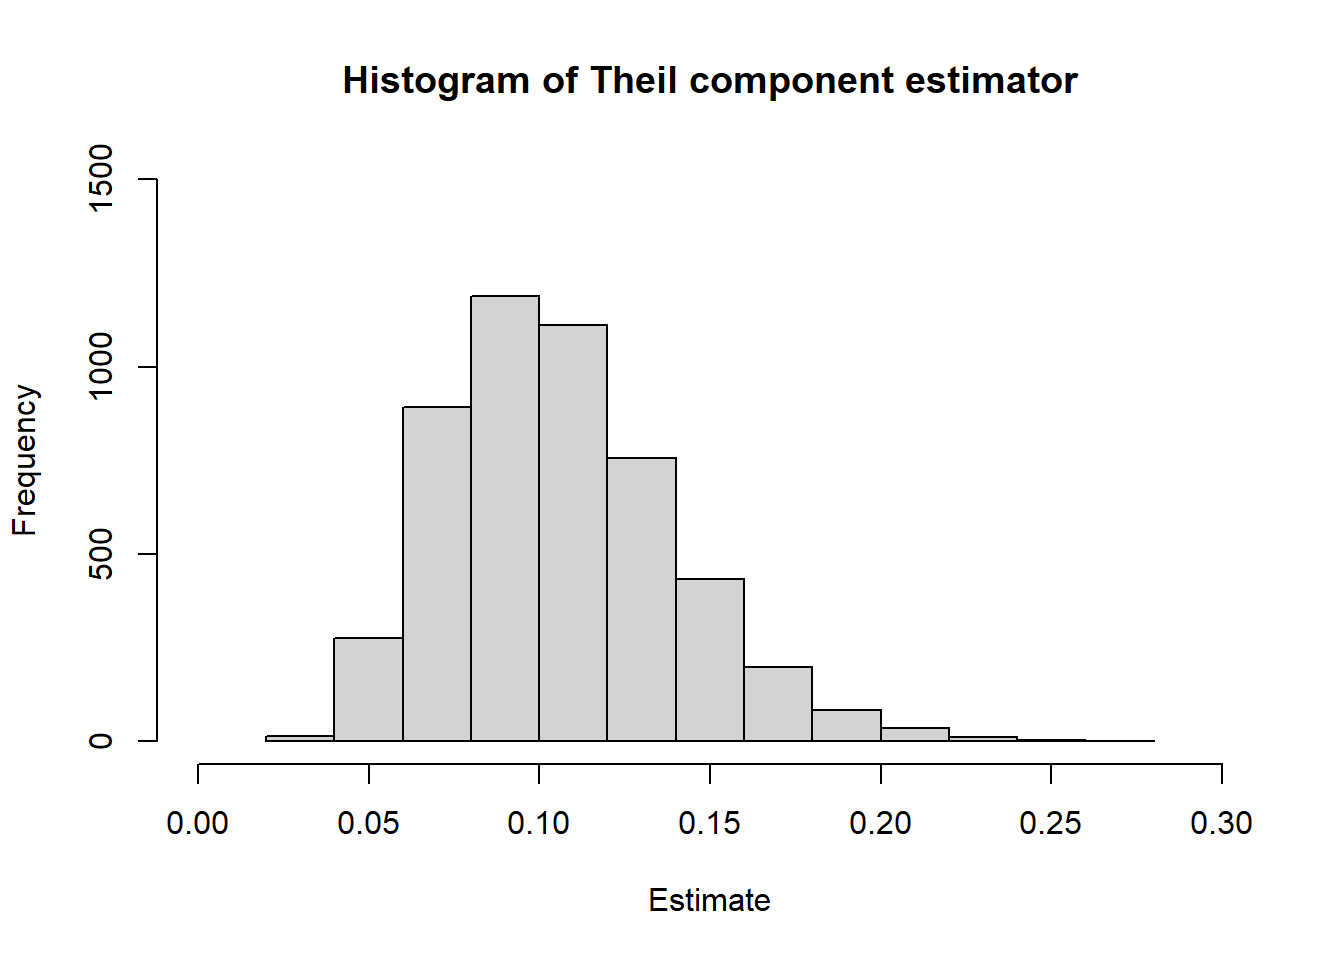
\includegraphics{context_files/figure-latex/unnamed-chunk-55-1.pdf}

For additional usage examples of \texttt{svywatts} and \texttt{svywattsdec}, type \texttt{?convey::svywatts} or \texttt{?convey::svywattsdec} in the R console.

\hypertarget{inequality}{%
\chapter{Inequality Measurement}\label{inequality}}

Another problem faced by societies is inequality. Economic inequality can have several different meanings, including (but not limited to) income, education, resources, opportunities, and well-being. Usually, studies on economic inequality focus on income distribution.

Most inequality data comes from censuses and household surveys. Therefore, in order to produce reliable estimates from survey data, procedures that account for complex sampling designs are necessary.

This chapter presents the inequality measures available in the \texttt{convey} library with replication examples where possible. It starts with an attempt to measure inequality between two groups of a population, then summarizes the general idea of inequality indices by discussing techniques like the quintile share ratio, the Lorenz curve, and the commonly-used Gini coefficient. Next, this chapter discusses the concept of entropy and presents inequality measures (and their decompositions) based on that method. This chapter concludes with a discussion regarding the tradeoffs of selecting among the various inequality measures.

\hypertarget{the-gender-pay-gap-svygpg}{%
\section{The Gender Pay Gap (svygpg)}\label{the-gender-pay-gap-svygpg}}

Although the Gender Pay Gap (GPG) is not an inequality measure in the usual sense, it can still be a useful instrument to evaluate the effects of gender discrimination. Put simply, it expresses the relative difference between the average hourly earnings of men and women, presenting this difference as a percentage of the average of hourly earnings of men. Like some other functions described in this text, the GPG can also be calculated using wealth or assets in place of earnings.

In mathematical terms, this index can be described as,

\[ GPG = \frac{ \bar{y}_{male} - \bar{y}_{female} }{ \bar{y}_{male} } \]

As we can see from the formula, if there is no difference among classes, \(GPG = 0\). Else, if \(GPG > 0\), it means that the average hourly income received by women are \(GPG\) percent smaller than men's. For negative \(GPG\), it means that women's hourly earnings are \(GPG\) percent larger than men's. In other words, the larger the \(GPG\), larger is the shortfall of women's hourly earnings.

We can also develop a more straightforward idea: for every \$1 raise in men's hourly earnings, women's hourly earnings are expected to increase \$\((1-GPG)\). For instance, assuming \(GPG = 0.8\), for every \$1.00 increase in men's average hourly earnings, women's hourly earnings would increase only \$0.20.

The details of the linearization of the GPG are discussed by \textcite{deville1999} and \textcite{osier2009}.

\begin{center}\rule{0.5\linewidth}{0.5pt}\end{center}

\textbf{A replication example}

The R \texttt{vardpoor} package \autocite{vardpoor}, created by researchers at the Central Statistical Bureau of Latvia, includes a GPG coefficient calculation using the ultimate cluster method. The example below reproduces those statistics.

Load and prepare the same data set:

\begin{Shaded}
\begin{Highlighting}[]
\CommentTok{\# load the convey package}
\FunctionTok{library}\NormalTok{(convey)}

\CommentTok{\# load the survey library}
\FunctionTok{library}\NormalTok{(survey)}

\CommentTok{\# load the vardpoor library}
\FunctionTok{library}\NormalTok{(vardpoor)}

\CommentTok{\# load the laeken library}
\FunctionTok{library}\NormalTok{(laeken)}

\CommentTok{\# load the synthetic EU statistics on income \& living conditions}
\FunctionTok{data}\NormalTok{(eusilc)}

\CommentTok{\# make all column names lowercase}
\FunctionTok{names}\NormalTok{(eusilc) }\OtherTok{\textless{}{-}} \FunctionTok{tolower}\NormalTok{(}\FunctionTok{names}\NormalTok{(eusilc))}

\CommentTok{\# coerce the gender variable to numeric 1 or 2}
\NormalTok{eusilc}\SpecialCharTok{$}\NormalTok{one\_two }\OtherTok{\textless{}{-}} \FunctionTok{as.numeric}\NormalTok{(eusilc}\SpecialCharTok{$}\NormalTok{rb090 }\SpecialCharTok{==} \StringTok{"female"}\NormalTok{) }\SpecialCharTok{+} \DecValTok{1}

\CommentTok{\# add a column with the row number}
\NormalTok{dati }\OtherTok{\textless{}{-}}\NormalTok{ data.table}\SpecialCharTok{::}\FunctionTok{data.table}\NormalTok{(}\AttributeTok{IDd =} \DecValTok{1}\SpecialCharTok{:}\FunctionTok{nrow}\NormalTok{(eusilc), eusilc)}

\CommentTok{\# calculate the gpg coefficient}
\CommentTok{\# using the R vardpoor library}
\NormalTok{varpoord\_gpg\_calculation }\OtherTok{\textless{}{-}}
  \FunctionTok{varpoord}\NormalTok{(}
    \CommentTok{\# analysis variable}
    \AttributeTok{Y =} \StringTok{"eqincome"}\NormalTok{,}
    
    \CommentTok{\# weights variable}
    \AttributeTok{w\_final =} \StringTok{"rb050"}\NormalTok{,}
    
    \CommentTok{\# row number variable}
    \AttributeTok{ID\_level1 =} \StringTok{"IDd"}\NormalTok{,}
    
    \CommentTok{\# row number variable}
    \AttributeTok{ID\_level2 =} \StringTok{"IDd"}\NormalTok{,}
    
    \CommentTok{\# strata variable}
    \AttributeTok{H =} \StringTok{"db040"}\NormalTok{,}
    
    \AttributeTok{N\_h =} \ConstantTok{NULL}\NormalTok{ ,}
    
    \CommentTok{\# clustering variable}
    \AttributeTok{PSU =} \StringTok{"rb030"}\NormalTok{,}
    
    \CommentTok{\# data.table}
    \AttributeTok{dataset =}\NormalTok{ dati,}
    
    \CommentTok{\# gpg coefficient function}
    \AttributeTok{type =} \StringTok{"lingpg"}\NormalTok{ ,}
    
    \CommentTok{\# gender variable}
    \AttributeTok{gender =} \StringTok{"one\_two"}\NormalTok{,}
    
    \CommentTok{\# get linearized variable}
    \AttributeTok{outp\_lin =} \ConstantTok{TRUE}
\NormalTok{  )}



\CommentTok{\# construct a survey.design}
\CommentTok{\# using our recommended setup}
\NormalTok{des\_eusilc }\OtherTok{\textless{}{-}}
  \FunctionTok{svydesign}\NormalTok{(}
    \AttributeTok{ids =} \SpecialCharTok{\textasciitilde{}}\NormalTok{ rb030 ,}
    \AttributeTok{strata =} \SpecialCharTok{\textasciitilde{}}\NormalTok{ db040 ,}
    \AttributeTok{weights =} \SpecialCharTok{\textasciitilde{}}\NormalTok{ rb050 ,}
    \AttributeTok{data =}\NormalTok{ eusilc}
\NormalTok{  )}

\CommentTok{\# immediately run the convey\_prep function on it}
\NormalTok{des\_eusilc }\OtherTok{\textless{}{-}} \FunctionTok{convey\_prep}\NormalTok{(des\_eusilc)}

\CommentTok{\# coefficients do match}
\NormalTok{varpoord\_gpg\_calculation}\SpecialCharTok{$}\NormalTok{all\_result}\SpecialCharTok{$}\NormalTok{value}
\end{Highlighting}
\end{Shaded}

\begin{verbatim}
## [1] 7.645389
\end{verbatim}

\begin{Shaded}
\begin{Highlighting}[]
\FunctionTok{coef}\NormalTok{(}\FunctionTok{svygpg}\NormalTok{( }\SpecialCharTok{\textasciitilde{}}\NormalTok{ eqincome , des\_eusilc , }\AttributeTok{sex =} \SpecialCharTok{\textasciitilde{}}\NormalTok{ rb090)) }\SpecialCharTok{*} \DecValTok{100}
\end{Highlighting}
\end{Shaded}

\begin{verbatim}
##  eqincome 
## -8.278297
\end{verbatim}

\begin{Shaded}
\begin{Highlighting}[]
\CommentTok{\# linearized variables do match}
\CommentTok{\# vardpoor}
\NormalTok{lin\_gpg\_varpoord }\OtherTok{\textless{}{-}}\NormalTok{ varpoord\_gpg\_calculation}\SpecialCharTok{$}\NormalTok{lin\_out}\SpecialCharTok{$}\NormalTok{lin\_gpg}
\CommentTok{\# convey}
\NormalTok{lin\_gpg\_convey }\OtherTok{\textless{}{-}}
  \FunctionTok{attr}\NormalTok{(}\FunctionTok{svygpg}\NormalTok{( }\SpecialCharTok{\textasciitilde{}}\NormalTok{ eqincome , des\_eusilc, }\AttributeTok{sex =} \SpecialCharTok{\textasciitilde{}}\NormalTok{ rb090), }\StringTok{"lin"}\NormalTok{)}

\CommentTok{\# check equality}
\FunctionTok{all.equal}\NormalTok{(lin\_gpg\_varpoord, }\DecValTok{100} \SpecialCharTok{*}\NormalTok{ lin\_gpg\_convey[, }\DecValTok{1}\NormalTok{])}
\end{Highlighting}
\end{Shaded}

\begin{verbatim}
## [1] "Mean relative difference: 2.172419"
\end{verbatim}

\begin{Shaded}
\begin{Highlighting}[]
\CommentTok{\# variances do not match exactly}
\FunctionTok{attr}\NormalTok{(}\FunctionTok{svygpg}\NormalTok{( }\SpecialCharTok{\textasciitilde{}}\NormalTok{ eqincome , des\_eusilc , }\AttributeTok{sex =} \SpecialCharTok{\textasciitilde{}}\NormalTok{ rb090) , }\StringTok{\textquotesingle{}var\textquotesingle{}}\NormalTok{) }\SpecialCharTok{*} \DecValTok{10000}
\end{Highlighting}
\end{Shaded}

\begin{verbatim}
##           eqincome
## eqincome 0.8926311
\end{verbatim}

\begin{Shaded}
\begin{Highlighting}[]
\NormalTok{varpoord\_gpg\_calculation}\SpecialCharTok{$}\NormalTok{all\_result}\SpecialCharTok{$}\NormalTok{var}
\end{Highlighting}
\end{Shaded}

\begin{verbatim}
## [1] 0.6482346
\end{verbatim}

\begin{Shaded}
\begin{Highlighting}[]
\CommentTok{\# standard errors do not match exactly}
\NormalTok{varpoord\_gpg\_calculation}\SpecialCharTok{$}\NormalTok{all\_result}\SpecialCharTok{$}\NormalTok{se}
\end{Highlighting}
\end{Shaded}

\begin{verbatim}
## [1] 0.8051301
\end{verbatim}

\begin{Shaded}
\begin{Highlighting}[]
\FunctionTok{SE}\NormalTok{(}\FunctionTok{svygpg}\NormalTok{( }\SpecialCharTok{\textasciitilde{}}\NormalTok{ eqincome , des\_eusilc , }\AttributeTok{sex =} \SpecialCharTok{\textasciitilde{}}\NormalTok{ rb090)) }\SpecialCharTok{*} \DecValTok{100}
\end{Highlighting}
\end{Shaded}

\begin{verbatim}
##           eqincome
## eqincome 0.9447916
\end{verbatim}

The variance estimate is computed by using the approximation defined in \ref{var}, while the linearized variable \(z\) is defined by \ref{lin}. The functions \texttt{convey::svygpg} and \texttt{vardpoor::lingpg} produce the same linearized variable \(z\).

However, the measures of uncertainty do not line up, because \texttt{library(vardpoor)} defaults to an ultimate cluster method that can be replicated with an alternative setup of the \texttt{survey.design} object.

\begin{Shaded}
\begin{Highlighting}[]
\CommentTok{\# within each strata, sum up the weights}
\NormalTok{cluster\_sums }\OtherTok{\textless{}{-}}
  \FunctionTok{aggregate}\NormalTok{(eusilc}\SpecialCharTok{$}\NormalTok{rb050 , }\FunctionTok{list}\NormalTok{(eusilc}\SpecialCharTok{$}\NormalTok{db040) , sum)}

\CommentTok{\# name the within{-}strata sums of weights the \textasciigrave{}cluster\_sum\textasciigrave{}}
\FunctionTok{names}\NormalTok{(cluster\_sums) }\OtherTok{\textless{}{-}} \FunctionTok{c}\NormalTok{(}\StringTok{"db040"}\NormalTok{ , }\StringTok{"cluster\_sum"}\NormalTok{)}

\CommentTok{\# merge this column back onto the data.frame}
\NormalTok{eusilc }\OtherTok{\textless{}{-}} \FunctionTok{merge}\NormalTok{(eusilc , cluster\_sums)}

\CommentTok{\# construct a survey.design}
\CommentTok{\# with the fpc using the cluster sum}
\NormalTok{des\_eusilc\_ultimate\_cluster }\OtherTok{\textless{}{-}}
  \FunctionTok{svydesign}\NormalTok{(}
    \AttributeTok{ids =} \SpecialCharTok{\textasciitilde{}}\NormalTok{ rb030 ,}
    \AttributeTok{strata =} \SpecialCharTok{\textasciitilde{}}\NormalTok{ db040 ,}
    \AttributeTok{weights =} \SpecialCharTok{\textasciitilde{}}\NormalTok{ rb050 ,}
    \AttributeTok{data =}\NormalTok{ eusilc ,}
    \AttributeTok{fpc =} \SpecialCharTok{\textasciitilde{}}\NormalTok{ cluster\_sum}
\NormalTok{  )}

\CommentTok{\# again, immediately run the convey\_prep function on the \textasciigrave{}survey.design\textasciigrave{}}
\NormalTok{des\_eusilc\_ultimate\_cluster }\OtherTok{\textless{}{-}}
  \FunctionTok{convey\_prep}\NormalTok{(des\_eusilc\_ultimate\_cluster)}

\CommentTok{\# matches}
\FunctionTok{attr}\NormalTok{(}\FunctionTok{svygpg}\NormalTok{( }\SpecialCharTok{\textasciitilde{}}\NormalTok{ eqincome , des\_eusilc\_ultimate\_cluster , }\AttributeTok{sex =} \SpecialCharTok{\textasciitilde{}}\NormalTok{ rb090) ,}
     \StringTok{\textquotesingle{}var\textquotesingle{}}\NormalTok{) }\SpecialCharTok{*} \DecValTok{10000}
\end{Highlighting}
\end{Shaded}

\begin{verbatim}
##           eqincome
## eqincome 0.8910413
\end{verbatim}

\begin{Shaded}
\begin{Highlighting}[]
\NormalTok{varpoord\_gpg\_calculation}\SpecialCharTok{$}\NormalTok{all\_result}\SpecialCharTok{$}\NormalTok{var}
\end{Highlighting}
\end{Shaded}

\begin{verbatim}
## [1] 0.6482346
\end{verbatim}

\begin{Shaded}
\begin{Highlighting}[]
\CommentTok{\# matches}
\NormalTok{varpoord\_gpg\_calculation}\SpecialCharTok{$}\NormalTok{all\_result}\SpecialCharTok{$}\NormalTok{se}
\end{Highlighting}
\end{Shaded}

\begin{verbatim}
## [1] 0.8051301
\end{verbatim}

\begin{Shaded}
\begin{Highlighting}[]
\FunctionTok{SE}\NormalTok{(}\FunctionTok{svygpg}\NormalTok{( }\SpecialCharTok{\textasciitilde{}}\NormalTok{ eqincome , des\_eusilc\_ultimate\_cluster , }\AttributeTok{sex =} \SpecialCharTok{\textasciitilde{}}\NormalTok{ rb090)) }\SpecialCharTok{*} \DecValTok{100}
\end{Highlighting}
\end{Shaded}

\begin{verbatim}
##           eqincome
## eqincome 0.9439499
\end{verbatim}

For additional usage examples of \texttt{svygpg}, type \texttt{?convey::svygpg} in the R console.

\hypertarget{quintile-share-ratio-svyqsr}{%
\section{Quintile Share Ratio (svyqsr)}\label{quintile-share-ratio-svyqsr}}

Unlike the previous measure, the Quintile Share Ratio (QSR) is an inequality measure in itself, depending only on the income distribution to evaluate the degree of inequality. By definition, it can be described as the ratio between the income share held by the richest 20\% and the poorest 20\% of the population.

In plain terms, it expresses how many times the wealthier part of the population are richer than the poorest part. For instance, a \(QSR = 4\) implies that the upper class takes home 4 times as much of the total income as the poor.

The QSR can be modified to a more general function of percentile share ratios. For instance, \textcite{cobham2015} argues for using the Palma index, defined as the ratio between the share of the 10\% richest over the share held by the poorest 40\%. There are actually two ways to compute the Palma ratio with the \texttt{convey} package. One is using \texttt{convey::svyqsr} and the other is using \texttt{convey::svylorenz} - they won't match exactly because of different estimators, but are asymptotically equal. Since the Palma ratio is the top 10\% divided by the bottom 40\%, in \texttt{convey::svyqsr} this could be achieved using \texttt{alpha1\ =\ .40} and \texttt{alpha2\ =\ .90}. Note that the \texttt{vardpoor::linqsr} function only accepts a single \texttt{alpha} parameter (defaulting to \texttt{0.2} and \texttt{1\ -\ 0.2}), meaning the Palma index cannot presently be computed using that function.

The details of the linearization of the QSR are discussed by \textcite{deville1999} and \textcite{osier2009}.

\begin{center}\rule{0.5\linewidth}{0.5pt}\end{center}

\textbf{A replication example}

The R \texttt{vardpoor} package \autocite{vardpoor}, created by researchers at the Central Statistical Bureau of Latvia, includes a QSR coefficient calculation using the ultimate cluster method. The example below reproduces those statistics.

Load and prepare the same data set:

\begin{Shaded}
\begin{Highlighting}[]
\CommentTok{\# load the convey package}
\FunctionTok{library}\NormalTok{(convey)}

\CommentTok{\# load the survey library}
\FunctionTok{library}\NormalTok{(survey)}

\CommentTok{\# load the vardpoor library}
\FunctionTok{library}\NormalTok{(vardpoor)}

\CommentTok{\# load the laeken library}
\FunctionTok{library}\NormalTok{(laeken)}

\CommentTok{\# load the synthetic EU statistics on income \& living conditions}
\FunctionTok{data}\NormalTok{(eusilc)}

\CommentTok{\# make all column names lowercase}
\FunctionTok{names}\NormalTok{(eusilc) }\OtherTok{\textless{}{-}} \FunctionTok{tolower}\NormalTok{(}\FunctionTok{names}\NormalTok{(eusilc))}

\CommentTok{\# add a column with the row number}
\NormalTok{dati }\OtherTok{\textless{}{-}}\NormalTok{ data.table}\SpecialCharTok{::}\FunctionTok{data.table}\NormalTok{(}\AttributeTok{IDd =} \DecValTok{1}\SpecialCharTok{:}\FunctionTok{nrow}\NormalTok{(eusilc), eusilc)}

\CommentTok{\# calculate the qsr coefficient}
\CommentTok{\# using the R vardpoor library}
\NormalTok{varpoord\_qsr\_calculation }\OtherTok{\textless{}{-}}
  \FunctionTok{varpoord}\NormalTok{(}
    \CommentTok{\# analysis variable}
    \AttributeTok{Y =} \StringTok{"eqincome"}\NormalTok{,}
    
    \CommentTok{\# weights variable}
    \AttributeTok{w\_final =} \StringTok{"rb050"}\NormalTok{,}
    
    \CommentTok{\# row number variable}
    \AttributeTok{ID\_level1 =} \StringTok{"IDd"}\NormalTok{,}
    
    \CommentTok{\# row number variable}
    \AttributeTok{ID\_level2 =} \StringTok{"IDd"}\NormalTok{,}
    
    \CommentTok{\# strata variable}
    \AttributeTok{H =} \StringTok{"db040"}\NormalTok{,}
    
    \AttributeTok{N\_h =} \ConstantTok{NULL}\NormalTok{ ,}
    
    \CommentTok{\# clustering variable}
    \AttributeTok{PSU =} \StringTok{"rb030"}\NormalTok{,}
    
    \CommentTok{\# data.table}
    \AttributeTok{dataset =}\NormalTok{ dati,}
    
    \CommentTok{\# qsr coefficient function}
    \AttributeTok{type =} \StringTok{"linqsr"}\NormalTok{,}
    
    \CommentTok{\# poverty threshold range}
    \AttributeTok{alpha =} \DecValTok{20}\NormalTok{ ,}
    
    \CommentTok{\# get linearized variable}
    \AttributeTok{outp\_lin =} \ConstantTok{TRUE}
    
\NormalTok{  )}



\CommentTok{\# construct a survey.design}
\CommentTok{\# using our recommended setup}
\NormalTok{des\_eusilc }\OtherTok{\textless{}{-}}
  \FunctionTok{svydesign}\NormalTok{(}
    \AttributeTok{ids =} \SpecialCharTok{\textasciitilde{}}\NormalTok{ rb030 ,}
    \AttributeTok{strata =} \SpecialCharTok{\textasciitilde{}}\NormalTok{ db040 ,}
    \AttributeTok{weights =} \SpecialCharTok{\textasciitilde{}}\NormalTok{ rb050 ,}
    \AttributeTok{data =}\NormalTok{ eusilc}
\NormalTok{  )}

\CommentTok{\# immediately run the convey\_prep function on it}
\NormalTok{des\_eusilc }\OtherTok{\textless{}{-}} \FunctionTok{convey\_prep}\NormalTok{(des\_eusilc)}

\CommentTok{\# coefficients do match}
\NormalTok{varpoord\_qsr\_calculation}\SpecialCharTok{$}\NormalTok{all\_result}\SpecialCharTok{$}\NormalTok{value}
\end{Highlighting}
\end{Shaded}

\begin{verbatim}
## [1] 3.970004
\end{verbatim}

\begin{Shaded}
\begin{Highlighting}[]
\FunctionTok{coef}\NormalTok{(}\FunctionTok{svyqsr}\NormalTok{( }\SpecialCharTok{\textasciitilde{}}\NormalTok{ eqincome , des\_eusilc))}
\end{Highlighting}
\end{Shaded}

\begin{verbatim}
## eqincome 
## 3.970004
\end{verbatim}

\begin{Shaded}
\begin{Highlighting}[]
\CommentTok{\# linearized variables do match}
\CommentTok{\# vardpoor}
\NormalTok{lin\_qsr\_varpoord }\OtherTok{\textless{}{-}}\NormalTok{ varpoord\_qsr\_calculation}\SpecialCharTok{$}\NormalTok{lin\_out}\SpecialCharTok{$}\NormalTok{lin\_qsr}
\CommentTok{\# convey}
\NormalTok{lin\_qsr\_convey }\OtherTok{\textless{}{-}}
  \FunctionTok{as.numeric}\NormalTok{(}\FunctionTok{attr}\NormalTok{(}\FunctionTok{svyqsr}\NormalTok{( }\SpecialCharTok{\textasciitilde{}}\NormalTok{ eqincome ,}
\NormalTok{                          des\_eusilc ,}
                          \AttributeTok{linearized =} \ConstantTok{TRUE}\NormalTok{) ,}
                  \StringTok{"linearized"}\NormalTok{))}

\CommentTok{\# check equality}
\FunctionTok{all.equal}\NormalTok{(lin\_qsr\_varpoord, lin\_qsr\_convey)}
\end{Highlighting}
\end{Shaded}

\begin{verbatim}
## [1] TRUE
\end{verbatim}

\begin{Shaded}
\begin{Highlighting}[]
\CommentTok{\# variances do not match exactly}
\FunctionTok{attr}\NormalTok{(}\FunctionTok{svyqsr}\NormalTok{( }\SpecialCharTok{\textasciitilde{}}\NormalTok{ eqincome , des\_eusilc) , }\StringTok{\textquotesingle{}var\textquotesingle{}}\NormalTok{)}
\end{Highlighting}
\end{Shaded}

\begin{verbatim}
##             eqincome
## eqincome 0.001810537
\end{verbatim}

\begin{Shaded}
\begin{Highlighting}[]
\NormalTok{varpoord\_qsr\_calculation}\SpecialCharTok{$}\NormalTok{all\_result}\SpecialCharTok{$}\NormalTok{var}
\end{Highlighting}
\end{Shaded}

\begin{verbatim}
## [1] 0.001807323
\end{verbatim}

\begin{Shaded}
\begin{Highlighting}[]
\CommentTok{\# standard errors do not match exactly}
\NormalTok{varpoord\_qsr\_calculation}\SpecialCharTok{$}\NormalTok{all\_result}\SpecialCharTok{$}\NormalTok{se}
\end{Highlighting}
\end{Shaded}

\begin{verbatim}
## [1] 0.04251263
\end{verbatim}

\begin{Shaded}
\begin{Highlighting}[]
\FunctionTok{SE}\NormalTok{(}\FunctionTok{svyqsr}\NormalTok{( }\SpecialCharTok{\textasciitilde{}}\NormalTok{ eqincome , des\_eusilc))}
\end{Highlighting}
\end{Shaded}

\begin{verbatim}
##            eqincome
## eqincome 0.04255041
\end{verbatim}

The variance estimate is computed by using the approximation defined in \ref{var}, while the linearized variable \(z\) is defined by \ref{lin}. The functions \texttt{convey::svyqsr} and \texttt{vardpoor::linqsr} produce the same linearized variable \(z\).

However, the measures of uncertainty do not line up, because \texttt{library(vardpoor)} defaults to an ultimate cluster method that can be replicated with an alternative setup of the \texttt{survey.design} object.

\begin{Shaded}
\begin{Highlighting}[]
\CommentTok{\# within each strata, sum up the weights}
\NormalTok{cluster\_sums }\OtherTok{\textless{}{-}}
  \FunctionTok{aggregate}\NormalTok{(eusilc}\SpecialCharTok{$}\NormalTok{rb050 , }\FunctionTok{list}\NormalTok{(eusilc}\SpecialCharTok{$}\NormalTok{db040) , sum)}

\CommentTok{\# name the within{-}strata sums of weights the \textasciigrave{}cluster\_sum\textasciigrave{}}
\FunctionTok{names}\NormalTok{(cluster\_sums) }\OtherTok{\textless{}{-}} \FunctionTok{c}\NormalTok{(}\StringTok{"db040"}\NormalTok{ , }\StringTok{"cluster\_sum"}\NormalTok{)}

\CommentTok{\# merge this column back onto the data.frame}
\NormalTok{eusilc }\OtherTok{\textless{}{-}} \FunctionTok{merge}\NormalTok{(eusilc , cluster\_sums)}

\CommentTok{\# construct a survey.design}
\CommentTok{\# with the fpc using the cluster sum}
\NormalTok{des\_eusilc\_ultimate\_cluster }\OtherTok{\textless{}{-}}
  \FunctionTok{svydesign}\NormalTok{(}
    \AttributeTok{ids =} \SpecialCharTok{\textasciitilde{}}\NormalTok{ rb030 ,}
    \AttributeTok{strata =} \SpecialCharTok{\textasciitilde{}}\NormalTok{ db040 ,}
    \AttributeTok{weights =} \SpecialCharTok{\textasciitilde{}}\NormalTok{ rb050 ,}
    \AttributeTok{data =}\NormalTok{ eusilc ,}
    \AttributeTok{fpc =} \SpecialCharTok{\textasciitilde{}}\NormalTok{ cluster\_sum}
\NormalTok{  )}

\CommentTok{\# again, immediately run the convey\_prep function on the \textasciigrave{}survey.design\textasciigrave{}}
\NormalTok{des\_eusilc\_ultimate\_cluster }\OtherTok{\textless{}{-}}
  \FunctionTok{convey\_prep}\NormalTok{(des\_eusilc\_ultimate\_cluster)}

\CommentTok{\# matches}
\FunctionTok{attr}\NormalTok{(}\FunctionTok{svyqsr}\NormalTok{( }\SpecialCharTok{\textasciitilde{}}\NormalTok{ eqincome , des\_eusilc\_ultimate\_cluster) , }\StringTok{\textquotesingle{}var\textquotesingle{}}\NormalTok{)}
\end{Highlighting}
\end{Shaded}

\begin{verbatim}
##             eqincome
## eqincome 0.001807323
\end{verbatim}

\begin{Shaded}
\begin{Highlighting}[]
\NormalTok{varpoord\_qsr\_calculation}\SpecialCharTok{$}\NormalTok{all\_result}\SpecialCharTok{$}\NormalTok{var}
\end{Highlighting}
\end{Shaded}

\begin{verbatim}
## [1] 0.001807323
\end{verbatim}

\begin{Shaded}
\begin{Highlighting}[]
\CommentTok{\# matches}
\NormalTok{varpoord\_qsr\_calculation}\SpecialCharTok{$}\NormalTok{all\_result}\SpecialCharTok{$}\NormalTok{se}
\end{Highlighting}
\end{Shaded}

\begin{verbatim}
## [1] 0.04251263
\end{verbatim}

\begin{Shaded}
\begin{Highlighting}[]
\FunctionTok{SE}\NormalTok{(}\FunctionTok{svyqsr}\NormalTok{( }\SpecialCharTok{\textasciitilde{}}\NormalTok{ eqincome , des\_eusilc\_ultimate\_cluster))}
\end{Highlighting}
\end{Shaded}

\begin{verbatim}
##            eqincome
## eqincome 0.04251263
\end{verbatim}

For additional usage examples of \texttt{svyqsr}, type \texttt{?convey::svyqsr} in the R console.

\hypertarget{lorenz-curve-svylorenz}{%
\section{Lorenz Curve (svylorenz)}\label{lorenz-curve-svylorenz}}

Though not an inequality measure in itself, the Lorenz curve is a classic instrument of distribution analysis. This function associates a cumulative share of the population to the share of the total income earned. In mathematical terms,

\[
L(p) = \frac{\int_{-\infty}^{Q_p}yf(y)dy}{\int_{-\infty}^{+\infty}yf(y)dy}
\]

where \(Q_p\) is the quantile \(p\) of the population.

The two extreme distributive cases are

\begin{itemize}
\tightlist
\item
  Perfect equality:

  \begin{itemize}
  \tightlist
  \item
    Every individual has the same income;
  \item
    Every share of the population has the same share of the income;
  \item
    Therefore, the reference curve is \[L(p) = p \text{ } \forall p \in [0,1] \text{.}\]
  \end{itemize}
\item
  Perfect inequality:

  \begin{itemize}
  \tightlist
  \item
    One individual concentrates all of society's income, while the other individuals have zero income;
  \item
    Therefore, the reference curve is
  \end{itemize}
\end{itemize}

\[
L(p)=
\begin{cases}
0, &\forall p < 1 \\
1, &\text{if } p = 1 \text{.}
\end{cases}
\]

In order to evaluate the degree of inequality in a society, the analyst looks at the distance between the real curve and those two reference curves.

The estimator of this function was derived by \textcite{kovacevic1997}:

\[
L(p) = \frac{ \sum_{i \in S} w_i \cdot y_i \cdot \delta \{ y_i \le \widehat{Q}_p \}}{\widehat{Y}}, \text{ } 0 \le p \le 1.
\]

Yet, this formula is used to calculate specific points of the curve and their respective SEs. The formula to plot an approximation of the continuous empirical curve comes from \textcite{lerman1989}.

\begin{center}\rule{0.5\linewidth}{0.5pt}\end{center}

\textbf{A replication example}

In October 2016, \autocite{jann2016} released a pre-publication working paper to estimate Lorenz and concentration curves using stata. The example below reproduces the statistics presented in his section 4.1.

\begin{Shaded}
\begin{Highlighting}[]
\CommentTok{\# load the convey package}
\FunctionTok{library}\NormalTok{(convey)}

\CommentTok{\# load the survey library}
\FunctionTok{library}\NormalTok{(survey)}

\CommentTok{\# load the stata{-}style webuse library}
\FunctionTok{library}\NormalTok{(webuse)}

\CommentTok{\# load the NLSW 1988 data}
\FunctionTok{webuse}\NormalTok{(}\StringTok{"nlsw88"}\NormalTok{)}

\CommentTok{\# coerce that \textasciigrave{}tbl\_df\textasciigrave{} to a standard R \textasciigrave{}data.frame\textasciigrave{}}
\NormalTok{nlsw88 }\OtherTok{\textless{}{-}} \FunctionTok{data.frame}\NormalTok{(nlsw88)}

\CommentTok{\# initiate a linearized survey design object}
\NormalTok{des\_nlsw88 }\OtherTok{\textless{}{-}} \FunctionTok{svydesign}\NormalTok{(}\AttributeTok{ids =} \SpecialCharTok{\textasciitilde{}} \DecValTok{1}\NormalTok{ , }\AttributeTok{data =}\NormalTok{ nlsw88)}
\end{Highlighting}
\end{Shaded}

\begin{verbatim}
## Warning in svydesign.default(ids = ~1, data = nlsw88): No weights or
## probabilities supplied, assuming equal probability
\end{verbatim}

\begin{Shaded}
\begin{Highlighting}[]
\CommentTok{\# immediately run the \textasciigrave{}convey\_prep\textasciigrave{} function on the survey design}
\NormalTok{des\_nlsw88 }\OtherTok{\textless{}{-}} \FunctionTok{convey\_prep}\NormalTok{(des\_nlsw88)}

\CommentTok{\# estimates lorenz curve}
\NormalTok{result.lin }\OtherTok{\textless{}{-}}
  \FunctionTok{svylorenz}\NormalTok{( }\SpecialCharTok{\textasciitilde{}}\NormalTok{ wage,}
\NormalTok{             des\_nlsw88,}
             \AttributeTok{quantiles =} \FunctionTok{seq}\NormalTok{(}\DecValTok{0}\NormalTok{, }\DecValTok{1}\NormalTok{, .}\DecValTok{05}\NormalTok{),}
             \AttributeTok{na.rm =} \ConstantTok{TRUE}\NormalTok{)}
\end{Highlighting}
\end{Shaded}

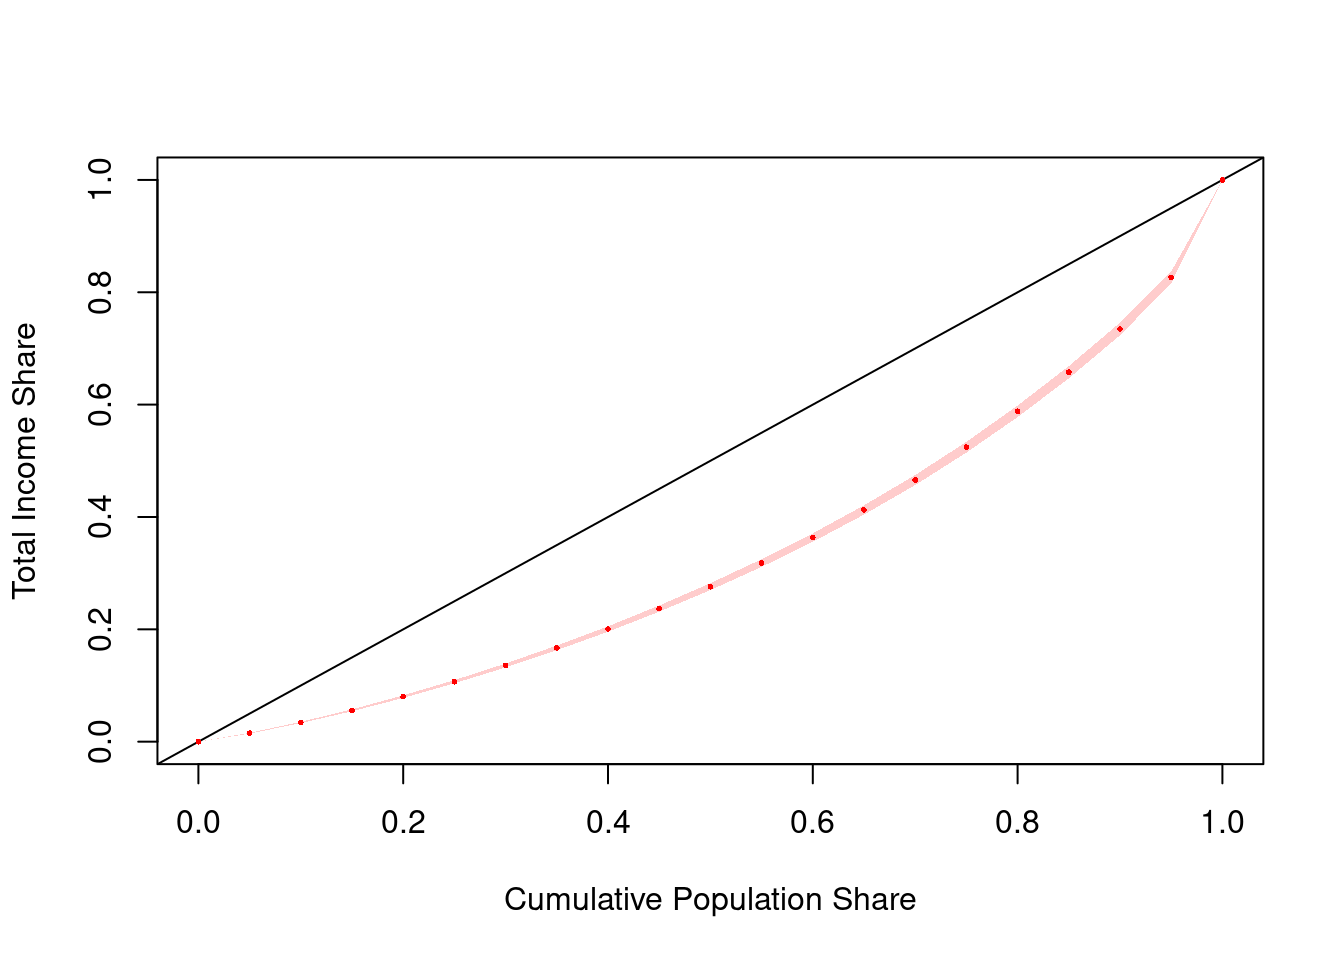
\includegraphics{context_files/figure-latex/unnamed-chunk-60-1.pdf}

\begin{Shaded}
\begin{Highlighting}[]
\CommentTok{\# note: most survey commands in R use Inf degrees of freedom by default}
\CommentTok{\# stata generally uses the degrees of freedom of the survey design.}
\CommentTok{\# therefore, while the degf() parameters passed to qt()}
\CommentTok{\# serve to prove a precise replication of stata,}
\CommentTok{\# it is generally not necessary}
\NormalTok{section\_four\_one }\OtherTok{\textless{}{-}}
  \FunctionTok{data.frame}\NormalTok{(}
    \AttributeTok{estimate =} \FunctionTok{coef}\NormalTok{(result.lin) ,}
    \AttributeTok{standard\_error =} \FunctionTok{SE}\NormalTok{(result.lin) ,}
    \AttributeTok{ci\_lower\_bound =}
      \FunctionTok{coef}\NormalTok{(result.lin) }\SpecialCharTok{+}
      \FunctionTok{SE}\NormalTok{(result.lin) }\SpecialCharTok{*}
      \FunctionTok{qt}\NormalTok{(}\FloatTok{0.025}\NormalTok{ , }\FunctionTok{degf}\NormalTok{(}\FunctionTok{subset}\NormalTok{(}
\NormalTok{        des\_nlsw88 , }\SpecialCharTok{!}\FunctionTok{is.na}\NormalTok{(wage)}
\NormalTok{      ))) ,}
    \AttributeTok{ci\_upper\_bound =}
      \FunctionTok{coef}\NormalTok{(result.lin) }\SpecialCharTok{+}
      \FunctionTok{SE}\NormalTok{(result.lin) }\SpecialCharTok{*}
      \FunctionTok{qt}\NormalTok{(}\FloatTok{0.975}\NormalTok{ , }\FunctionTok{degf}\NormalTok{(}\FunctionTok{subset}\NormalTok{(}
\NormalTok{        des\_nlsw88 , }\SpecialCharTok{!}\FunctionTok{is.na}\NormalTok{(wage)}
\NormalTok{      )))}
\NormalTok{  )}
\end{Highlighting}
\end{Shaded}

\begin{tabular}{lrrrr}
\toprule
  & estimate & standard\_error & ci\_lower\_bound & ci\_upper\_bound\\
\midrule
L(0) & 0.0000000 & 0.0000000 & 0.0000000 & 0.0000000\\
L(0.05) & 0.0151060 & 0.0004159 & 0.0142904 & 0.0159216\\
L(0.1) & 0.0342651 & 0.0007021 & 0.0328882 & 0.0356420\\
L(0.15) & 0.0558635 & 0.0010096 & 0.0538836 & 0.0578434\\
L(0.2) & 0.0801846 & 0.0014032 & 0.0774329 & 0.0829363\\
\addlinespace
L(0.25) & 0.1067687 & 0.0017315 & 0.1033732 & 0.1101642\\
L(0.3) & 0.1356307 & 0.0021301 & 0.1314535 & 0.1398078\\
L(0.35) & 0.1670287 & 0.0025182 & 0.1620903 & 0.1719670\\
L(0.4) & 0.2005501 & 0.0029161 & 0.1948315 & 0.2062687\\
L(0.45) & 0.2369209 & 0.0033267 & 0.2303971 & 0.2434447\\
\addlinespace
L(0.5) & 0.2759734 & 0.0037423 & 0.2686347 & 0.2833121\\
L(0.55) & 0.3180215 & 0.0041626 & 0.3098585 & 0.3261844\\
L(0.6) & 0.3633071 & 0.0045833 & 0.3543192 & 0.3722950\\
L(0.65) & 0.4125183 & 0.0050056 & 0.4027021 & 0.4223345\\
L(0.7) & 0.4657641 & 0.0054137 & 0.4551478 & 0.4763804\\
\addlinespace
L(0.75) & 0.5241784 & 0.0058003 & 0.5128039 & 0.5355529\\
L(0.8) & 0.5880894 & 0.0062464 & 0.5758401 & 0.6003388\\
L(0.85) & 0.6577051 & 0.0066148 & 0.6447333 & 0.6706769\\
L(0.9) & 0.7346412 & 0.0068289 & 0.7212497 & 0.7480328\\
L(0.95) & 0.8265786 & 0.0062686 & 0.8142857 & 0.8388715\\
\addlinespace
L(1) & 1.0000000 & 0.0000000 & 1.0000000 & 1.0000000\\
\bottomrule
\end{tabular}

For additional usage examples of \texttt{svylorenz}, type \texttt{?convey::svylorenz} in the R console.

\hypertarget{gini-index-svygini}{%
\section{Gini index (svygini)}\label{gini-index-svygini}}

The Gini index (or Gini coefficient) is an attempt to express the inequality presented in the Lorenz curve as a single number. In essence, it is twice the area between the equality curve and the real Lorenz curve. Put simply:

\[
\begin{aligned}
G &= 2 \bigg( \int_{0}^{1} pdp - \int_{0}^{1} L(p)dp \bigg) \\
\therefore G &= 1 - 2 \int_{0}^{1} L(p)dp
\end{aligned}
\]

where \(G=0\) in case of perfect equality and \(G = 1\) in the case of perfect inequality.

The estimator proposed by \textcite{osier2009} is defined as:

\[
\widehat{G} = \frac{ 2 \sum_{i \in S} w_i r_i y_i - \sum_{i \in S} w_i y_i }{ \hat{Y} }
\]

The linearized formula of \(\widehat{G}\) is used to calculate the SE.

\begin{center}\rule{0.5\linewidth}{0.5pt}\end{center}

\textbf{A replication example}

The R \texttt{vardpoor} package \autocite{vardpoor}, created by researchers at the Central Statistical Bureau of Latvia, includes a Gini coefficient calculation using the ultimate cluster method. The example below reproduces those statistics.

Load and prepare the same data set:

\begin{Shaded}
\begin{Highlighting}[]
\CommentTok{\# load the convey package}
\FunctionTok{library}\NormalTok{(convey)}

\CommentTok{\# load the survey library}
\FunctionTok{library}\NormalTok{(survey)}

\CommentTok{\# load the vardpoor library}
\FunctionTok{library}\NormalTok{(vardpoor)}

\CommentTok{\# load the laeken library}
\FunctionTok{library}\NormalTok{(laeken)}

\CommentTok{\# load the synthetic EU statistics on income \& living conditions}
\FunctionTok{data}\NormalTok{(eusilc)}

\CommentTok{\# make all column names lowercase}
\FunctionTok{names}\NormalTok{(eusilc) }\OtherTok{\textless{}{-}} \FunctionTok{tolower}\NormalTok{(}\FunctionTok{names}\NormalTok{(eusilc))}

\CommentTok{\# add a column with the row number}
\NormalTok{dati }\OtherTok{\textless{}{-}}\NormalTok{ data.table}\SpecialCharTok{::}\FunctionTok{data.table}\NormalTok{(}\AttributeTok{IDd =} \DecValTok{1}\SpecialCharTok{:}\FunctionTok{nrow}\NormalTok{(eusilc), eusilc)}

\CommentTok{\# calculate the gini coefficient}
\CommentTok{\# using the R vardpoor library}
\NormalTok{varpoord\_gini\_calculation }\OtherTok{\textless{}{-}}
  \FunctionTok{varpoord}\NormalTok{(}
    \CommentTok{\# analysis variable}
    \AttributeTok{Y =} \StringTok{"eqincome"}\NormalTok{,}
    
    \CommentTok{\# weights variable}
    \AttributeTok{w\_final =} \StringTok{"rb050"}\NormalTok{,}
    
    \CommentTok{\# row number variable}
    \AttributeTok{ID\_level1 =} \StringTok{"IDd"}\NormalTok{,}
    
    \CommentTok{\# row number variable}
    \AttributeTok{ID\_level2 =} \StringTok{"IDd"}\NormalTok{,}
    
    \CommentTok{\# strata variable}
    \AttributeTok{H =} \StringTok{"db040"}\NormalTok{,}
    
    \AttributeTok{N\_h =} \ConstantTok{NULL}\NormalTok{ ,}
    
    \CommentTok{\# clustering variable}
    \AttributeTok{PSU =} \StringTok{"rb030"}\NormalTok{,}
    
    \CommentTok{\# data.table}
    \AttributeTok{dataset =}\NormalTok{ dati,}
    
    \CommentTok{\# gini coefficient function}
    \AttributeTok{type =} \StringTok{"lingini"}\NormalTok{,}
    
    \CommentTok{\# get linearized variable}
    \AttributeTok{outp\_lin =} \ConstantTok{TRUE}
    
\NormalTok{  )}



\CommentTok{\# construct a survey.design}
\CommentTok{\# using our recommended setup}
\NormalTok{des\_eusilc }\OtherTok{\textless{}{-}}
  \FunctionTok{svydesign}\NormalTok{(}
    \AttributeTok{ids =} \SpecialCharTok{\textasciitilde{}}\NormalTok{ rb030 ,}
    \AttributeTok{strata =} \SpecialCharTok{\textasciitilde{}}\NormalTok{ db040 ,}
    \AttributeTok{weights =} \SpecialCharTok{\textasciitilde{}}\NormalTok{ rb050 ,}
    \AttributeTok{data =}\NormalTok{ eusilc}
\NormalTok{  )}

\CommentTok{\# immediately run the convey\_prep function on it}
\NormalTok{des\_eusilc }\OtherTok{\textless{}{-}} \FunctionTok{convey\_prep}\NormalTok{(des\_eusilc)}

\CommentTok{\# coefficients do match}
\NormalTok{varpoord\_gini\_calculation}\SpecialCharTok{$}\NormalTok{all\_result}\SpecialCharTok{$}\NormalTok{value}
\end{Highlighting}
\end{Shaded}

\begin{verbatim}
## [1] 26.49652
\end{verbatim}

\begin{Shaded}
\begin{Highlighting}[]
\FunctionTok{coef}\NormalTok{(}\FunctionTok{svygini}\NormalTok{( }\SpecialCharTok{\textasciitilde{}}\NormalTok{ eqincome , des\_eusilc)) }\SpecialCharTok{*} \DecValTok{100}
\end{Highlighting}
\end{Shaded}

\begin{verbatim}
## eqincome 
## 26.49652
\end{verbatim}

\begin{Shaded}
\begin{Highlighting}[]
\CommentTok{\# linearized variables do match}
\CommentTok{\# varpoord}
\NormalTok{lin\_gini\_varpoord }\OtherTok{\textless{}{-}}\NormalTok{ varpoord\_gini\_calculation}\SpecialCharTok{$}\NormalTok{lin\_out}\SpecialCharTok{$}\NormalTok{lin\_gini}
\CommentTok{\# convey}
\NormalTok{lin\_gini\_convey }\OtherTok{\textless{}{-}}
  \FunctionTok{attr}\NormalTok{(}\FunctionTok{svygini}\NormalTok{( }\SpecialCharTok{\textasciitilde{}}\NormalTok{ eqincome , des\_eusilc , }\AttributeTok{linearized =} \ConstantTok{TRUE}\NormalTok{) , }\StringTok{"linearized"}\NormalTok{)}

\CommentTok{\# check equality}
\FunctionTok{all.equal}\NormalTok{(lin\_gini\_varpoord , (}\DecValTok{100} \SpecialCharTok{*} \FunctionTok{as.numeric}\NormalTok{(lin\_gini\_convey)))}
\end{Highlighting}
\end{Shaded}

\begin{verbatim}
## [1] TRUE
\end{verbatim}

\begin{Shaded}
\begin{Highlighting}[]
\CommentTok{\# variances do not match exactly}
\FunctionTok{attr}\NormalTok{(}\FunctionTok{svygini}\NormalTok{( }\SpecialCharTok{\textasciitilde{}}\NormalTok{ eqincome , des\_eusilc) , }\StringTok{\textquotesingle{}var\textquotesingle{}}\NormalTok{) }\SpecialCharTok{*} \DecValTok{10000}
\end{Highlighting}
\end{Shaded}

\begin{verbatim}
##            eqincome
## eqincome 0.03790739
\end{verbatim}

\begin{Shaded}
\begin{Highlighting}[]
\NormalTok{varpoord\_gini\_calculation}\SpecialCharTok{$}\NormalTok{all\_result}\SpecialCharTok{$}\NormalTok{var}
\end{Highlighting}
\end{Shaded}

\begin{verbatim}
## [1] 0.03783931
\end{verbatim}

\begin{Shaded}
\begin{Highlighting}[]
\CommentTok{\# standard errors do not match exactly}
\NormalTok{varpoord\_gini\_calculation}\SpecialCharTok{$}\NormalTok{all\_result}\SpecialCharTok{$}\NormalTok{se}
\end{Highlighting}
\end{Shaded}

\begin{verbatim}
## [1] 0.1945233
\end{verbatim}

\begin{Shaded}
\begin{Highlighting}[]
\FunctionTok{SE}\NormalTok{(}\FunctionTok{svygini}\NormalTok{( }\SpecialCharTok{\textasciitilde{}}\NormalTok{ eqincome , des\_eusilc)) }\SpecialCharTok{*} \DecValTok{100}
\end{Highlighting}
\end{Shaded}

\begin{verbatim}
##           eqincome
## eqincome 0.1946982
\end{verbatim}

The variance estimate is computed by using the approximation defined in \ref{var}, while the linearized variable \(z\) is defined by \ref{lin}. The functions \texttt{convey::svygini} and \texttt{vardpoor::lingini} produce the same linearized variable \(z\).

However, the measures of uncertainty do not line up, because \texttt{library(vardpoor)} defaults to an ultimate cluster method that can be replicated with an alternative setup of the \texttt{survey.design} object.

\begin{Shaded}
\begin{Highlighting}[]
\CommentTok{\# within each strata, sum up the weights}
\NormalTok{cluster\_sums }\OtherTok{\textless{}{-}}
  \FunctionTok{aggregate}\NormalTok{(eusilc}\SpecialCharTok{$}\NormalTok{rb050 , }\FunctionTok{list}\NormalTok{(eusilc}\SpecialCharTok{$}\NormalTok{db040) , sum)}

\CommentTok{\# name the within{-}strata sums of weights the \textasciigrave{}cluster\_sum\textasciigrave{}}
\FunctionTok{names}\NormalTok{(cluster\_sums) }\OtherTok{\textless{}{-}} \FunctionTok{c}\NormalTok{(}\StringTok{"db040"}\NormalTok{ , }\StringTok{"cluster\_sum"}\NormalTok{)}

\CommentTok{\# merge this column back onto the data.frame}
\NormalTok{eusilc }\OtherTok{\textless{}{-}} \FunctionTok{merge}\NormalTok{(eusilc , cluster\_sums)}

\CommentTok{\# construct a survey.design}
\CommentTok{\# with the fpc using the cluster sum}
\NormalTok{des\_eusilc\_ultimate\_cluster }\OtherTok{\textless{}{-}}
  \FunctionTok{svydesign}\NormalTok{(}
    \AttributeTok{ids =} \SpecialCharTok{\textasciitilde{}}\NormalTok{ rb030 ,}
    \AttributeTok{strata =} \SpecialCharTok{\textasciitilde{}}\NormalTok{ db040 ,}
    \AttributeTok{weights =} \SpecialCharTok{\textasciitilde{}}\NormalTok{ rb050 ,}
    \AttributeTok{data =}\NormalTok{ eusilc ,}
    \AttributeTok{fpc =} \SpecialCharTok{\textasciitilde{}}\NormalTok{ cluster\_sum}
\NormalTok{  )}

\CommentTok{\# again, immediately run the convey\_prep function on the \textasciigrave{}survey.design\textasciigrave{}}
\NormalTok{des\_eusilc\_ultimate\_cluster }\OtherTok{\textless{}{-}}
  \FunctionTok{convey\_prep}\NormalTok{(des\_eusilc\_ultimate\_cluster)}

\CommentTok{\# matches}
\FunctionTok{attr}\NormalTok{(}\FunctionTok{svygini}\NormalTok{( }\SpecialCharTok{\textasciitilde{}}\NormalTok{ eqincome , des\_eusilc\_ultimate\_cluster) , }\StringTok{\textquotesingle{}var\textquotesingle{}}\NormalTok{) }\SpecialCharTok{*} \DecValTok{10000}
\end{Highlighting}
\end{Shaded}

\begin{verbatim}
##            eqincome
## eqincome 0.03783931
\end{verbatim}

\begin{Shaded}
\begin{Highlighting}[]
\NormalTok{varpoord\_gini\_calculation}\SpecialCharTok{$}\NormalTok{all\_result}\SpecialCharTok{$}\NormalTok{var}
\end{Highlighting}
\end{Shaded}

\begin{verbatim}
## [1] 0.03783931
\end{verbatim}

\begin{Shaded}
\begin{Highlighting}[]
\CommentTok{\# matches}
\NormalTok{varpoord\_gini\_calculation}\SpecialCharTok{$}\NormalTok{all\_result}\SpecialCharTok{$}\NormalTok{se}
\end{Highlighting}
\end{Shaded}

\begin{verbatim}
## [1] 0.1945233
\end{verbatim}

\begin{Shaded}
\begin{Highlighting}[]
\FunctionTok{SE}\NormalTok{(}\FunctionTok{svygini}\NormalTok{( }\SpecialCharTok{\textasciitilde{}}\NormalTok{ eqincome , des\_eusilc\_ultimate\_cluster)) }\SpecialCharTok{*} \DecValTok{100}
\end{Highlighting}
\end{Shaded}

\begin{verbatim}
##           eqincome
## eqincome 0.1945233
\end{verbatim}

\hypertarget{zenga-index-svyzenga}{%
\section{Zenga index (svyzenga)}\label{zenga-index-svyzenga}}

Proposed by \textcite{zenga2007}, the Zenga index is another inequality measure related to the Lorenz curve with interesting properties. For continuous populations, it is defined as:

\[
Z = 1 - \int_{0}^{1} \frac{L(p)}{p} \cdot \frac{ 1 - p }{ 1 - L(p) } dp 
\]

In practice, \texttt{convey} uses the \textcite{barabesi2016} estimator, based on the finite population Zenga index, and a variance estimator derived using Deville's \autocite*{deville1999} influence function method.

Alternatively, \textcite{langel2011} uses an estimator based on smoothed quantiles and a variance estimator based on the \textcite{demnati2004} linearization method. However, \textcite{barabesi2016} finds that both estimators behave very similarly.

The intuition behind the Zenga index is based on argument similar to the Quintile Share Ratio or the Palma index. While the QSR and Palma indices are based on ratios of lower and upper shares, the Zenga scores (but not the measure itself!) is the ratio of lower and upper means. The Zenga index is the average of those scores.

For a given p, when the mean income of the poorest is not much smaller than the mean income of the richest, the ratio is close to one, resulting in Z(p) close to zero. However, when the lower mean is much smaller than the upper mean, the ratio goes to 0, resulting in a Z(p) close to one.

Take the mean income of the poorest 20\% of a population: this is the lower mean. The ``complement'' is the mean income of the richest 80\%: this is the upper mean. If the lower mean is \$100 and the upper mean is \$1,000, then the respective point on the Zenga curve would associate the fraction 20\% to 1 - ( \$100 / \$1,000 ) = 0.9. In other words, Z(20\%) = 90\%.

In this case, we took a fixed p = 20\%; however, the full Zenga curve would be computed varying p from 0\% to 100\%. Then, the Zenga index is the integral of this curve in the interval (0,1).

Unlike the relationship between the Gini coefficient and the Lorenz curve, this allows for a more straightforward graphical interpretation (see Figure 1 from \textcite{langel2011}) of the Zenga index. In fact, the Zenga index is the mean of the Y axis of the Zenga coordinates.

According to \textcite{langel2011}, ``the Zenga index is significantly less affected by extreme observations than the Gini index. This is a very important advantage of the Zenga index because inference from income data is often confronted with extreme values''.

\begin{center}\rule{0.5\linewidth}{0.5pt}\end{center}

\textbf{A replication example}

While it is not possible to reproduce the exact results because their simulation includes random sampling, we can replicate a Monte Carlo experiment similar to the one presented by \textcite{barabesi2016} in Table 2.

Load and prepare the data set:

\begin{Shaded}
\begin{Highlighting}[]
\FunctionTok{library}\NormalTok{(convey)}
\FunctionTok{library}\NormalTok{(survey)}
\FunctionTok{library}\NormalTok{(parallel)}

\CommentTok{\# create a temporary file on the local disk}
\NormalTok{tf }\OtherTok{\textless{}{-}} \FunctionTok{tempfile}\NormalTok{()}

\CommentTok{\# store the location of the zip file}
\NormalTok{data\_zip }\OtherTok{\textless{}{-}}
  \StringTok{"https://www.bancaditalia.it/statistiche/tematiche/indagini{-}famiglie{-}imprese/bilanci{-}famiglie/distribuzione{-}microdati/documenti/ind12\_ascii.zip"}

\CommentTok{\# download to the temporary file}
\FunctionTok{download.file}\NormalTok{(data\_zip , tf , }\AttributeTok{mode =} \StringTok{\textquotesingle{}wb\textquotesingle{}}\NormalTok{)}

\CommentTok{\# unzip the contents of the archive to a temporary directory}
\NormalTok{td }\OtherTok{\textless{}{-}} \FunctionTok{file.path}\NormalTok{(}\FunctionTok{tempdir}\NormalTok{() , }\StringTok{"shiw2012"}\NormalTok{)}
\NormalTok{data\_files }\OtherTok{\textless{}{-}} \FunctionTok{unzip}\NormalTok{(tf , }\AttributeTok{exdir =}\NormalTok{ td)}

\CommentTok{\# load the household, consumption and income from SHIW (2012) survey data}
\NormalTok{hhr.df }\OtherTok{\textless{}{-}} \FunctionTok{read.csv}\NormalTok{(}\FunctionTok{grep}\NormalTok{(}\StringTok{"carcom12"}\NormalTok{ , data\_files , }\AttributeTok{value =} \ConstantTok{TRUE}\NormalTok{))}
\NormalTok{cns.df }\OtherTok{\textless{}{-}} \FunctionTok{read.csv}\NormalTok{(}\FunctionTok{grep}\NormalTok{(}\StringTok{"risfam12"}\NormalTok{ , data\_files , }\AttributeTok{value =} \ConstantTok{TRUE}\NormalTok{))}
\NormalTok{inc.df }\OtherTok{\textless{}{-}} \FunctionTok{read.csv}\NormalTok{(}\FunctionTok{grep}\NormalTok{(}\StringTok{"rper12"}\NormalTok{ , data\_files , }\AttributeTok{value =} \ConstantTok{TRUE}\NormalTok{))}

\CommentTok{\# fixes names}
\FunctionTok{colnames}\NormalTok{(cns.df)[}\DecValTok{1}\NormalTok{] }\OtherTok{\textless{}{-}} \FunctionTok{tolower}\NormalTok{(}\FunctionTok{colnames}\NormalTok{(cns.df))[}\DecValTok{1}\NormalTok{]}

\CommentTok{\# household count should be 8151}
\FunctionTok{stopifnot}\NormalTok{(}\FunctionTok{sum}\NormalTok{(}\SpecialCharTok{!}\FunctionTok{duplicated}\NormalTok{(hhr.df}\SpecialCharTok{$}\NormalTok{nquest)) }\SpecialCharTok{==} \DecValTok{8151}\NormalTok{)}

\CommentTok{\# person count should be 20022}
\FunctionTok{stopifnot}\NormalTok{(}\FunctionTok{sum}\NormalTok{(}\SpecialCharTok{!}\FunctionTok{duplicated}\NormalTok{(}\FunctionTok{paste0}\NormalTok{(}
\NormalTok{  hhr.df}\SpecialCharTok{$}\NormalTok{nquest , }\StringTok{"{-}"}\NormalTok{ , hhr.df}\SpecialCharTok{$}\NormalTok{nord}
\NormalTok{))) }\SpecialCharTok{==} \DecValTok{20022}\NormalTok{)}

\CommentTok{\# income recipients: should be 12986}
\FunctionTok{stopifnot}\NormalTok{(}\FunctionTok{sum}\NormalTok{(hhr.df}\SpecialCharTok{$}\NormalTok{PERC) }\SpecialCharTok{==} \DecValTok{12986}\NormalTok{)}

\CommentTok{\# combine household roster and income datasets}
\NormalTok{pop.df }\OtherTok{\textless{}{-}}
  \FunctionTok{merge}\NormalTok{(}
\NormalTok{    hhr.df ,}
\NormalTok{    inc.df ,}
    \AttributeTok{by =} \FunctionTok{c}\NormalTok{(}\StringTok{"nquest"}\NormalTok{ , }\StringTok{"nord"}\NormalTok{) ,}
    \AttributeTok{all.x =} \ConstantTok{TRUE}\NormalTok{ ,}
    \AttributeTok{sort =} \ConstantTok{FALSE}
\NormalTok{  )}

\CommentTok{\# compute household{-}level income}
\NormalTok{hinc.df }\OtherTok{\textless{}{-}}
\NormalTok{  pop.df[pop.df}\SpecialCharTok{$}\NormalTok{PERC }\SpecialCharTok{==} \DecValTok{1}\NormalTok{ ,}
         \FunctionTok{c}\NormalTok{(}\StringTok{"nquest"}\NormalTok{ , }\StringTok{"nord"}\NormalTok{ , }\StringTok{"PERC"}\NormalTok{ , }\StringTok{"Y"}\NormalTok{ , }\StringTok{"YL"}\NormalTok{ , }\StringTok{"YM"}\NormalTok{ , }\StringTok{"YT"}\NormalTok{ , }\StringTok{"YC"}\NormalTok{) ,}
\NormalTok{         drop }\OtherTok{=} \ConstantTok{FALSE}\NormalTok{]}

\NormalTok{hinc.df }\OtherTok{\textless{}{-}}
  \FunctionTok{aggregate}\NormalTok{(}\FunctionTok{rowSums}\NormalTok{(hinc.df[, }\FunctionTok{c}\NormalTok{(}\StringTok{"YL"}\NormalTok{  , }\StringTok{"YM"}\NormalTok{ , }\StringTok{"YT"}\NormalTok{) , }\AttributeTok{drop =} \ConstantTok{FALSE}\NormalTok{]) ,}
            \FunctionTok{list}\NormalTok{(}\StringTok{"nquest"} \OtherTok{=}\NormalTok{ hinc.df}\SpecialCharTok{$}\NormalTok{nquest) ,}
\NormalTok{            sum ,}
            \AttributeTok{na.rm =} \ConstantTok{TRUE}\NormalTok{)}

\NormalTok{pop.df }\OtherTok{\textless{}{-}}
  \FunctionTok{merge}\NormalTok{(pop.df ,}
\NormalTok{        hinc.df ,}
        \AttributeTok{by =} \StringTok{"nquest"}\NormalTok{ ,}
        \AttributeTok{all.x =} \ConstantTok{TRUE}\NormalTok{ ,}
        \AttributeTok{sort =} \ConstantTok{FALSE}\NormalTok{)}

\CommentTok{\# combine with consumption data}
\NormalTok{pop.df }\OtherTok{\textless{}{-}}
  \FunctionTok{merge}\NormalTok{(pop.df ,}
\NormalTok{        cns.df ,}
        \AttributeTok{by =} \StringTok{"nquest"}\NormalTok{ ,}
        \AttributeTok{all.x =} \ConstantTok{TRUE}\NormalTok{ ,}
        \AttributeTok{sort =} \ConstantTok{FALSE}\NormalTok{)}

\CommentTok{\# treat household{-}level sample as the finite population}
\NormalTok{pop.df }\OtherTok{\textless{}{-}}
\NormalTok{  pop.df[}\SpecialCharTok{!}\FunctionTok{duplicated}\NormalTok{(pop.df}\SpecialCharTok{$}\NormalTok{nquest) , , drop }\OtherTok{=} \ConstantTok{FALSE}\NormalTok{]}
\end{Highlighting}
\end{Shaded}

For the Monte Carlo experiment, we take \texttt{5000} samples of (expected) size \texttt{1000} using Poisson sampling\footnote{but not Conditional Poisson Sampling.}:

\begin{Shaded}
\begin{Highlighting}[]
\CommentTok{\# set up monte carlo attributes}
\NormalTok{mc.rep }\OtherTok{\textless{}{-}}\NormalTok{ 5000L}
\NormalTok{n.size }\OtherTok{=}\NormalTok{ 1000L}
\NormalTok{N.size }\OtherTok{=} \FunctionTok{nrow}\NormalTok{(pop.df)}

\CommentTok{\# calculate first order probabilities}
\NormalTok{pop.df}\SpecialCharTok{$}\NormalTok{pik }\OtherTok{\textless{}{-}}
\NormalTok{  n.size }\SpecialCharTok{*}\NormalTok{ (}\FunctionTok{abs}\NormalTok{(pop.df}\SpecialCharTok{$}\NormalTok{C) }\SpecialCharTok{/} \FunctionTok{sum}\NormalTok{(}\FunctionTok{abs}\NormalTok{(pop.df}\SpecialCharTok{$}\NormalTok{C)))}

\CommentTok{\# calculate second order probabilities}
\NormalTok{pikl }\OtherTok{\textless{}{-}}\NormalTok{ pop.df}\SpecialCharTok{$}\NormalTok{pik }\SpecialCharTok{\%*\%} \FunctionTok{t}\NormalTok{(pop.df}\SpecialCharTok{$}\NormalTok{pik)}
\FunctionTok{diag}\NormalTok{(pikl) }\OtherTok{\textless{}{-}}\NormalTok{ pop.df}\SpecialCharTok{$}\NormalTok{pik}

\CommentTok{\# set random number seed}
\FunctionTok{set.seed}\NormalTok{(}\DecValTok{1997}\NormalTok{)}

\CommentTok{\# create list of survey design objects}
\CommentTok{\# using poisson sampling}
\NormalTok{survey.list }\OtherTok{\textless{}{-}}
  \FunctionTok{lapply}\NormalTok{(}\FunctionTok{seq\_len}\NormalTok{(mc.rep) ,}
         \ControlFlowTok{function}\NormalTok{(this.rep) \{}
\NormalTok{           smp.ind }\OtherTok{\textless{}{-}} \FunctionTok{which}\NormalTok{(}\FunctionTok{runif}\NormalTok{(N.size) }\SpecialCharTok{\textless{}=}\NormalTok{ pop.df}\SpecialCharTok{$}\NormalTok{pik)}
\NormalTok{           smp.df }\OtherTok{\textless{}{-}}\NormalTok{ pop.df[smp.ind , , drop }\OtherTok{=} \ConstantTok{FALSE}\NormalTok{]}
           \FunctionTok{svydesign}\NormalTok{(}
             \AttributeTok{ids =} \SpecialCharTok{\textasciitilde{}}\NormalTok{ nquest ,}
             \AttributeTok{data =}\NormalTok{ smp.df ,}
             \AttributeTok{fpc =} \SpecialCharTok{\textasciitilde{}}\NormalTok{ pik ,}
             \AttributeTok{nest =} \ConstantTok{FALSE}\NormalTok{ ,}
             \AttributeTok{pps =} \FunctionTok{ppsmat}\NormalTok{(pikl[smp.ind , smp.ind]) ,}
             \AttributeTok{variance =} \StringTok{"HT"}
\NormalTok{           )}
\NormalTok{         \})}
\end{Highlighting}
\end{Shaded}

\ldots{} and estimate the Zenga index using each sample:

\begin{Shaded}
\begin{Highlighting}[]
\CommentTok{\# estimate zenga index for each sample}
\NormalTok{zenga.estimate.list }\OtherTok{\textless{}{-}}
  \FunctionTok{lapply}\NormalTok{(survey.list ,}
         \ControlFlowTok{function}\NormalTok{(this.sample) \{}
           \FunctionTok{svyzenga}\NormalTok{( }\SpecialCharTok{\textasciitilde{}}\NormalTok{ x ,}
                     \FunctionTok{subset}\NormalTok{(this.sample , x }\SpecialCharTok{\textgreater{}} \DecValTok{0}\NormalTok{) ,}
                     \AttributeTok{na.rm =} \ConstantTok{TRUE}\NormalTok{)}
\NormalTok{         \})}
\end{Highlighting}
\end{Shaded}

Then, we evaluate the Percentage Relative Bias (PRB) of the Zenga index estimator. Under this scenario, the PRB of the Zenga index estimator is 0.3397\%, a result similar to the \texttt{0.321} shown in Table 2.

\begin{Shaded}
\begin{Highlighting}[]
\CommentTok{\# compute the (finite population) Zenga index parameter}
\NormalTok{theta.pop }\OtherTok{\textless{}{-}}
\NormalTok{  convey}\SpecialCharTok{:::}\FunctionTok{CalcZenga}\NormalTok{(pop.df}\SpecialCharTok{$}\NormalTok{x , }\FunctionTok{ifelse}\NormalTok{(pop.df}\SpecialCharTok{$}\NormalTok{x }\SpecialCharTok{\textgreater{}} \DecValTok{0}\NormalTok{ , }\DecValTok{1}\NormalTok{ , }\DecValTok{0}\NormalTok{))}

\CommentTok{\# estimate the expected value of the Zenga index estimator}
\CommentTok{\# using the average of the estimates}
\NormalTok{theta.exp }\OtherTok{\textless{}{-}} \FunctionTok{mean}\NormalTok{(}\FunctionTok{sapply}\NormalTok{(zenga.estimate.list , coef))}

\CommentTok{\# estimate the percentage relative bias}
\DecValTok{100} \SpecialCharTok{*}\NormalTok{ (theta.exp }\SpecialCharTok{/}\NormalTok{ theta.pop }\SpecialCharTok{{-}} \DecValTok{1}\NormalTok{)}
\end{Highlighting}
\end{Shaded}

\begin{verbatim}
## [1] 0.3396837
\end{verbatim}

Then, we evaluate the PRB of the variance estimator of the Zenga index estimator. Under this scenario, the PRB of the Zenga index variance estimator is -0.4954\%, another result similar to the \texttt{-0.600} shown in Table 2.

\begin{Shaded}
\begin{Highlighting}[]
\CommentTok{\# estimate the variance of the Zenga index estimator}
\CommentTok{\# using the variance of the estimates}
\NormalTok{(vartheta.popest }\OtherTok{\textless{}{-}} \FunctionTok{var}\NormalTok{(}\FunctionTok{sapply}\NormalTok{(zenga.estimate.list , coef)))}
\end{Highlighting}
\end{Shaded}

\begin{verbatim}
## [1] 9.47244e-05
\end{verbatim}

\begin{Shaded}
\begin{Highlighting}[]
\CommentTok{\# estimate the expected value of the Zenga index variance estimator}
\CommentTok{\# using the expected of the variance estimates}
\NormalTok{(vartheta.exp }\OtherTok{\textless{}{-}} \FunctionTok{mean}\NormalTok{(}\FunctionTok{sapply}\NormalTok{(zenga.estimate.list , vcov)))}
\end{Highlighting}
\end{Shaded}

\begin{verbatim}
## [1] 9.425515e-05
\end{verbatim}

\begin{Shaded}
\begin{Highlighting}[]
\CommentTok{\# estimate the percentage relative bias}
\DecValTok{100} \SpecialCharTok{*}\NormalTok{ (vartheta.exp }\SpecialCharTok{/}\NormalTok{ vartheta.popest }\SpecialCharTok{{-}} \DecValTok{1}\NormalTok{)}
\end{Highlighting}
\end{Shaded}

\begin{verbatim}
## [1] -0.4953863
\end{verbatim}

Next, we evaluate the Percentage Coverage Rate (PCR). In theory, under repeated sampling, the estimated 95\% CIs should cover the population parameter 95\% of the time. We can evaluate that using:

\begin{Shaded}
\begin{Highlighting}[]
\CommentTok{\# estimate confidence intervals of the Zenga index}
\CommentTok{\# for each of the samples}
\NormalTok{est.cis }\OtherTok{\textless{}{-}}
  \FunctionTok{t}\NormalTok{(}\FunctionTok{sapply}\NormalTok{(zenga.estimate.list, }\ControlFlowTok{function}\NormalTok{(this.stat)}
    \FunctionTok{c}\NormalTok{(}\FunctionTok{confint}\NormalTok{(this.stat))))}

\CommentTok{\# evaluate}
\FunctionTok{prop.table}\NormalTok{(}\FunctionTok{table}\NormalTok{((theta.pop }\SpecialCharTok{\textgreater{}}\NormalTok{ est.cis[, }\DecValTok{1}\NormalTok{]) }\SpecialCharTok{\&}
\NormalTok{                   (theta.pop }\SpecialCharTok{\textless{}}\NormalTok{ est.cis[, }\DecValTok{2}\NormalTok{])))}
\end{Highlighting}
\end{Shaded}

\begin{verbatim}
## 
##  FALSE   TRUE 
## 0.0548 0.9452
\end{verbatim}

Our estimated 95\% CIs cover the parameter 94.52\% of the time, which is very close to the nominal rate and also similar to the \texttt{94.5} PCR shown in Table 2.

\hypertarget{entropy-based-measures}{%
\section{Entropy-based Measures}\label{entropy-based-measures}}

Entropy is a concept derived from information theory, meaning the expected amount of information given the occurrence of an event. Following \autocite{shannon1948}, given an event \(y\) with probability density function \(f(\cdot)\), the information content given the occurrence of \(y\) can be defined as \(g(f(y)) \colon= - \log f(y)\). Therefore, the expected information or, put simply, the \emph{entropy} is

\[
H(f) \colon = -E \big[ \log f(y) \big] = - \int_{-\infty}^{\infty} f(y) \log f(y) dy
\]

Assuming a discrete distribution, with \(p_k\) as the probability of occurring event \(k \in K\), the entropy formula takes the form:

\[
H = - \sum_{k \in K} p_k \log p_k \text{.}
\]

The main idea behind it is that the expected amount of information of an event is inversely proportional to the probability of its occurrence. In other words, the information derived from the observation of a rare event is higher than of the information of more probable events.

Using ideas presented in \textcite{cowell2009}, substituting the density function by the income share of an individual:

\[
s(q) = {F}^{-1}(q) / \int_{0}^{1} F^{-1}(t)dt = y/\mu
\]

the entropy function becomes the Theil (or Theil-T) inequality index:

\[
I_{Theil} = \int_{0}^{\infty} \frac{y}{\mu} \log \bigg( \frac{y}{\mu} \bigg) dF(y) = -H(s)
\]

Therefore, the entropy-based inequality measure increases as a person's income \(y\) deviates from the mean \(\mu\). This is the basic idea behind entropy-based inequality measures.

\hypertarget{generalized-entropy-and-decomposition-svygei-svygeidec}{%
\section{Generalized Entropy and Decomposition (svygei, svygeidec)}\label{generalized-entropy-and-decomposition-svygei-svygeidec}}

Using a generalization of the information function, now defined as:

\[
g(f) = \frac{1}{\alpha-1} [ 1 - f^{\alpha - 1} ]
\]

the \(\alpha\)-class entropy is:

\[
H^{(\alpha)} (f) = \frac{1}{\alpha - 1} \bigg[ 1 - \int_{-\infty}^{\infty} f(y)^{ \alpha - 1} f(y) dy \bigg] \text{.}
\]

This relates to a class of inequality measures, the Generalized entropy indices, defined as:

\[
GE^{(\alpha)} = \frac{1}{\alpha^2 - \alpha} \int_{0}^\infty \bigg[ \bigg( \frac{y}{\mu} \bigg)^\alpha - 1 \bigg]dF(x) = - \frac{-H_\alpha(s) }{ \alpha } \text{.}
\]

The parameter \(\alpha\) also has an economic interpretation: as \(\alpha\) increases, the influence of high incomes upon the index increases. In some cases, this measure takes special forms, such as the mean log deviation and the aforementioned Theil index.

\textcite{biewen2003} use the following finite-population as the basis for a plugin estimator:

\[
GE^{(\alpha)} =
\begin{cases}
( \alpha^2 - \alpha)^{-1} \big[ U_0^{\alpha - 1} U_1^{-\alpha} U_\alpha -1 \big], & \text{if } \alpha \in \mathbb{R} \setminus \{0,1\} \\
- T_0 U_0^{-1} + \log ( U_1 / U_0 ), &\text{if } \alpha \rightarrow 0 \\
T_1 U_1^{-1} - \log ( U_1 / U_0 ), & \text{if } \alpha \rightarrow 1
\end{cases}
\]

where \(U_\gamma = \sum_{i \in U} y_i^\gamma\) and \(T_\gamma = \sum_{i \in U} y_i^\gamma \log y_i\). Since those are all functions of totals, the linearization of the indices are easily achieved using the theorems described in \textcite{deville1999}.

This class of inequality measure also has several desirable properties, such as additive decomposition. Additive decomposition allows researchers to compare the effects of inequality within and between population groups on the population's level of inequality. Put simply, taking \(G\) groups, an additive decomposable index allows for:

\[
\begin{aligned}
I ( \mathbf{y} ) &= I_{Within} + I_{Between} \\
\end{aligned}
\]

\noindent where \(I_{Within} = \sum_{g \in G} W_g I( \mathbf{y}_g )\), with \(W_g\) being measure-specific group weights; and \(I_{Between}\) is a function of the group means and population sizes.

\begin{center}\rule{0.5\linewidth}{0.5pt}\end{center}

\textbf{A replication example}

In July 2006, \textcite{jenkins2006} presented at the North American Stata Users' Group Meetings on the stata Generalized Entropy Index command. The example below reproduces those statistics.

Load and prepare the same data set:

\begin{Shaded}
\begin{Highlighting}[]
\CommentTok{\# load the convey package}
\FunctionTok{library}\NormalTok{(convey)}

\CommentTok{\# load the survey library}
\FunctionTok{library}\NormalTok{(survey)}

\CommentTok{\# load the foreign library}
\FunctionTok{library}\NormalTok{(foreign)}

\CommentTok{\# create a temporary file on the local disk}
\NormalTok{tf }\OtherTok{\textless{}{-}} \FunctionTok{tempfile}\NormalTok{()}

\CommentTok{\# store the location of the presentation file}
\NormalTok{presentation\_zip }\OtherTok{\textless{}{-}}
  \StringTok{"http://repec.org/nasug2006/nasug2006\_jenkins.zip"}

\CommentTok{\# download jenkins\textquotesingle{} presentation to the temporary file}
\FunctionTok{download.file}\NormalTok{(presentation\_zip , tf , }\AttributeTok{mode =} \StringTok{\textquotesingle{}wb\textquotesingle{}}\NormalTok{)}

\CommentTok{\# unzip the contents of the archive}
\NormalTok{presentation\_files }\OtherTok{\textless{}{-}} \FunctionTok{unzip}\NormalTok{(tf , }\AttributeTok{exdir =} \FunctionTok{tempdir}\NormalTok{())}

\CommentTok{\# load the institute for fiscal studies\textquotesingle{} 1981, 1985, and 1991 data.frame objects}
\NormalTok{x81 }\OtherTok{\textless{}{-}}
  \FunctionTok{read.dta}\NormalTok{(}\FunctionTok{grep}\NormalTok{(}\StringTok{"ifs81"}\NormalTok{ , presentation\_files , }\AttributeTok{value =} \ConstantTok{TRUE}\NormalTok{))}
\NormalTok{x85 }\OtherTok{\textless{}{-}}
  \FunctionTok{read.dta}\NormalTok{(}\FunctionTok{grep}\NormalTok{(}\StringTok{"ifs85"}\NormalTok{ , presentation\_files , }\AttributeTok{value =} \ConstantTok{TRUE}\NormalTok{))}
\NormalTok{x91 }\OtherTok{\textless{}{-}}
  \FunctionTok{read.dta}\NormalTok{(}\FunctionTok{grep}\NormalTok{(}\StringTok{"ifs91"}\NormalTok{ , presentation\_files , }\AttributeTok{value =} \ConstantTok{TRUE}\NormalTok{))}

\CommentTok{\# stack each of these three years of data into a single data.frame}
\NormalTok{x }\OtherTok{\textless{}{-}} \FunctionTok{rbind}\NormalTok{(x81 , x85 , x91)}
\end{Highlighting}
\end{Shaded}

Replicate the author's survey design statement from stata code..

\begin{verbatim}
. * account for clustering within HHs 
. version 8: svyset [pweight = wgt], psu(hrn)
pweight is wgt
psu is hrn
construct an
\end{verbatim}

.. into R code:

\begin{Shaded}
\begin{Highlighting}[]
\CommentTok{\# initiate a linearized survey design object}
\NormalTok{y }\OtherTok{\textless{}{-}} \FunctionTok{svydesign}\NormalTok{( }\SpecialCharTok{\textasciitilde{}}\NormalTok{ hrn , }\AttributeTok{data =}\NormalTok{ x , }\AttributeTok{weights =} \SpecialCharTok{\textasciitilde{}}\NormalTok{ wgt)}

\CommentTok{\# immediately run the \textasciigrave{}convey\_prep\textasciigrave{} function on the survey design}
\NormalTok{z }\OtherTok{\textless{}{-}} \FunctionTok{convey\_prep}\NormalTok{(y)}
\end{Highlighting}
\end{Shaded}

Replicate the author's subset statement and each of his svygei results..

\begin{verbatim}
. svygei x if year == 1981
 
Warning: x has 20 values = 0. Not used in calculations

Complex survey estimates of Generalized Entropy inequality indices
 
pweight: wgt                                   Number of obs    = 9752
Strata: <one>                                  Number of strata = 1
PSU: hrn                                       Number of PSUs   = 7459
                                               Population size  = 54766261
---------------------------------------------------------------------------
Index    |  Estimate   Std. Err.      z      P>|z|     [95% Conf. Interval]
---------+-----------------------------------------------------------------
GE(-1)   |  .1902062   .02474921     7.69    0.000      .1416987   .2387138
MLD      |  .1142851   .00275138    41.54    0.000      .1088925   .1196777
Theil    |  .1116923   .00226489    49.31    0.000      .1072532   .1161314
GE(2)    |   .128793   .00330774    38.94    0.000      .1223099    .135276
GE(3)    |  .1739994   .00662015    26.28    0.000      .1610242   .1869747
---------------------------------------------------------------------------
\end{verbatim}

..using R code:

\begin{Shaded}
\begin{Highlighting}[]
\NormalTok{z81 }\OtherTok{\textless{}{-}} \FunctionTok{subset}\NormalTok{(z , year }\SpecialCharTok{==} \DecValTok{1981}\NormalTok{)}

\FunctionTok{svygei}\NormalTok{( }\SpecialCharTok{\textasciitilde{}}\NormalTok{ eybhc0 , }\FunctionTok{subset}\NormalTok{(z81 , eybhc0 }\SpecialCharTok{\textgreater{}} \DecValTok{0}\NormalTok{) , }\AttributeTok{epsilon =} \SpecialCharTok{{-}}\DecValTok{1}\NormalTok{)}
\end{Highlighting}
\end{Shaded}

\begin{verbatim}
##            gei     SE
## eybhc0 0.19021 0.0247
\end{verbatim}

\begin{Shaded}
\begin{Highlighting}[]
\FunctionTok{svygei}\NormalTok{( }\SpecialCharTok{\textasciitilde{}}\NormalTok{ eybhc0 , }\FunctionTok{subset}\NormalTok{(z81 , eybhc0 }\SpecialCharTok{\textgreater{}} \DecValTok{0}\NormalTok{) , }\AttributeTok{epsilon =} \DecValTok{0}\NormalTok{)}
\end{Highlighting}
\end{Shaded}

\begin{verbatim}
##            gei     SE
## eybhc0 0.11429 0.0028
\end{verbatim}

\begin{Shaded}
\begin{Highlighting}[]
\FunctionTok{svygei}\NormalTok{( }\SpecialCharTok{\textasciitilde{}}\NormalTok{ eybhc0 , }\FunctionTok{subset}\NormalTok{(z81 , eybhc0 }\SpecialCharTok{\textgreater{}} \DecValTok{0}\NormalTok{))}
\end{Highlighting}
\end{Shaded}

\begin{verbatim}
##            gei     SE
## eybhc0 0.11169 0.0023
\end{verbatim}

\begin{Shaded}
\begin{Highlighting}[]
\FunctionTok{svygei}\NormalTok{( }\SpecialCharTok{\textasciitilde{}}\NormalTok{ eybhc0 , }\FunctionTok{subset}\NormalTok{(z81 , eybhc0 }\SpecialCharTok{\textgreater{}} \DecValTok{0}\NormalTok{) , }\AttributeTok{epsilon =} \DecValTok{2}\NormalTok{)}
\end{Highlighting}
\end{Shaded}

\begin{verbatim}
##            gei     SE
## eybhc0 0.12879 0.0033
\end{verbatim}

\begin{Shaded}
\begin{Highlighting}[]
\FunctionTok{svygei}\NormalTok{( }\SpecialCharTok{\textasciitilde{}}\NormalTok{ eybhc0 , }\FunctionTok{subset}\NormalTok{(z81 , eybhc0 }\SpecialCharTok{\textgreater{}} \DecValTok{0}\NormalTok{) , }\AttributeTok{epsilon =} \DecValTok{3}\NormalTok{)}
\end{Highlighting}
\end{Shaded}

\begin{verbatim}
##          gei     SE
## eybhc0 0.174 0.0066
\end{verbatim}

Confirm this replication applies for subsetted objects as well. Compare stata output..

\begin{verbatim}
. svygei x if year == 1985 & x >= 1

Complex survey estimates of Generalized Entropy inequality indices
 
pweight: wgt                                   Number of obs    = 8969
Strata: <one>                                  Number of strata = 1
PSU: hrn                                       Number of PSUs   = 6950
                                               Population size  = 55042871
---------------------------------------------------------------------------
Index    |  Estimate   Std. Err.      z      P>|z|     [95% Conf. Interval]
---------+-----------------------------------------------------------------
GE(-1)   |  .1602358   .00936931    17.10    0.000      .1418723   .1785993
MLD      |   .127616   .00332187    38.42    0.000      .1211052   .1341267
Theil    |  .1337177   .00406302    32.91    0.000      .1257543    .141681
GE(2)    |  .1676393   .00730057    22.96    0.000      .1533304   .1819481
GE(3)    |  .2609507   .01850689    14.10    0.000      .2246779   .2972235
---------------------------------------------------------------------------
\end{verbatim}

..to R code:

\begin{Shaded}
\begin{Highlighting}[]
\NormalTok{z85 }\OtherTok{\textless{}{-}} \FunctionTok{subset}\NormalTok{(z , year }\SpecialCharTok{==} \DecValTok{1985}\NormalTok{)}

\FunctionTok{svygei}\NormalTok{( }\SpecialCharTok{\textasciitilde{}}\NormalTok{ eybhc0 , }\FunctionTok{subset}\NormalTok{(z85 , eybhc0 }\SpecialCharTok{\textgreater{}} \DecValTok{1}\NormalTok{) , }\AttributeTok{epsilon =} \SpecialCharTok{{-}}\DecValTok{1}\NormalTok{)}
\end{Highlighting}
\end{Shaded}

\begin{verbatim}
##            gei     SE
## eybhc0 0.16024 0.0094
\end{verbatim}

\begin{Shaded}
\begin{Highlighting}[]
\FunctionTok{svygei}\NormalTok{( }\SpecialCharTok{\textasciitilde{}}\NormalTok{ eybhc0 , }\FunctionTok{subset}\NormalTok{(z85 , eybhc0 }\SpecialCharTok{\textgreater{}} \DecValTok{1}\NormalTok{) , }\AttributeTok{epsilon =} \DecValTok{0}\NormalTok{)}
\end{Highlighting}
\end{Shaded}

\begin{verbatim}
##            gei     SE
## eybhc0 0.12762 0.0033
\end{verbatim}

\begin{Shaded}
\begin{Highlighting}[]
\FunctionTok{svygei}\NormalTok{( }\SpecialCharTok{\textasciitilde{}}\NormalTok{ eybhc0 , }\FunctionTok{subset}\NormalTok{(z85 , eybhc0 }\SpecialCharTok{\textgreater{}} \DecValTok{1}\NormalTok{))}
\end{Highlighting}
\end{Shaded}

\begin{verbatim}
##            gei     SE
## eybhc0 0.13372 0.0041
\end{verbatim}

\begin{Shaded}
\begin{Highlighting}[]
\FunctionTok{svygei}\NormalTok{( }\SpecialCharTok{\textasciitilde{}}\NormalTok{ eybhc0 , }\FunctionTok{subset}\NormalTok{(z85 , eybhc0 }\SpecialCharTok{\textgreater{}} \DecValTok{1}\NormalTok{) , }\AttributeTok{epsilon =} \DecValTok{2}\NormalTok{)}
\end{Highlighting}
\end{Shaded}

\begin{verbatim}
##            gei     SE
## eybhc0 0.16764 0.0073
\end{verbatim}

\begin{Shaded}
\begin{Highlighting}[]
\FunctionTok{svygei}\NormalTok{( }\SpecialCharTok{\textasciitilde{}}\NormalTok{ eybhc0 , }\FunctionTok{subset}\NormalTok{(z85 , eybhc0 }\SpecialCharTok{\textgreater{}} \DecValTok{1}\NormalTok{) , }\AttributeTok{epsilon =} \DecValTok{3}\NormalTok{)}
\end{Highlighting}
\end{Shaded}

\begin{verbatim}
##            gei     SE
## eybhc0 0.26095 0.0185
\end{verbatim}

Replicate the author's decomposition by population subgroup (work status) shown on PDF page 57..

\begin{Shaded}
\begin{Highlighting}[]
\CommentTok{\# define work status (PDF page 22)}
\NormalTok{z }\OtherTok{\textless{}{-}}
  \FunctionTok{update}\NormalTok{(z , }\AttributeTok{wkstatus =} \FunctionTok{c}\NormalTok{(}\DecValTok{1}\NormalTok{ , }\DecValTok{1}\NormalTok{ , }\DecValTok{1}\NormalTok{ , }\DecValTok{1}\NormalTok{ , }\DecValTok{2}\NormalTok{ , }\DecValTok{3}\NormalTok{ , }\DecValTok{2}\NormalTok{ , }\DecValTok{2}\NormalTok{)[}\FunctionTok{as.numeric}\NormalTok{(esbu)])}
\NormalTok{z }\OtherTok{\textless{}{-}}
  \FunctionTok{update}\NormalTok{(z , }\AttributeTok{wkstatus =} \FunctionTok{factor}\NormalTok{(wkstatus , }\AttributeTok{labels =} \FunctionTok{c}\NormalTok{(}\StringTok{"1+ ft working"}\NormalTok{ , }\StringTok{"no ft working"}\NormalTok{ , }\StringTok{"elderly"}\NormalTok{)))}

\CommentTok{\# subset to 1991 and remove records with zero income}
\NormalTok{z91 }\OtherTok{\textless{}{-}} \FunctionTok{subset}\NormalTok{(z , year }\SpecialCharTok{==} \DecValTok{1991} \SpecialCharTok{\&}\NormalTok{ eybhc0 }\SpecialCharTok{\textgreater{}} \DecValTok{0}\NormalTok{)}

\CommentTok{\# population share}
\FunctionTok{svymean}\NormalTok{( }\SpecialCharTok{\textasciitilde{}}\NormalTok{ wkstatus, z91)}
\end{Highlighting}
\end{Shaded}

\begin{verbatim}
##                          mean     SE
## wkstatus1+ ft working 0.61724 0.0067
## wkstatusno ft working 0.20607 0.0059
## wkstatuselderly       0.17669 0.0046
\end{verbatim}

\begin{Shaded}
\begin{Highlighting}[]
\CommentTok{\# mean}
\FunctionTok{svyby}\NormalTok{( }\SpecialCharTok{\textasciitilde{}}\NormalTok{ eybhc0, }\SpecialCharTok{\textasciitilde{}}\NormalTok{ wkstatus, z91, svymean)}
\end{Highlighting}
\end{Shaded}

\begin{verbatim}
##                    wkstatus   eybhc0       se
## 1+ ft working 1+ ft working 278.8040 3.703790
## no ft working no ft working 151.6317 3.153968
## elderly             elderly 176.6045 4.661740
\end{verbatim}

\begin{Shaded}
\begin{Highlighting}[]
\CommentTok{\# subgroup indices: ge\_k}
\FunctionTok{svyby}\NormalTok{( }\SpecialCharTok{\textasciitilde{}}\NormalTok{ eybhc0 , }\SpecialCharTok{\textasciitilde{}}\NormalTok{ wkstatus , z91 , svygei , }\AttributeTok{epsilon =} \SpecialCharTok{{-}}\DecValTok{1}\NormalTok{)}
\end{Highlighting}
\end{Shaded}

\begin{verbatim}
##                    wkstatus     eybhc0          se
## 1+ ft working 1+ ft working  0.2300708  0.02853959
## no ft working no ft working 10.9231761 10.65482557
## elderly             elderly  0.1932164  0.02571991
\end{verbatim}

\begin{Shaded}
\begin{Highlighting}[]
\FunctionTok{svyby}\NormalTok{( }\SpecialCharTok{\textasciitilde{}}\NormalTok{ eybhc0 , }\SpecialCharTok{\textasciitilde{}}\NormalTok{ wkstatus , z91 , svygei , }\AttributeTok{epsilon =} \DecValTok{0}\NormalTok{)}
\end{Highlighting}
\end{Shaded}

\begin{verbatim}
##                    wkstatus    eybhc0          se
## 1+ ft working 1+ ft working 0.1536921 0.006955506
## no ft working no ft working 0.1836835 0.014740510
## elderly             elderly 0.1653658 0.016409770
\end{verbatim}

\begin{Shaded}
\begin{Highlighting}[]
\FunctionTok{svyby}\NormalTok{( }\SpecialCharTok{\textasciitilde{}}\NormalTok{ eybhc0 , }\SpecialCharTok{\textasciitilde{}}\NormalTok{ wkstatus , z91 , svygei , }\AttributeTok{epsilon =} \DecValTok{1}\NormalTok{)}
\end{Highlighting}
\end{Shaded}

\begin{verbatim}
##                    wkstatus    eybhc0          se
## 1+ ft working 1+ ft working 0.1598558 0.008327994
## no ft working no ft working 0.1889909 0.016766120
## elderly             elderly 0.2023862 0.027787224
\end{verbatim}

\begin{Shaded}
\begin{Highlighting}[]
\FunctionTok{svyby}\NormalTok{( }\SpecialCharTok{\textasciitilde{}}\NormalTok{ eybhc0 , }\SpecialCharTok{\textasciitilde{}}\NormalTok{ wkstatus , z91 , svygei , }\AttributeTok{epsilon =} \DecValTok{2}\NormalTok{)}
\end{Highlighting}
\end{Shaded}

\begin{verbatim}
##                    wkstatus    eybhc0         se
## 1+ ft working 1+ ft working 0.2130664 0.01546521
## no ft working no ft working 0.2846345 0.06016394
## elderly             elderly 0.3465088 0.07362898
\end{verbatim}

\begin{Shaded}
\begin{Highlighting}[]
\CommentTok{\# GE decomposition}
\FunctionTok{svygeidec}\NormalTok{( }\SpecialCharTok{\textasciitilde{}}\NormalTok{ eybhc0, }\SpecialCharTok{\textasciitilde{}}\NormalTok{ wkstatus, z91, }\AttributeTok{epsilon =} \SpecialCharTok{{-}}\DecValTok{1}\NormalTok{)}
\end{Highlighting}
\end{Shaded}

\begin{verbatim}
##         gei decomposition     SE
## total            3.682893 3.3999
## within           3.646572 3.3998
## between          0.036321 0.0028
\end{verbatim}

\begin{Shaded}
\begin{Highlighting}[]
\FunctionTok{svygeidec}\NormalTok{( }\SpecialCharTok{\textasciitilde{}}\NormalTok{ eybhc0, }\SpecialCharTok{\textasciitilde{}}\NormalTok{ wkstatus, z91, }\AttributeTok{epsilon =} \DecValTok{0}\NormalTok{)}
\end{Highlighting}
\end{Shaded}

\begin{verbatim}
##         gei decomposition     SE
## total            0.195236 0.0065
## within           0.161935 0.0061
## between          0.033301 0.0025
\end{verbatim}

\begin{Shaded}
\begin{Highlighting}[]
\FunctionTok{svygeidec}\NormalTok{( }\SpecialCharTok{\textasciitilde{}}\NormalTok{ eybhc0, }\SpecialCharTok{\textasciitilde{}}\NormalTok{ wkstatus, z91, }\AttributeTok{epsilon =} \DecValTok{1}\NormalTok{)}
\end{Highlighting}
\end{Shaded}

\begin{verbatim}
##         gei decomposition     SE
## total            0.200390 0.0079
## within           0.169396 0.0076
## between          0.030994 0.0022
\end{verbatim}

\begin{Shaded}
\begin{Highlighting}[]
\FunctionTok{svygeidec}\NormalTok{( }\SpecialCharTok{\textasciitilde{}}\NormalTok{ eybhc0, }\SpecialCharTok{\textasciitilde{}}\NormalTok{ wkstatus, z91, }\AttributeTok{epsilon =} \DecValTok{2}\NormalTok{)}
\end{Highlighting}
\end{Shaded}

\begin{verbatim}
##         gei decomposition     SE
## total            0.274325 0.0167
## within           0.245067 0.0164
## between          0.029258 0.0021
\end{verbatim}

For additional usage examples of \texttt{svygei} or \texttt{svygeidec}, type \texttt{?convey::svygei} or \texttt{?convey::svygeidec} in the R console.

\hypertarget{j-divergence-and-decomposition-svyjdiv-svyjdivdec}{%
\section{J-Divergence and Decomposition (svyjdiv, svyjdivdec)}\label{j-divergence-and-decomposition-svyjdiv-svyjdivdec}}

The J-divergence measure \autocite{rohde2016} can be seen as the sum of \(GE_0\) and \(GE_1\), satisfying axioms that, individually, those two indices do not. The J-divergence measure is defined as:

\[
J = \frac{1}{N} \sum_{i \in U} \bigg( \frac{ y_i }{ \mu } -1 \bigg) \ln \bigg( \frac{y_i}{\mu} \bigg) 
\]

Since it is a sum of two additive decomposable measures, \(J\) itself is decomposable. The within and between parts of the J-divergence decomposition are:

\[
\begin{aligned}
J_B &= \sum_{g \in G} \frac{N_g}{N} \bigg( \frac{ \mu_g }{ \mu } - 1 \bigg) \ln \bigg( \frac{\mu_g}{\mu} \bigg) \\
J_W &= \sum_{g \in G} \bigg[ \frac{Y_g}{Y} GE^{(1)}_g + \frac{N_g}{N} GE^{(0)}_g  \bigg] = \sum_{g \in G} \bigg[ \bigg( \frac{Y_g N + YN_g}{YN} \bigg) J_g  \bigg] -
\sum_{g \in G} \bigg[ \frac{Y_g}{Y} GE^{(1)}_g + \frac{N_g}{N} GE^{(0)}_g  \bigg] \end{aligned}
\]

\noindent where the subscript \(g\) denotes one of the \(G\) subgroups in the population. The main difference with the additively decomposable Generalized Entropy family is that the ``within'' component of the J-divergence index cannot be seen as a weighted contribution of the J-divergence across groups. So \(J_W\) cannot be interpreted as a weighted mean of the J-divergence across groups, but as the sum of two terms: (1) the income-share weighted mean of the \(GE^{(1)}\) across groups; and (2) the population-share weighted mean of the \(GE^{(0)}\) across groups. In other words, the ``within'' component still accounts for the inequality in each group; it just does not have a direct interpretation.

\begin{center}\rule{0.5\linewidth}{0.5pt}\end{center}

\textbf{A replication example}

First, we should check that the finite-population values make sense. The J-divergence can be seen as the sum of \(GE^{(0)}\) and \(GE^{(1)}\). So, taking the starting population from the \texttt{svyzenga} section of this text, we have:

\begin{Shaded}
\begin{Highlighting}[]
\CommentTok{\# compute finite population J{-}divergence}
\NormalTok{(jdivt.pop }\OtherTok{\textless{}{-}}
\NormalTok{   (convey}\SpecialCharTok{:::}\FunctionTok{CalcJDiv}\NormalTok{(pop.df}\SpecialCharTok{$}\NormalTok{x , }\FunctionTok{ifelse}\NormalTok{(pop.df}\SpecialCharTok{$}\NormalTok{x }\SpecialCharTok{\textgreater{}} \DecValTok{0}\NormalTok{ , }\DecValTok{1}\NormalTok{ , }\DecValTok{0}\NormalTok{))))}
\end{Highlighting}
\end{Shaded}

\begin{verbatim}
## [1] 0.4332649
\end{verbatim}

\begin{Shaded}
\begin{Highlighting}[]
\CommentTok{\# compute finite population GE indices}
\NormalTok{(gei0.pop }\OtherTok{\textless{}{-}}
\NormalTok{    convey}\SpecialCharTok{:::}\FunctionTok{CalcGEI}\NormalTok{(pop.df}\SpecialCharTok{$}\NormalTok{x , }\FunctionTok{ifelse}\NormalTok{(pop.df}\SpecialCharTok{$}\NormalTok{x }\SpecialCharTok{\textgreater{}} \DecValTok{0}\NormalTok{ , }\DecValTok{1}\NormalTok{ , }\DecValTok{0}\NormalTok{) , }\DecValTok{0}\NormalTok{))}
\end{Highlighting}
\end{Shaded}

\begin{verbatim}
## [1] 0.2215037
\end{verbatim}

\begin{Shaded}
\begin{Highlighting}[]
\NormalTok{(gei1.pop }\OtherTok{\textless{}{-}}
\NormalTok{    convey}\SpecialCharTok{:::}\FunctionTok{CalcGEI}\NormalTok{(pop.df}\SpecialCharTok{$}\NormalTok{x , }\FunctionTok{ifelse}\NormalTok{(pop.df}\SpecialCharTok{$}\NormalTok{x }\SpecialCharTok{\textgreater{}} \DecValTok{0}\NormalTok{ , }\DecValTok{1}\NormalTok{ , }\DecValTok{0}\NormalTok{) , }\DecValTok{1}\NormalTok{))}
\end{Highlighting}
\end{Shaded}

\begin{verbatim}
## [1] 0.2117612
\end{verbatim}

\begin{Shaded}
\begin{Highlighting}[]
\CommentTok{\# check equality; should be true}
\FunctionTok{all.equal}\NormalTok{(jdivt.pop , gei0.pop }\SpecialCharTok{+}\NormalTok{ gei1.pop)}
\end{Highlighting}
\end{Shaded}

\begin{verbatim}
## [1] TRUE
\end{verbatim}

As expected, the J-divergence matches the sum of GEs in the finite population. And as we've checked the GE measures before, the J-divergence computation function seems safe.

In order to assess the estimators implemented in \texttt{svyjdiv} and \texttt{svyjdivdec}, we can run a Monte Carlo experiment. Using the same samples we used in the \texttt{svyzenga} replication example, we have:

\begin{Shaded}
\begin{Highlighting}[]
\CommentTok{\# estimate J{-}divergence with each sample}
\NormalTok{jdiv.estimate.list }\OtherTok{\textless{}{-}}
  \FunctionTok{lapply}\NormalTok{(survey.list ,}
         \ControlFlowTok{function}\NormalTok{(this.sample) \{}
           \FunctionTok{svyjdiv}\NormalTok{( }\SpecialCharTok{\textasciitilde{}}\NormalTok{ x ,}
                    \FunctionTok{subset}\NormalTok{(this.sample , x }\SpecialCharTok{\textgreater{}} \DecValTok{0}\NormalTok{) ,}
                    \AttributeTok{na.rm =} \ConstantTok{TRUE}\NormalTok{)}
\NormalTok{         \})}

\CommentTok{\# compute the (finite population overall) J{-}divergence}
\NormalTok{(theta.pop }\OtherTok{\textless{}{-}}
\NormalTok{    convey}\SpecialCharTok{:::}\FunctionTok{CalcJDiv}\NormalTok{(pop.df}\SpecialCharTok{$}\NormalTok{x , }\FunctionTok{ifelse}\NormalTok{(pop.df}\SpecialCharTok{$}\NormalTok{x }\SpecialCharTok{\textgreater{}} \DecValTok{0}\NormalTok{ , }\DecValTok{1}\NormalTok{ , }\DecValTok{0}\NormalTok{)))}
\end{Highlighting}
\end{Shaded}

\begin{verbatim}
## [1] 0.4332649
\end{verbatim}

\begin{Shaded}
\begin{Highlighting}[]
\CommentTok{\# estimate the expected value of the J{-}divergence estimator}
\CommentTok{\# using the average of the estimates}
\NormalTok{(theta.exp }\OtherTok{\textless{}{-}} \FunctionTok{mean}\NormalTok{(}\FunctionTok{sapply}\NormalTok{(jdiv.estimate.list , coef)))}
\end{Highlighting}
\end{Shaded}

\begin{verbatim}
## [1] 0.4327823
\end{verbatim}

\begin{Shaded}
\begin{Highlighting}[]
\CommentTok{\# estimate the percentage relative bias}
\DecValTok{100} \SpecialCharTok{*}\NormalTok{ (theta.exp }\SpecialCharTok{/}\NormalTok{ theta.pop }\SpecialCharTok{{-}} \DecValTok{1}\NormalTok{)}
\end{Highlighting}
\end{Shaded}

\begin{verbatim}
## [1] -0.1113765
\end{verbatim}

\begin{Shaded}
\begin{Highlighting}[]
\CommentTok{\# estimate the variance of the J{-}divergence estimator}
\CommentTok{\# using the variance of the estimates}
\NormalTok{(vartheta.popest }\OtherTok{\textless{}{-}} \FunctionTok{var}\NormalTok{(}\FunctionTok{sapply}\NormalTok{(jdiv.estimate.list , coef)))}
\end{Highlighting}
\end{Shaded}

\begin{verbatim}
## [1] 0.0005434848
\end{verbatim}

\begin{Shaded}
\begin{Highlighting}[]
\CommentTok{\# estimate the expected value of the J{-}divergence index variance estimator}
\CommentTok{\# using the expected of the variance estimates}
\NormalTok{(vartheta.exp }\OtherTok{\textless{}{-}} \FunctionTok{mean}\NormalTok{(}\FunctionTok{sapply}\NormalTok{(jdiv.estimate.list , vcov)))}
\end{Highlighting}
\end{Shaded}

\begin{verbatim}
## [1] 0.0005342947
\end{verbatim}

\begin{Shaded}
\begin{Highlighting}[]
\CommentTok{\# estimate the percentage relative bias of the variance estimator}
\DecValTok{100} \SpecialCharTok{*}\NormalTok{ (vartheta.exp }\SpecialCharTok{/}\NormalTok{ vartheta.popest }\SpecialCharTok{{-}} \DecValTok{1}\NormalTok{)}
\end{Highlighting}
\end{Shaded}

\begin{verbatim}
## [1] -1.690964
\end{verbatim}

For the decomposition, we repeat the same procedure:

\begin{Shaded}
\begin{Highlighting}[]
\CommentTok{\# estimate J{-}divergence decomposition with each sample}
\NormalTok{jdivdec.estimate.list }\OtherTok{\textless{}{-}}
  \FunctionTok{lapply}\NormalTok{(survey.list ,}
         \ControlFlowTok{function}\NormalTok{(this.sample) \{}
           \FunctionTok{svyjdivdec}\NormalTok{( }\SpecialCharTok{\textasciitilde{}}\NormalTok{ x ,}
                       \SpecialCharTok{\textasciitilde{}}\NormalTok{ SEX ,}
                       \FunctionTok{subset}\NormalTok{(this.sample , x }\SpecialCharTok{\textgreater{}} \DecValTok{0}\NormalTok{) ,}
                       \AttributeTok{na.rm =} \ConstantTok{TRUE}\NormalTok{)}
\NormalTok{         \})}

\CommentTok{\# compute the (finite population) J{-}divergence decomposition per sex}
\NormalTok{jdivt.pop }\OtherTok{\textless{}{-}}
\NormalTok{  convey}\SpecialCharTok{:::}\FunctionTok{CalcJDiv}\NormalTok{(pop.df}\SpecialCharTok{$}\NormalTok{x , }\FunctionTok{ifelse}\NormalTok{(pop.df}\SpecialCharTok{$}\NormalTok{x }\SpecialCharTok{\textgreater{}} \DecValTok{0}\NormalTok{ , }\DecValTok{1}\NormalTok{ , }\DecValTok{0}\NormalTok{))}

\NormalTok{overall.mean }\OtherTok{\textless{}{-}} \FunctionTok{mean}\NormalTok{(pop.df}\SpecialCharTok{$}\NormalTok{x[pop.df}\SpecialCharTok{$}\NormalTok{x }\SpecialCharTok{\textgreater{}} \DecValTok{0}\NormalTok{])}

\NormalTok{group.mean }\OtherTok{\textless{}{-}}
  \FunctionTok{c}\NormalTok{(}\FunctionTok{by}\NormalTok{(pop.df}\SpecialCharTok{$}\NormalTok{x[pop.df}\SpecialCharTok{$}\NormalTok{x }\SpecialCharTok{\textgreater{}} \DecValTok{0}\NormalTok{] , }\FunctionTok{list}\NormalTok{(}\StringTok{"SEX"} \OtherTok{=} \FunctionTok{factor}\NormalTok{(pop.df}\SpecialCharTok{$}\NormalTok{SEX[pop.df}\SpecialCharTok{$}\NormalTok{x }\SpecialCharTok{\textgreater{}} \DecValTok{0}\NormalTok{])) , }\AttributeTok{FUN =}\NormalTok{ mean))}

\NormalTok{group.pshare }\OtherTok{\textless{}{-}}
  \FunctionTok{c}\NormalTok{(}\FunctionTok{prop.table}\NormalTok{(}\FunctionTok{by}\NormalTok{(}\FunctionTok{rep}\NormalTok{(}\DecValTok{1}\NormalTok{ , }\FunctionTok{sum}\NormalTok{(}
\NormalTok{    pop.df}\SpecialCharTok{$}\NormalTok{x }\SpecialCharTok{\textgreater{}} \DecValTok{0}
\NormalTok{  )) , }\FunctionTok{list}\NormalTok{(}
    \StringTok{"SEX"} \OtherTok{=} \FunctionTok{factor}\NormalTok{(pop.df}\SpecialCharTok{$}\NormalTok{SEX[pop.df}\SpecialCharTok{$}\NormalTok{x }\SpecialCharTok{\textgreater{}} \DecValTok{0}\NormalTok{])}
\NormalTok{  ) , }\AttributeTok{FUN =}\NormalTok{ sum)))}

\NormalTok{jdivb.pop }\OtherTok{\textless{}{-}}
  \FunctionTok{sum}\NormalTok{(group.pshare }\SpecialCharTok{*}\NormalTok{ (group.mean }\SpecialCharTok{/}\NormalTok{ overall.mean }\SpecialCharTok{{-}} \DecValTok{1}\NormalTok{) }\SpecialCharTok{*} \FunctionTok{log}\NormalTok{(group.mean }\SpecialCharTok{/}\NormalTok{ overall.mean))}

\NormalTok{jdivw.pop }\OtherTok{\textless{}{-}}\NormalTok{ jdivt.pop }\SpecialCharTok{{-}}\NormalTok{ jdivb.pop}

\NormalTok{(theta.pop }\OtherTok{\textless{}{-}} \FunctionTok{c}\NormalTok{(jdivt.pop , jdivw.pop , jdivb.pop))}
\end{Highlighting}
\end{Shaded}

\begin{verbatim}
## [1] 0.433264877 0.428398928 0.004865949
\end{verbatim}

\begin{Shaded}
\begin{Highlighting}[]
\CommentTok{\# estimate the expected value of the J{-}divergence decomposition estimator}
\CommentTok{\# using the average of the estimates}
\NormalTok{(theta.exp }\OtherTok{\textless{}{-}} \FunctionTok{rowMeans}\NormalTok{(}\FunctionTok{sapply}\NormalTok{(jdivdec.estimate.list , coef)))}
\end{Highlighting}
\end{Shaded}

\begin{verbatim}
##       total      within     between 
## 0.432782322 0.427480257 0.005302065
\end{verbatim}

\begin{Shaded}
\begin{Highlighting}[]
\CommentTok{\# estimate the percentage relative bias}
\DecValTok{100} \SpecialCharTok{*}\NormalTok{ (theta.exp }\SpecialCharTok{/}\NormalTok{ theta.pop }\SpecialCharTok{{-}} \DecValTok{1}\NormalTok{)}
\end{Highlighting}
\end{Shaded}

\begin{verbatim}
##      total     within    between 
## -0.1113765 -0.2144430  8.9626164
\end{verbatim}

The estimated PRB for the total is the same as before, so we will focus on the within and between components. While the within component has a small relative bias (-0.21\%), the between component PRB is significant, amounting to 8.96\%.

For the variance estimator, we do:

\begin{Shaded}
\begin{Highlighting}[]
\CommentTok{\# estimate the variance of the J{-}divergence estimator}
\CommentTok{\# using the variance of the estimates}
\NormalTok{(vartheta.popest }\OtherTok{\textless{}{-}}
   \FunctionTok{diag}\NormalTok{(}\FunctionTok{var}\NormalTok{(}\FunctionTok{t}\NormalTok{(}
     \FunctionTok{sapply}\NormalTok{(jdivdec.estimate.list , coef)}
\NormalTok{   ))))}
\end{Highlighting}
\end{Shaded}

\begin{verbatim}
##        total       within      between 
## 5.434848e-04 5.391901e-04 8.750879e-06
\end{verbatim}

\begin{Shaded}
\begin{Highlighting}[]
\CommentTok{\# estimate the expected value of the J{-}divergence index variance estimator}
\CommentTok{\# using the expected of the variance estimates}
\NormalTok{(vartheta.exp }\OtherTok{\textless{}{-}}
    \FunctionTok{rowMeans}\NormalTok{(}\FunctionTok{sapply}\NormalTok{(jdivdec.estimate.list , }\ControlFlowTok{function}\NormalTok{(z)}
      \FunctionTok{diag}\NormalTok{(}\FunctionTok{vcov}\NormalTok{(}
\NormalTok{        z}
\NormalTok{      )))))}
\end{Highlighting}
\end{Shaded}

\begin{verbatim}
##        total       within      between 
## 5.342947e-04 5.286750e-04 8.891772e-06
\end{verbatim}

\begin{Shaded}
\begin{Highlighting}[]
\CommentTok{\# estimate the percentage relative bias of the variance estimator}
\DecValTok{100} \SpecialCharTok{*}\NormalTok{ (vartheta.exp }\SpecialCharTok{/}\NormalTok{ vartheta.popest }\SpecialCharTok{{-}} \DecValTok{1}\NormalTok{)}
\end{Highlighting}
\end{Shaded}

\begin{verbatim}
##     total    within   between 
## -1.690964 -1.950177  1.610034
\end{verbatim}

The PRB of the variance estimators for both components are small: -1.95\% for the within component and 1.61\% for the between component.

Now, how much should we care about the between component bias? Our simulations show that the Squared Bias of this estimator accounts for less than 2\% of its Mean Squared Error:

\begin{Shaded}
\begin{Highlighting}[]
\NormalTok{theta.bias2 }\OtherTok{\textless{}{-}}\NormalTok{ (theta.exp }\SpecialCharTok{{-}}\NormalTok{ theta.pop) }\SpecialCharTok{\^{}} \DecValTok{2}
\NormalTok{theta.mse }\OtherTok{\textless{}{-}}\NormalTok{ theta.bias2 }\SpecialCharTok{+}\NormalTok{ vartheta.popest}
\DecValTok{100} \SpecialCharTok{*}\NormalTok{ (theta.bias2 }\SpecialCharTok{/}\NormalTok{ theta.mse)}
\end{Highlighting}
\end{Shaded}

\begin{verbatim}
##      total     within    between 
## 0.04282728 0.15627854 2.12723212
\end{verbatim}

Next, we evaluate the Percentage Coverage Rate (PCR). In theory, under repeated sampling, the estimated 95\% CIs should cover the population parameter 95\% of the time. We can evaluate that using:

\begin{Shaded}
\begin{Highlighting}[]
\CommentTok{\# estimate confidence intervals of the Zenga index}
\CommentTok{\# for each of the samples}
\NormalTok{est.coverage }\OtherTok{\textless{}{-}}
  \FunctionTok{t}\NormalTok{(}\FunctionTok{sapply}\NormalTok{(jdivdec.estimate.list, }\ControlFlowTok{function}\NormalTok{(this.stat)}
    \FunctionTok{confint}\NormalTok{(this.stat)[, }\DecValTok{1}\NormalTok{] }\SpecialCharTok{\textless{}=}\NormalTok{ theta.pop }\SpecialCharTok{\&}
      \FunctionTok{confint}\NormalTok{(this.stat)[, }\DecValTok{2}\NormalTok{] }\SpecialCharTok{\textgreater{}=}\NormalTok{ theta.pop))}

\CommentTok{\# evaluate}
\FunctionTok{colMeans}\NormalTok{(est.coverage)}
\end{Highlighting}
\end{Shaded}

\begin{verbatim}
##   total  within between 
##  0.9390  0.9376  0.9108
\end{verbatim}

Our coverages are not too far from the nominal coverage level of 95\%, however the bias of the between component estimator can affect its coverage rate.

For additional usage examples of \texttt{svyjdiv} or \texttt{svyjdivdec}, type \texttt{?convey::svyjdiv} or \texttt{?convey::svyjdivdec} in the R console.

\hypertarget{atkinson-index-svyatk}{%
\section{Atkinson index (svyatk)}\label{atkinson-index-svyatk}}

Although the original formula was proposed in \textcite{atkinson1970}, the estimator used here comes from \textcite{biewen2003}:

\[
\widehat{A}_\epsilon =
\begin{cases}
 1 - \widehat{U}_0^{ - \epsilon/(1 - \epsilon) } \widehat{U}_1^{ -1 } \widehat{U}_{1 - \epsilon}^{ 1/(1 - \epsilon) } , &\text{if } \epsilon \in \mathbb{R}_+ \setminus\{ 1 \} \\
1 - \widehat{U}_0 \widehat{U}_0^{-1} exp( \widehat{T}_0 \widehat{U}_0^{-1} ), &\text{if } \epsilon \rightarrow1
\end{cases}
\]

The \(\epsilon\) is an inequality aversion parameter: as it approaches infinity, more weight is given to incomes in bottom of the distribution.

\begin{center}\rule{0.5\linewidth}{0.5pt}\end{center}

\textbf{A replication example}

In July 2006, \textcite{jenkins2006} presented at the North American Stata Users' Group Meetings on the stata Atkinson Index command. The example below reproduces those statistics.

Load and prepare the same data set:

\begin{Shaded}
\begin{Highlighting}[]
\CommentTok{\# load the convey package}
\FunctionTok{library}\NormalTok{(convey)}

\CommentTok{\# load the survey library}
\FunctionTok{library}\NormalTok{(survey)}

\CommentTok{\# load the foreign library}
\FunctionTok{library}\NormalTok{(foreign)}

\CommentTok{\# create a temporary file on the local disk}
\NormalTok{tf }\OtherTok{\textless{}{-}} \FunctionTok{tempfile}\NormalTok{()}

\CommentTok{\# store the location of the presentation file}
\NormalTok{presentation\_zip }\OtherTok{\textless{}{-}}
  \StringTok{"http://repec.org/nasug2006/nasug2006\_jenkins.zip"}

\CommentTok{\# download jenkins\textquotesingle{} presentation to the temporary file}
\FunctionTok{download.file}\NormalTok{(presentation\_zip , tf , }\AttributeTok{mode =} \StringTok{\textquotesingle{}wb\textquotesingle{}}\NormalTok{)}

\CommentTok{\# unzip the contents of the archive}
\NormalTok{presentation\_files }\OtherTok{\textless{}{-}} \FunctionTok{unzip}\NormalTok{(tf , }\AttributeTok{exdir =} \FunctionTok{tempdir}\NormalTok{())}

\CommentTok{\# load the institute for fiscal studies\textquotesingle{} 1981, 1985, and 1991 data.frame objects}
\NormalTok{x81 }\OtherTok{\textless{}{-}}
  \FunctionTok{read.dta}\NormalTok{(}\FunctionTok{grep}\NormalTok{(}\StringTok{"ifs81"}\NormalTok{ , presentation\_files , }\AttributeTok{value =} \ConstantTok{TRUE}\NormalTok{))}
\NormalTok{x85 }\OtherTok{\textless{}{-}}
  \FunctionTok{read.dta}\NormalTok{(}\FunctionTok{grep}\NormalTok{(}\StringTok{"ifs85"}\NormalTok{ , presentation\_files , }\AttributeTok{value =} \ConstantTok{TRUE}\NormalTok{))}
\NormalTok{x91 }\OtherTok{\textless{}{-}}
  \FunctionTok{read.dta}\NormalTok{(}\FunctionTok{grep}\NormalTok{(}\StringTok{"ifs91"}\NormalTok{ , presentation\_files , }\AttributeTok{value =} \ConstantTok{TRUE}\NormalTok{))}

\CommentTok{\# stack each of these three years of data into a single data.frame}
\NormalTok{x }\OtherTok{\textless{}{-}} \FunctionTok{rbind}\NormalTok{(x81 , x85 , x91)}
\end{Highlighting}
\end{Shaded}

Replicate the author's survey design statement from stata code..

\begin{verbatim}
. * account for clustering within HHs 
. version 8: svyset [pweight = wgt], psu(hrn)
pweight is wgt
psu is hrn
construct an
\end{verbatim}

.. into R code:

\begin{Shaded}
\begin{Highlighting}[]
\CommentTok{\# initiate a linearized survey design object}
\NormalTok{y }\OtherTok{\textless{}{-}} \FunctionTok{svydesign}\NormalTok{( }\SpecialCharTok{\textasciitilde{}}\NormalTok{ hrn , }\AttributeTok{data =}\NormalTok{ x , }\AttributeTok{weights =} \SpecialCharTok{\textasciitilde{}}\NormalTok{ wgt)}

\CommentTok{\# immediately run the \textasciigrave{}convey\_prep\textasciigrave{} function on the survey design}
\NormalTok{z }\OtherTok{\textless{}{-}} \FunctionTok{convey\_prep}\NormalTok{(y)}
\end{Highlighting}
\end{Shaded}

Replicate the author's subset statement and each of his svyatk results with stata..

\begin{verbatim}
. svyatk x if year == 1981
 
Warning: x has 20 values = 0. Not used in calculations

Complex survey estimates of Atkinson inequality indices
 
pweight: wgt                                   Number of obs    = 9752
Strata: <one>                                  Number of strata = 1
PSU: hrn                                       Number of PSUs   = 7459
                                               Population size  = 54766261
---------------------------------------------------------------------------
Index    |  Estimate   Std. Err.      z      P>|z|     [95% Conf. Interval]
---------+-----------------------------------------------------------------
A(0.5)   |  .0543239   .00107583    50.49    0.000      .0522153   .0564324
A(1)     |  .1079964   .00245424    44.00    0.000      .1031862   .1128066
A(1.5)   |  .1701794   .0066943    25.42    0.000       .1570588      .1833
A(2)     |  .2755788   .02597608    10.61    0.000      .2246666    .326491
A(2.5)   |  .4992701   .06754311     7.39    0.000       .366888   .6316522
---------------------------------------------------------------------------
\end{verbatim}

..using R code:

\begin{Shaded}
\begin{Highlighting}[]
\NormalTok{z81 }\OtherTok{\textless{}{-}} \FunctionTok{subset}\NormalTok{(z , year }\SpecialCharTok{==} \DecValTok{1981}\NormalTok{)}

\FunctionTok{svyatk}\NormalTok{( }\SpecialCharTok{\textasciitilde{}}\NormalTok{ eybhc0 , }\FunctionTok{subset}\NormalTok{(z81 , eybhc0 }\SpecialCharTok{\textgreater{}} \DecValTok{0}\NormalTok{) , }\AttributeTok{epsilon =} \FloatTok{0.5}\NormalTok{)}
\end{Highlighting}
\end{Shaded}

\begin{verbatim}
##        atkinson     SE
## eybhc0 0.054324 0.0011
\end{verbatim}

\begin{Shaded}
\begin{Highlighting}[]
\FunctionTok{svyatk}\NormalTok{( }\SpecialCharTok{\textasciitilde{}}\NormalTok{ eybhc0 , }\FunctionTok{subset}\NormalTok{(z81 , eybhc0 }\SpecialCharTok{\textgreater{}} \DecValTok{0}\NormalTok{))}
\end{Highlighting}
\end{Shaded}

\begin{verbatim}
##        atkinson     SE
## eybhc0    0.108 0.0025
\end{verbatim}

\begin{Shaded}
\begin{Highlighting}[]
\FunctionTok{svyatk}\NormalTok{( }\SpecialCharTok{\textasciitilde{}}\NormalTok{ eybhc0 , }\FunctionTok{subset}\NormalTok{(z81 , eybhc0 }\SpecialCharTok{\textgreater{}} \DecValTok{0}\NormalTok{) , }\AttributeTok{epsilon =} \FloatTok{1.5}\NormalTok{)}
\end{Highlighting}
\end{Shaded}

\begin{verbatim}
##        atkinson     SE
## eybhc0  0.17018 0.0067
\end{verbatim}

\begin{Shaded}
\begin{Highlighting}[]
\FunctionTok{svyatk}\NormalTok{( }\SpecialCharTok{\textasciitilde{}}\NormalTok{ eybhc0 , }\FunctionTok{subset}\NormalTok{(z81 , eybhc0 }\SpecialCharTok{\textgreater{}} \DecValTok{0}\NormalTok{) , }\AttributeTok{epsilon =} \DecValTok{2}\NormalTok{)}
\end{Highlighting}
\end{Shaded}

\begin{verbatim}
##        atkinson    SE
## eybhc0  0.27558 0.026
\end{verbatim}

\begin{Shaded}
\begin{Highlighting}[]
\FunctionTok{svyatk}\NormalTok{( }\SpecialCharTok{\textasciitilde{}}\NormalTok{ eybhc0 , }\FunctionTok{subset}\NormalTok{(z81 , eybhc0 }\SpecialCharTok{\textgreater{}} \DecValTok{0}\NormalTok{) , }\AttributeTok{epsilon =} \FloatTok{2.5}\NormalTok{)}
\end{Highlighting}
\end{Shaded}

\begin{verbatim}
##        atkinson     SE
## eybhc0  0.49927 0.0675
\end{verbatim}

Confirm this replication applies for subsetted objects as well, comparing stata code..

\begin{verbatim}
. svyatk x if year == 1981 & x >= 1

Complex survey estimates of Atkinson inequality indices
 
pweight: wgt                                   Number of obs    = 9748
Strata: <one>                                  Number of strata = 1
PSU: hrn                                       Number of PSUs   = 7457
                                               Population size  = 54744234
---------------------------------------------------------------------------
Index    |  Estimate   Std. Err.      z      P>|z|     [95% Conf. Interval]
---------+-----------------------------------------------------------------
A(0.5)   |  .0540059   .00105011    51.43    0.000      .0519477   .0560641
A(1)     |  .1066082   .00223318    47.74    0.000      .1022313   .1109852
A(1.5)   |  .1638299   .00483069    33.91    0.000       .154362   .1732979
A(2)     |  .2443206   .01425258    17.14    0.000      .2163861   .2722552
A(2.5)   |   .394787   .04155221     9.50    0.000      .3133461   .4762278
---------------------------------------------------------------------------
\end{verbatim}

..to R code:

\begin{Shaded}
\begin{Highlighting}[]
\NormalTok{z81\_two }\OtherTok{\textless{}{-}} \FunctionTok{subset}\NormalTok{(z , year }\SpecialCharTok{==} \DecValTok{1981} \SpecialCharTok{\&}\NormalTok{ eybhc0 }\SpecialCharTok{\textgreater{}} \DecValTok{1}\NormalTok{)}

\FunctionTok{svyatk}\NormalTok{( }\SpecialCharTok{\textasciitilde{}}\NormalTok{ eybhc0 , z81\_two , }\AttributeTok{epsilon =} \FloatTok{0.5}\NormalTok{)}
\end{Highlighting}
\end{Shaded}

\begin{verbatim}
##        atkinson     SE
## eybhc0 0.054006 0.0011
\end{verbatim}

\begin{Shaded}
\begin{Highlighting}[]
\FunctionTok{svyatk}\NormalTok{( }\SpecialCharTok{\textasciitilde{}}\NormalTok{ eybhc0 , z81\_two)}
\end{Highlighting}
\end{Shaded}

\begin{verbatim}
##        atkinson     SE
## eybhc0  0.10661 0.0022
\end{verbatim}

\begin{Shaded}
\begin{Highlighting}[]
\FunctionTok{svyatk}\NormalTok{( }\SpecialCharTok{\textasciitilde{}}\NormalTok{ eybhc0 , z81\_two , }\AttributeTok{epsilon =} \FloatTok{1.5}\NormalTok{)}
\end{Highlighting}
\end{Shaded}

\begin{verbatim}
##        atkinson     SE
## eybhc0  0.16383 0.0048
\end{verbatim}

\begin{Shaded}
\begin{Highlighting}[]
\FunctionTok{svyatk}\NormalTok{( }\SpecialCharTok{\textasciitilde{}}\NormalTok{ eybhc0 , z81\_two , }\AttributeTok{epsilon =} \DecValTok{2}\NormalTok{)}
\end{Highlighting}
\end{Shaded}

\begin{verbatim}
##        atkinson     SE
## eybhc0  0.24432 0.0143
\end{verbatim}

\begin{Shaded}
\begin{Highlighting}[]
\FunctionTok{svyatk}\NormalTok{( }\SpecialCharTok{\textasciitilde{}}\NormalTok{ eybhc0 , z81\_two , }\AttributeTok{epsilon =} \FloatTok{2.5}\NormalTok{)}
\end{Highlighting}
\end{Shaded}

\begin{verbatim}
##        atkinson     SE
## eybhc0  0.39479 0.0416
\end{verbatim}

For additional usage examples of \texttt{svyatk}, type \texttt{?convey::svyatk} in the R console.

\hypertarget{which-inequality-measure-should-be-used}{%
\section{Which inequality measure should be used?}\label{which-inequality-measure-should-be-used}}

The variety of inequality measures begs a question: which inequality measure should be used? In fact, this is a very important question. However, the nature of it is not statistical or mathematical, but ethical. This section aims to clarify and, while not proposing a ``perfect measure'', to provide the reader with some initial guidance about which measure to use.

The most general way to analyze if one distribution is more equally distributed than another is by the Lorenz curve. When \(L_A(p) \geqslant L_B(p), \forall p \in [0,1]\), it is said that \(A\) is more equally distributed than \(B\). Technically, we say that \(A\) \emph{(Lorenz) dominates} \(B\). (\textcite{kramer1998} and \textcite{mosler1994} provide helpful insights to how majorization, Lorenz dominance, and inequality measurement are connected. On the topic of majorization, \textcite{hardy1934} is still the main reference, while \textcite{olkin2011} provide a more modern approach.) In this case, all inequality measures that satisfy basic properties\footnote{Namely, Schur-convexity, population invariance, and scale invariance.} will agree that \(A\) is more equally distributed than \(B\).

When this dominance fails, i.e., when Lorenz curves do cross, Lorenz ordering is impossible. Then, under such circumstances, the choice of which inequality measure to use becomes relevant.

Each inequality measure is a result of a subjective understanding of what is a fair distribution. As \textcite[p.348]{dalton1920} puts it, ``the economist is primarily interested, not in the distribution of income as such, but in the effects of the distribution of income upon the distribution and total amount of economic welfare, which may be derived from income.'' The importance of how economic welfare is defined is once again expressed by \textcite{atkinson1970}, where an inequality measure is direclty derived from a class of welfare functions. Even when a welfare function is not explicit, such as in the Gini index, we must agree that an implicit, subjective judgement of the impact of inequality on social welfare is assumed.

The idea of what is a fair distribution is a matter of Ethics, a discipline within the realm of Philosophy. Yet, as \textcite[Ch.1]{fleur1996} proposes, the analyst should match socially supported moral values and theories of justice to the set of technical tools for policy evaluation.

Although this can be a useful principle, a more objective answer is needed. By knowing the nature and properties of inequality measures, the analyst can further reduce the set of applicable inequality measures. For instance, choosing from the properties listed in \textcite[p.74]{cowell2011}, if we require group-decomposability, scale invariance, population invariance, and that the estimate falls within \([0,1]\), we must resort to the Atkinson index.

Even though the discussion can go deep in technical and philosophical aspects, this choice also depends on the public. For example, it would not be surprising if a public official has not encountered the Atkinson index; however, they might be familiar with the Gini coefficient. The same goes for publications: journalists have been introduced to the Gini index and can find it easier to compare and, therefore, write about. Also, we must admit that the Gini index is much more straightforward than any other measure.

In the end, the choice is mostly subjective and there is no consensus of which method offers the ideal inequality measure. We must remember that this choice is only problematic if Lorenz curves cross and, in that case, it is often straightforward to choose among the inequality measures available.

\hypertarget{richness-measures}{%
\chapter{Richness Measures}\label{richness-measures}}

Richness (or Affluence) measures provide another approach for understanding
income concentration. Unlike inequality measures, that are sensitive to the
changes over the entire income distribution, richness measures are restricted
to the top.

In that sense, they work like ``inverted'' poverty measures: while the poverty
focus axiom states that poverty measures should be insensitive to changes
in the incomes of the non-poor, the richness focus
axiom states that richness measures should remain unaltered by changes in the
incomes of the non-rich.

Also like poverty measures, richness measures also rely on a ``richness threshold'':
those above that threshold are regarded as rich, while those below are regarded
as non-rich.\footnote{Not necessarily, but including the poor}
Like for poverty measurement, these richness thresholds can be somewhat arbitrary;
\textcite{medeiros2006} provide a nice review of proposed richness thresholds and also propose
one possible approach with practical and theoretical grounds.

\textcite{peichl2010} presented an axiomatic study of richness measures. They classify
richness measures in two types depending on the effect of income transfers among
the rich.
A \emph{concave} measure follows the concave transfer axiom (T1): the measure should
increase when a progressive transfer occurs among two rich individuals.
On the other hand, a \emph{convex} measure follows the convex transfer axiom (T2):
the measure should \emph{decrease} when a progressive transfer occurs among two rich
individuals.

The reasoning behind the concave transfer axiom is that such progressive transfer would make the income distribution among the rich more internally homogeneous. By clustering the incomes and assets of the rich away from the rest of society, the distribution of income becomes more polarized. On the other hand, the convex transfer axiom means that a progressive transfer among rich individuals reduces inequality among them, so the convex inequality measure should register a reduction. In a sense, concave measures are related to the income polarization approach, meaning that increases in income polarization should increase the value of the richness measure, while convex measures are related to the income inequality approach, meaning that a reduction in inequality among the rich should also result in a reduction of a convex richness measure.

\textcite{peichl2010} also presented a general class of richness measures, proposing three
particular sub-classes: the (concave) Chakravarty class, the concave-FGT class and the convex-FGT class, defined at the population level as:

\[
\begin{aligned}
R^{Cha}_\gamma &= \frac{1}{N} \sum_{k \in U} \bigg[( 1 - \bigg( \frac{z_r}{y_k}\bigg)^\gamma \bigg] \delta( y_k \geq z_r ) , \quad \gamma > 0 \\
R^{FGT,T1}_\gamma &= \frac{1}{N} \sum_{k \in U} \bigg( \frac{y_k - z_r}{y_k} \bigg)^\gamma \delta( y_k \geq z_r ) , \quad \gamma \in [0,1) \\
R^{FGT,T2}_\gamma &= \frac{1}{N} \sum_{k \in U} \bigg( \frac{y_k - z_r}{z_r} \bigg)^\gamma \delta( y_k \geq z_r ) , \quad \gamma > 1 \\
\end{aligned}
\]
\noindent where \(z_r\) is the richness threshold and \(\gamma\) is a sensitivity parameter.

To estimate these measures, \textcite{brz2014} proposed the estimators

\[
\begin{aligned}
\widehat{R}^{Cha}_\gamma &= \frac{1}{\widehat{N}} \sum_{k \in s} w_k \bigg[( 1 - \bigg( \frac{z_r}{y_k}\bigg)^\gamma \bigg] \delta( y_k \geq z_r ) , \quad \gamma > 0 \\
\widehat{R}^{FGT,T1}_\gamma &= \frac{1}{\widehat{N}} \sum_{k \in s} w_k \bigg( \frac{y_k - z_r}{y_k} \bigg)^\gamma \delta( y_k \geq z_r ) , \quad \gamma \in [0,1) \\
\widehat{R}^{FGT,T2}_\gamma &= \frac{1}{\widehat{N}} \sum_{k \in s} w_k \bigg( \frac{y_k - z_r}{z_r} \bigg)^\gamma \delta( y_k \geq z_r ) , \quad \gamma > 1 \\
\end{aligned}
\]
\noindent where \(w_k\) is the sampling (or calibration) weight.

In order to estimate the variance of these estimators, \textcite{brz2014} derived influence functions under the \textcite{deville1999} approach. These functions are the ones used in the \texttt{svyrich} function.

\textcite{brz2014} also studied the reliability of the inference based on these estimators
using a model-based Monte Carlo simulation, which are also valid for (design-based)
simple random sampling with replacement. His results showed that inference for convex
measures are unreliable for convex measures, the estimator generally produces bad results. It is highly sensitive to outliers, and confidence intervals are invalid (actual coverage is much smaller than 95\%). The vignette below shows for a design-based approach with the same results.

\begin{center}\rule{0.5\linewidth}{0.5pt}\end{center}

\textbf{A replication example}

\textcite{brz2014} presented results using a model-based Monte Carlo --- i.e., he simulated
several samples from the model and compared the behavior of the estimators with
the model-based parameters.
In the simulation below, we take a design-based approach: we take several samples
from a fixed finite population using a particular sampling design, compute the estimator
on each and compare them to the finite population parameter (not the model-based
parameter!).

For the sake of similarity, we start by simulating a large finite population (\(N = 10^5\))
using the same distribution from \textcite{brz2014}:

\begin{Shaded}
\begin{Highlighting}[]
\CommentTok{\# load libraries}
\FunctionTok{library}\NormalTok{(survey)}
\FunctionTok{library}\NormalTok{(convey)}
\FunctionTok{library}\NormalTok{(sampling)}
\FunctionTok{library}\NormalTok{(VGAM)}

\CommentTok{\# set random seed}
\FunctionTok{set.seed}\NormalTok{(}\DecValTok{2023}\NormalTok{)}

\CommentTok{\# superpopulation parameters}
\NormalTok{scale.x0 }\OtherTok{\textless{}{-}} \DecValTok{1}
\NormalTok{shape.theta }\OtherTok{\textless{}{-}} \DecValTok{2}
\NormalTok{cha.beta }\OtherTok{\textless{}{-}} \DecValTok{2}
\NormalTok{fgt.alpha }\OtherTok{\textless{}{-}} \FloatTok{1.5}
\NormalTok{n.pop }\OtherTok{\textless{}{-}} \FunctionTok{as.integer}\NormalTok{(}\DecValTok{10} \SpecialCharTok{\^{}} \DecValTok{5}\NormalTok{)}

\CommentTok{\# generate finite population}
\NormalTok{pop.df }\OtherTok{\textless{}{-}}
  \FunctionTok{data.frame}\NormalTok{(}\AttributeTok{y1 =} \FunctionTok{rparetoI}\NormalTok{(n.pop  ,  scale.x0 , shape.theta))}
\end{Highlighting}
\end{Shaded}

Then, we compute the finite population parameters using the simulated population:

\begin{Shaded}
\begin{Highlighting}[]
\CommentTok{\# richness measures: finite population parameters}
\NormalTok{cha.scores }\OtherTok{\textless{}{-}}
  \ControlFlowTok{function}\NormalTok{(y , b , rho)}
    \FunctionTok{ifelse}\NormalTok{(y }\SpecialCharTok{\textgreater{}}\NormalTok{ rho , (}\DecValTok{1} \SpecialCharTok{{-}}\NormalTok{ (rho }\SpecialCharTok{/}\NormalTok{ y) }\SpecialCharTok{\^{}}\NormalTok{ b) , }\DecValTok{0}\NormalTok{)}
\NormalTok{fgtt2.scores }\OtherTok{\textless{}{-}}
  \ControlFlowTok{function}\NormalTok{(y , g , rho)}
    \FunctionTok{ifelse}\NormalTok{(y }\SpecialCharTok{\textgreater{}}\NormalTok{ rho , (y }\SpecialCharTok{/}\NormalTok{ rho }\SpecialCharTok{{-}} \DecValTok{1}\NormalTok{) }\SpecialCharTok{\^{}}\NormalTok{ a , }\DecValTok{0}\NormalTok{)}
\NormalTok{median.fp }\OtherTok{\textless{}{-}} \FunctionTok{quantile}\NormalTok{(pop.df}\SpecialCharTok{$}\NormalTok{y1 , .}\DecValTok{50}\NormalTok{)}
\NormalTok{rho.fp }\OtherTok{\textless{}{-}} \DecValTok{3} \SpecialCharTok{*}\NormalTok{ median.fp}
\NormalTok{rHC.fp }\OtherTok{\textless{}{-}} \FunctionTok{mean}\NormalTok{(pop.df}\SpecialCharTok{$}\NormalTok{y1 }\SpecialCharTok{\textgreater{}}\NormalTok{ rho.fp)}
\NormalTok{rCha.fp }\OtherTok{\textless{}{-}} \FunctionTok{mean}\NormalTok{(}\FunctionTok{cha.scores}\NormalTok{(pop.df}\SpecialCharTok{$}\NormalTok{y1  , cha.beta , rho.fp))}
\NormalTok{rFGTT2.fp }\OtherTok{\textless{}{-}} \FunctionTok{mean}\NormalTok{(}\FunctionTok{cha.scores}\NormalTok{(pop.df}\SpecialCharTok{$}\NormalTok{y1  , fgt.alpha , rho.fp))}
\end{Highlighting}
\end{Shaded}

For our sampling design, we select \(n = 1000\) units using multinomial sampling,
with the variable \texttt{x.aux} as the size variable for the inclusion probabilities:

\begin{Shaded}
\begin{Highlighting}[]
\CommentTok{\# define sample size}
\NormalTok{n.sample }\OtherTok{\textless{}{-}}\NormalTok{ 1000L}

\CommentTok{\# inclusion probability}
\NormalTok{pop.df}\SpecialCharTok{$}\NormalTok{x.aux }\OtherTok{\textless{}{-}} \FunctionTok{plogis}\NormalTok{( pop.df}\SpecialCharTok{$}\NormalTok{y1 ) }\SpecialCharTok{/} \FloatTok{1.1}
\NormalTok{pop.df}\SpecialCharTok{$}\NormalTok{pi1 }\OtherTok{\textless{}{-}}\NormalTok{ sampling}\SpecialCharTok{::}\FunctionTok{inclusionprobabilities}\NormalTok{( pop.df}\SpecialCharTok{$}\NormalTok{x.aux , n.sample )}
\end{Highlighting}
\end{Shaded}

We run the procedure N and store the estimate objects using the code below:

\begin{Shaded}
\begin{Highlighting}[]
\CommentTok{\# define the number of simulation runs}
\NormalTok{mc.reps }\OtherTok{\textless{}{-}}\NormalTok{ 5000L}

\CommentTok{\# simulation runs}
\NormalTok{rep.list }\OtherTok{\textless{}{-}} \FunctionTok{lapply}\NormalTok{(}\FunctionTok{seq\_len}\NormalTok{(mc.reps) , }\ControlFlowTok{function}\NormalTok{(this.iter) \{}
  \CommentTok{\# multinomial sampling}
\NormalTok{  this.sample }\OtherTok{\textless{}{-}}\NormalTok{ sampling}\SpecialCharTok{::}\FunctionTok{UPmultinomial}\NormalTok{(pop.df}\SpecialCharTok{$}\NormalTok{pi1)}
\NormalTok{  this.sample }\OtherTok{\textless{}{-}} \FunctionTok{rep}\NormalTok{(}\DecValTok{1}\SpecialCharTok{:}\NormalTok{n.pop , this.sample)}
\NormalTok{  sample.df }\OtherTok{\textless{}{-}}\NormalTok{ pop.df[this.sample ,]}
\NormalTok{  sample.df}\SpecialCharTok{$}\NormalTok{weights }\OtherTok{\textless{}{-}} \DecValTok{1} \SpecialCharTok{/}\NormalTok{ sample.df}\SpecialCharTok{$}\NormalTok{pi1}
\NormalTok{  des.obj }\OtherTok{\textless{}{-}}
    \FunctionTok{svydesign}\NormalTok{(}
      \AttributeTok{ids =} \SpecialCharTok{\textasciitilde{}} \DecValTok{1}\NormalTok{ ,}
      \AttributeTok{weights =} \SpecialCharTok{\textasciitilde{}}\NormalTok{ weights ,}
      \AttributeTok{data =}\NormalTok{ sample.df ,}
      \AttributeTok{nest =} \ConstantTok{FALSE}
\NormalTok{    )}
  
  \CommentTok{\# run estimation}
\NormalTok{  des.obj }\OtherTok{\textless{}{-}} \FunctionTok{convey\_prep}\NormalTok{(des.obj)}
\NormalTok{  rCha.hat }\OtherTok{\textless{}{-}}
    \FunctionTok{svyrich}\NormalTok{(}
      \SpecialCharTok{\textasciitilde{}}\NormalTok{ y1 ,}
\NormalTok{      des.obj ,}
      \AttributeTok{type\_measure =} \StringTok{"Cha"}\NormalTok{ ,}
      \AttributeTok{g =}\NormalTok{ cha.beta ,}
      \AttributeTok{type\_thresh =} \StringTok{"relq"}\NormalTok{ ,}
      \AttributeTok{percent =} \DecValTok{3}
\NormalTok{    )}
  \FunctionTok{suppressWarnings}\NormalTok{(}
\NormalTok{    rHC.hat }\OtherTok{\textless{}{-}}
      \FunctionTok{svyrich}\NormalTok{(}
        \SpecialCharTok{\textasciitilde{}}\NormalTok{ y1 ,}
\NormalTok{        des.obj ,}
        \AttributeTok{type\_measure =} \StringTok{"FGTT1"}\NormalTok{ ,}
        \AttributeTok{g =} \DecValTok{0}\NormalTok{ ,}
        \AttributeTok{type\_thresh =} \StringTok{"relq"}\NormalTok{  ,}
        \AttributeTok{percent =} \DecValTok{3}
\NormalTok{      )}
\NormalTok{  )}
  \FunctionTok{suppressWarnings}\NormalTok{(}
\NormalTok{    rFGTT2.hat }\OtherTok{\textless{}{-}}
      \FunctionTok{svyrich}\NormalTok{(}
        \SpecialCharTok{\textasciitilde{}}\NormalTok{ y1 ,}
\NormalTok{        des.obj ,}
        \AttributeTok{type\_measure =} \StringTok{"FGTT2"}\NormalTok{ ,}
        \AttributeTok{g =}\NormalTok{ fgt.alpha ,}
        \AttributeTok{type\_thresh =} \StringTok{"relq"}\NormalTok{  ,}
        \AttributeTok{percent =} \DecValTok{3}
\NormalTok{      )}
\NormalTok{  )}
\NormalTok{  est.list }\OtherTok{\textless{}{-}} \FunctionTok{list}\NormalTok{(rHC.hat , rCha.hat , rFGTT2.hat)}
\NormalTok{  est.list}
  
\NormalTok{\})}
\end{Highlighting}
\end{Shaded}

To study the behavior of the estimators, we estimate their expected values, empirical
variance (for the main parameter) and mean squared error. To study the validity
of the normal approximation, we also estimate the percent coverage rate of the nominal
95\% confidence interval. This is done using the function below:

\begin{Shaded}
\begin{Highlighting}[]
\NormalTok{sim.compile }\OtherTok{\textless{}{-}} \ControlFlowTok{function}\NormalTok{(ll ,}
\NormalTok{                        pv ,}
                        \AttributeTok{level =}\NormalTok{ .}\DecValTok{95}\NormalTok{ ,}
                        \AttributeTok{na.rm =} \ConstantTok{FALSE}\NormalTok{) \{}
  \CommentTok{\# collect estimates}
\NormalTok{  mhat.vec }\OtherTok{\textless{}{-}} \FunctionTok{sapply}\NormalTok{(ll , coef)}
\NormalTok{  vhat.vec }\OtherTok{\textless{}{-}} \FunctionTok{sapply}\NormalTok{(ll , vcov)}
  
  \CommentTok{\# estimate expected value}
\NormalTok{  mhat.exp }\OtherTok{\textless{}{-}} \FunctionTok{mean}\NormalTok{(mhat.vec , }\AttributeTok{na.rm =}\NormalTok{ na.rm)}
\NormalTok{  vhat.exp }\OtherTok{\textless{}{-}} \FunctionTok{mean}\NormalTok{(vhat.vec , }\AttributeTok{na.rm =}\NormalTok{ na.rm)}
  
  \CommentTok{\# calculate empirical variance}
\NormalTok{  mhat.empvar }\OtherTok{\textless{}{-}} \FunctionTok{var}\NormalTok{(mhat.vec , }\AttributeTok{na.rm =}\NormalTok{ na.rm)}
  
  \CommentTok{\# estimate squared bias}
\NormalTok{  mhat.bias2 }\OtherTok{\textless{}{-}}\NormalTok{ (mhat.exp }\SpecialCharTok{{-}}\NormalTok{ pv) }\SpecialCharTok{\^{}} \DecValTok{2}
\NormalTok{  vhat.bias2 }\OtherTok{\textless{}{-}}\NormalTok{ (vhat.exp }\SpecialCharTok{{-}}\NormalTok{ mhat.empvar) }\SpecialCharTok{\^{}} \DecValTok{2}
  
  \CommentTok{\# estimate mse}
\NormalTok{  mhat.mse }\OtherTok{\textless{}{-}}\NormalTok{ mhat.bias2 }\SpecialCharTok{+}\NormalTok{ mhat.empvar}
  
  \CommentTok{\# estimate coverage rate}
\NormalTok{  ci.hats }\OtherTok{\textless{}{-}} \FunctionTok{t}\NormalTok{(}\FunctionTok{sapply}\NormalTok{(ll , confint))}
\NormalTok{  ci.check }\OtherTok{\textless{}{-}}
    \FunctionTok{matrix}\NormalTok{(}\FunctionTok{as.logical}\NormalTok{(}\ConstantTok{NA}\NormalTok{) , }\AttributeTok{nrow =} \FunctionTok{nrow}\NormalTok{(ci.hats) , }\AttributeTok{ncol =} \DecValTok{3}\NormalTok{)}
\NormalTok{  ci.check[, }\DecValTok{1}\NormalTok{] }\OtherTok{\textless{}{-}}\NormalTok{ ci.hats[, }\DecValTok{1}\NormalTok{] }\SpecialCharTok{\textless{}=}\NormalTok{ pv}
\NormalTok{  ci.check[, }\DecValTok{2}\NormalTok{] }\OtherTok{\textless{}{-}}\NormalTok{ ci.hats[, }\DecValTok{2}\NormalTok{] }\SpecialCharTok{\textgreater{}=}\NormalTok{ pv}
\NormalTok{  ci.check[, }\DecValTok{3}\NormalTok{] }\OtherTok{\textless{}{-}} \FunctionTok{apply}\NormalTok{(ci.check[, }\DecValTok{1}\SpecialCharTok{:}\DecValTok{2}\NormalTok{] , }\DecValTok{1}\NormalTok{ , all)}
\NormalTok{  pcr.emp }\OtherTok{\textless{}{-}} \FunctionTok{mean}\NormalTok{(ci.check[, }\DecValTok{3}\NormalTok{] , }\AttributeTok{na.rm =}\NormalTok{ na.rm)}
  
  \CommentTok{\# setup final table}
  \FunctionTok{data.frame}\NormalTok{(}
    \StringTok{"mc.reps"} \OtherTok{=} \FunctionTok{length}\NormalTok{(ll) ,}
    \StringTok{"theta"} \OtherTok{=}\NormalTok{ pv ,}
    \StringTok{"theta.hat"} \OtherTok{=}\NormalTok{ mhat.exp ,}
    \StringTok{"theta.bias2"} \OtherTok{=}\NormalTok{ mhat.bias2 ,}
    \StringTok{"theta.empvar"} \OtherTok{=}\NormalTok{ mhat.empvar ,}
    \StringTok{"theta.hat.mse"} \OtherTok{=}\NormalTok{ mhat.mse ,}
    \StringTok{"theta.varhat"} \OtherTok{=}\NormalTok{ vhat.exp ,}
    \StringTok{"pcr"} \OtherTok{=}\NormalTok{ pcr.emp}
\NormalTok{  )}
\NormalTok{\}}
\end{Highlighting}
\end{Shaded}

For the Headcount Richness Ratio (computed using the concave FGT measure), we have:

\begin{Shaded}
\begin{Highlighting}[]
\NormalTok{rhc.list }\OtherTok{\textless{}{-}} \FunctionTok{lapply}\NormalTok{(rep.list , }\StringTok{\textasciigrave{}}\AttributeTok{[[}\StringTok{\textasciigrave{}}\NormalTok{ , }\DecValTok{1}\NormalTok{)}
\FunctionTok{sim.compile}\NormalTok{(rhc.list, rHC.fp)}
\end{Highlighting}
\end{Shaded}

\begin{verbatim}
##   mc.reps   theta  theta.hat  theta.bias2 theta.empvar theta.hat.mse
## 1    5000 0.05469 0.05452618 2.683797e-08 4.112616e-05    4.1153e-05
##   theta.varhat    pcr
## 1 4.336252e-05 0.9524
\end{verbatim}

\begin{Shaded}
\begin{Highlighting}[]
\FunctionTok{stopifnot}\NormalTok{(}\FunctionTok{round}\NormalTok{(}
  \FunctionTok{sim.compile}\NormalTok{(rhc.list, rHC.fp)[}\StringTok{"theta.bias2"}\NormalTok{] }\SpecialCharTok{/} \FunctionTok{sim.compile}\NormalTok{(rhc.list, rHC.fp)[}\StringTok{"theta.hat.mse"}\NormalTok{] ,}
  \DecValTok{4}
\NormalTok{) }\SpecialCharTok{==} \FloatTok{0.0007}\NormalTok{)}

\FunctionTok{stopifnot}\NormalTok{(}\FunctionTok{round}\NormalTok{(}
  \FunctionTok{sim.compile}\NormalTok{(rhc.list, rHC.fp)[}\StringTok{"theta.varhat"}\NormalTok{] }\SpecialCharTok{/} \FunctionTok{sim.compile}\NormalTok{(rhc.list, rHC.fp)[}\StringTok{"theta.empvar"}\NormalTok{] ,}
  \DecValTok{2}
\NormalTok{) }\SpecialCharTok{==} \FloatTok{1.05}\NormalTok{)}

\FunctionTok{stopifnot}\NormalTok{(}\FunctionTok{round}\NormalTok{(}\FunctionTok{sim.compile}\NormalTok{(rhc.list, rHC.fp)[}\StringTok{"pcr"}\NormalTok{] , }\DecValTok{4}\NormalTok{) }\SpecialCharTok{==} \FloatTok{0.9524}\NormalTok{)}
\end{Highlighting}
\end{Shaded}

Under this approach, the squared bias accounts for approx. 0.07\% of the MSE, indicating
that the MSE of the estimator is reasonably approximated by its variance. Additionally,
the ratio between the expected value of the variance estimator and the empirical
variance is approx. 1.05, indicating that the variance estimates are expected to
be a (slighlty conservative, but) good approximation of the empirical variance.
Finally, the estimated percent coverage rate of 95.24\% is close to the nominal
level of 95\%, indicating that the confidence intervals are approximately valid.

For the Chakravarty measure, we have:

\begin{Shaded}
\begin{Highlighting}[]
\NormalTok{rcha.list }\OtherTok{\textless{}{-}} \FunctionTok{lapply}\NormalTok{(rep.list , }\StringTok{\textasciigrave{}}\AttributeTok{[[}\StringTok{\textasciigrave{}}\NormalTok{ , }\DecValTok{2}\NormalTok{)}
\FunctionTok{sim.compile}\NormalTok{(rcha.list, rCha.fp)}
\end{Highlighting}
\end{Shaded}

\begin{verbatim}
##   mc.reps      theta  theta.hat  theta.bias2 theta.empvar theta.hat.mse
## 1    5000 0.02743915 0.02737177 4.538966e-09 1.428639e-05  1.429093e-05
##   theta.varhat    pcr
## 1 1.402416e-05 0.9428
\end{verbatim}

\begin{Shaded}
\begin{Highlighting}[]
\FunctionTok{stopifnot}\NormalTok{(}\FunctionTok{round}\NormalTok{(}
  \FunctionTok{sim.compile}\NormalTok{(rcha.list, rCha.fp)[}\StringTok{"theta.bias2"}\NormalTok{] }\SpecialCharTok{/} \FunctionTok{sim.compile}\NormalTok{(rcha.list, rCha.fp)[}\StringTok{"theta.hat.mse"}\NormalTok{] ,}
  \DecValTok{4}
\NormalTok{) }\SpecialCharTok{==} \FloatTok{0.0003}\NormalTok{)}

\FunctionTok{stopifnot}\NormalTok{(}\FunctionTok{round}\NormalTok{(}
  \FunctionTok{sim.compile}\NormalTok{(rcha.list, rCha.fp)[}\StringTok{"theta.varhat"}\NormalTok{] }\SpecialCharTok{/} \FunctionTok{sim.compile}\NormalTok{(rcha.list, rCha.fp)[}\StringTok{"theta.empvar"}\NormalTok{] ,}
  \DecValTok{2}
\NormalTok{) }\SpecialCharTok{==} \FloatTok{0.98}\NormalTok{)}

\FunctionTok{stopifnot}\NormalTok{(}\FunctionTok{round}\NormalTok{(}\FunctionTok{sim.compile}\NormalTok{(rcha.list, rCha.fp)[}\StringTok{"pcr"}\NormalTok{] , }\DecValTok{4}\NormalTok{) }\SpecialCharTok{==} \FloatTok{0.9428}\NormalTok{)}
\end{Highlighting}
\end{Shaded}

Under this approach, the squared bias is approx 0.03\% of the MSE, indicating that
the MSE of the estimator is reasonably approximated by its variance. Additionally,
the ratio between the expected value of the variance estimator and the empirical
variance is approx. 0.98, indicating that the variance estimates are expected to
be a good approximation of the empirical variance. Finally, the estimated percent
coverage rate of 94.28\% is close to the nominal level of 95\%, indicating that the
confidence intervals are approximately valid.

For the convex FGT measure, we have:

\begin{Shaded}
\begin{Highlighting}[]
\NormalTok{rfgtt2.list }\OtherTok{\textless{}{-}} \FunctionTok{lapply}\NormalTok{(rep.list , }\StringTok{\textasciigrave{}}\AttributeTok{[[}\StringTok{\textasciigrave{}}\NormalTok{ , }\DecValTok{3}\NormalTok{)}
\FunctionTok{sim.compile}\NormalTok{(rfgtt2.list, rFGTT2.fp)}
\end{Highlighting}
\end{Shaded}

\begin{verbatim}
##   mc.reps      theta theta.hat theta.bias2 theta.empvar theta.hat.mse
## 1    5000 0.02349189 0.1045973  0.00657808   0.01865219    0.02523027
##   theta.varhat    pcr
## 1   0.01857144 0.5212
\end{verbatim}

\begin{Shaded}
\begin{Highlighting}[]
\FunctionTok{stopifnot}\NormalTok{(}\FunctionTok{round}\NormalTok{(}
  \FunctionTok{sim.compile}\NormalTok{(rfgtt2.list, rFGTT2.fp)[}\StringTok{"theta.bias2"}\NormalTok{] }\SpecialCharTok{/} \FunctionTok{sim.compile}\NormalTok{(rfgtt2.list, rFGTT2.fp)[}\StringTok{"theta.hat.mse"}\NormalTok{] ,}
  \DecValTok{2}
\NormalTok{) }\SpecialCharTok{==} \FloatTok{0.26}\NormalTok{)}

\FunctionTok{stopifnot}\NormalTok{(}\FunctionTok{round}\NormalTok{(}
  \FunctionTok{sim.compile}\NormalTok{(rfgtt2.list, rFGTT2.fp)[}\StringTok{"theta.varhat"}\NormalTok{] }\SpecialCharTok{/} \FunctionTok{sim.compile}\NormalTok{(rfgtt2.list, rFGTT2.fp)[}\StringTok{"theta.empvar"}\NormalTok{] ,}
  \DecValTok{2}
\NormalTok{) }\SpecialCharTok{==} \DecValTok{1}\NormalTok{)}

\FunctionTok{stopifnot}\NormalTok{(}\FunctionTok{round}\NormalTok{(}\FunctionTok{sim.compile}\NormalTok{(rfgtt2.list, rFGTT2.fp)[}\StringTok{"pcr"}\NormalTok{] , }\DecValTok{4}\NormalTok{) }\SpecialCharTok{==} \FloatTok{0.5212}\NormalTok{)}
\end{Highlighting}
\end{Shaded}

Under this approach, the squared bias is approx 26\% of the MSE, indicating that
the \emph{bias is substantial}. The ratio between the expected value of the variance
estimator and the empirical variance is approx. 1.00, indicating that the variance
estimates are expected to be a good approximation of the empirical variance (but
not of the MSE!). Finally, the estimated percent coverage rate of 52.12\% is far
from the nominal level of 95\%, indicating that the confidence intervals are invalid.
This comes from the fact that the estimator is very sensitive to the extreme values
and is the reason why \textcite{brz2014} does not recommend using convex richness measures.

\printbibliography

\end{document}
